% Judul dokumen
\title{Buku Tugas Akhir ITS}
\author{Musk, Elon Reeve}

% Pengaturan ukuran teks dan bentuk halaman dua sisi
\documentclass[12pt,twoside]{report}

% Pengaturan ukuran halaman dan margin
\usepackage[a4paper,top=30mm,left=30mm,right=20mm,bottom=25mm]{geometry}

% Pengaturan ukuran spasi
\usepackage[singlespacing]{setspace}

% Pengaturan detail pada file PDF
\usepackage[pdfauthor={\@author},bookmarksnumbered,pdfborder={0 0 0}]{hyperref}

% Pengaturan jenis karakter
\usepackage[utf8]{inputenc}

% Pengaturan pewarnaan
\usepackage[table,xcdraw]{xcolor}

% Pengaturan kutipan artikel
\usepackage[style=ieee, backend=biber]{biblatex}

% Package lainnya
\usepackage{changepage}
\usepackage{enumitem}
\usepackage{eso-pic}
\usepackage{txfonts} % Font times
\usepackage{etoolbox}
\usepackage{graphicx}
\usepackage{lipsum}
\usepackage{caption}
\usepackage{longtable}
\usepackage{tabularx}
\usepackage{wrapfig}
\usepackage{float}

\captionsetup[longtable]{
  width=.9\textwidth, % Adjust the width to .9 of the text width or as needed
}

% Definisi untuk "Hati ini sengaja dikosongkan"
\patchcmd{\cleardoublepage}{\hbox{}}{
  \thispagestyle{empty}
  \vspace*{\fill}
  \begin{center}\textit{[Halaman ini sengaja dikosongkan]}\end{center}
  \vfill}{}{}

% Pengaturan penomoran halaman
\usepackage{fancyhdr}
\fancyhf{}
\renewcommand{\headrulewidth}{0pt}
\pagestyle{fancy}
\fancyfoot[LE,RO]{\thepage}
\patchcmd{\chapter}{plain}{fancy}{}{}
\patchcmd{\chapter}{empty}{plain}{}{}

% Command untuk bulan
\newcommand{\MONTH}{%
  \ifcase\the\month
  \or Januari% 1
  \or Februari% 2
  \or Maret% 3
  \or April% 4
  \or Mei% 5
  \or Juni% 6
  \or Juli% 7
  \or Agustus% 8
  \or September% 9
  \or Oktober% 10
  \or November% 11
  \or Desember% 12
  \fi}
\newcommand{\ENGMONTH}{%
  \ifcase\the\month
  \or January% 1
  \or February% 2
  \or March% 3
  \or April% 4
  \or May% 5
  \or June% 6
  \or July% 7
  \or August% 8
  \or September% 9
  \or October% 10
  \or November% 11
  \or December% 12
  \fi}

% Pengaturan format judul bab
\usepackage{titlesec}
\titleformat{\chapter}[display]{\bfseries\Large}{BAB \centering\Roman{chapter}}{0ex}{\vspace{0ex}\centering}
\titleformat{\section}{\bfseries\large}{\MakeUppercase{\thesection}}{1ex}{\vspace{1ex}}
\titleformat{\subsection}{\bfseries\large}{\MakeUppercase{\thesubsection}}{1ex}{}
\titleformat{\subsubsection}{\bfseries\large}{\MakeUppercase{\thesubsubsection}}{1ex}{}
\titlespacing{\chapter}{0ex}{0ex}{4ex}
\titlespacing{\section}{0ex}{1ex}{0ex}
\titlespacing{\subsection}{0ex}{0.5ex}{0ex}
\titlespacing{\subsubsection}{0ex}{0.5ex}{0ex}
\setcounter{secnumdepth}{3} % Untuk memberi penomoran pada \subsubsection

% Atur variabel berikut sesuai namanya

% nama
\newcommand{\name}{I Putu Krisna Erlangga}
\newcommand{\authorname}{Musk, Elon Reeve}
\newcommand{\nickname}{Krisna}
\newcommand{\advisor}{Dr. Eko Mulyanto Yuniarno, S.T., M.T.}
\newcommand{\coadvisor}{Dr. Diah Puspito Wulandari, S.T., M.Sc.}
\newcommand{\examinerone}{Dosen Penguji 1}
\newcommand{\examinertwo}{Dosen Penguji 2}
\newcommand{\examinerthree}{Dosen Penguji 3}
\newcommand{\headofdepartment}{Dr. Supeno Mardi Susiki Nugroho, S.T., M.T}

% identitas
\newcommand{\nrp}{5024 20 1055}
\newcommand{\advisornip}{19680601199512 1 009}
\newcommand{\coadvisornip}{19801219200501 2 001}
\newcommand{\examineronenip}{18560710 194301 1 001}
\newcommand{\examinertwonip}{18560710 194301 1 001}
\newcommand{\examinerthreenip}{18560710 194301 1 001}
\newcommand{\headofdepartmentnip}{18810313 196901 1 001}

% judul
\newcommand{\tatitle}{PENERJEMAH BAHASA ISYARAT INDONESIA (BISINDO) KE MEDIA SUARA MENGGUNAKAN \emph{LONG SHORT-TERM MEMORY} (LSTM) BERBASIS INTEL \emph{NEXT UNIT COMPUTING} (NUC)}
\newcommand{\engtatitle}{\emph{TRANSLATOR OF INDONESIAN SIGN LANGUAGE (BISINDO) TO VOICE MEDIA USING LONG SHORT-TERM MEMORY (LSTM) BASED ON INTEL NEXT UNIT COMPUTING (NUC)}}

% tempat
\newcommand{\place}{Surabaya}

% jurusan
\newcommand{\studyprogram}{Teknik Komputer}
\newcommand{\engstudyprogram}{Computer Engineering}

% fakultas
\newcommand{\faculty}{Fakultas Teknologi Elektro dan Informatika Cerdas}
\newcommand{\engfaculty}{Faculty Of Intelligent Electrical And Informatics Technology}

% singkatan fakultas
\newcommand{\facultyshort}{FTEIC}
\newcommand{\engfacultyshort}{FIEI}

% departemen
\newcommand{\department}{Teknik Komputer}
\newcommand{\engdepartment}{Computer Engineering}

% kode mata kuliah
\newcommand{\coursecode}{EC234801}


% Tambahkan format tanda hubung yang benar di sini
\hyphenation{
  ro-ket
  me-ngem-bang-kan
  per-hi-tu-ngan
  tek-no-lo-gi
  me-la-ku-kan
  ber-so-si-al-i-sa-si
}

% Menambahkan resource daftar pustaka
\addbibresource{pustaka/pustaka.bib}

% Pengaturan format potongan kode
\usepackage{listings}
\definecolor{comment}{RGB}{0,128,0}
\definecolor{string}{RGB}{255,0,0}
\definecolor{keyword}{RGB}{0,0,255}
\lstdefinestyle{codestyle}{
  commentstyle=\color{comment},
  stringstyle=\color{string},
  keywordstyle=\color{keyword},
  basicstyle=\footnotesize\ttfamily,
  numbers=left,
  numberstyle=\tiny,
  numbersep=5pt,
  frame=lines,
  breaklines=true,
  prebreak=\raisebox{0ex}[0ex][0ex]{\ensuremath{\hookleftarrow}},
  showstringspaces=false,
  upquote=true,
  tabsize=2,
}
\lstset{style=codestyle}

% Isi keseluruhan dokumen
\begin{document}

% Sampul luar Bahasa Indonesia
\newcommand\covercontents{sampul/konten-id.tex}
\AddToShipoutPictureBG*{
  \AtPageLowerLeft{
    % Ubah nilai berikut jika posisi horizontal background tidak sesuai
    \hspace{-3.25mm}

    % Ubah nilai berikut jika posisi vertikal background tidak sesuai
    \raisebox{0mm}{
      
\includegraphics[width=\paperwidth,height=\paperheight]{sampul/gambar/sampul-luar.png}
    }
  }
}

% Menyembunyikan nomor halaman
\thispagestyle{empty}

% Pengaturan margin untuk menyesuaikan konten sampul
\newgeometry{
  top=55mm,
  left=30mm,
  right=20mm,
  bottom=20mm
}

\begin{flushleft}

  % Pemilihan font sans serif
  \sffamily

  % Pemilihan warna font putih
  \color{white}

  % Pemilihan font bold
  \fontseries{bx}
  \selectfont
  \begin{spacing}{1.5}
    \input{\covercontents}
  \end{spacing}

\end{flushleft}

\restoregeometry

\cleardoublepage

% Atur ulang penomoran halaman
\setcounter{page}{1}

% Sampul dalam Bahasa Indonesia
\renewcommand\covercontents{sampul/konten-id.tex}
\AddToShipoutPictureBG*{
  \AtPageLowerLeft{
    % Ubah nilai berikut jika posisi horizontal background tidak sesuai
    \hspace{-4mm}

    % Ubah nilai berikut jika posisi vertikal background tidak sesuai
    \raisebox{0mm}{
      
\includegraphics[width=\paperwidth,height=\paperheight]{sampul/gambar/sampul-luar-tipis.png}
    }
  }
}

% Menyembunyikan nomor halaman
\thispagestyle{empty}

% Pengaturan margin untuk menyesuaikan konten sampul
\newgeometry{
  top=65mm,
  left=30mm,
  right=30mm,
  bottom=20mm
}

\begin{flushleft}

  % Pemilihan font sans serif
  \sffamily

  % Pemilihan font bold
  \fontseries{bx}
  \selectfont
  \begin{spacing}{1.5}
    \input{\covercontents}
  \end{spacing}

\end{flushleft}

\restoregeometry

\clearpage
\cleardoublepage

% Sampul dalam Bahasa Inggris
\renewcommand\covercontents{sampul/konten-en.tex}
\AddToShipoutPictureBG*{
  \AtPageLowerLeft{
    % Ubah nilai berikut jika posisi horizontal background tidak sesuai
    \hspace{-4mm}

    % Ubah nilai berikut jika posisi vertikal background tidak sesuai
    \raisebox{0mm}{
      
\includegraphics[width=\paperwidth,height=\paperheight]{sampul/gambar/sampul-luar-tipis.png}
    }
  }
}

% Menyembunyikan nomor halaman
\thispagestyle{empty}

% Pengaturan margin untuk menyesuaikan konten sampul
\newgeometry{
  top=65mm,
  left=30mm,
  right=30mm,
  bottom=20mm
}

\begin{flushleft}

  % Pemilihan font sans serif
  \sffamily

  % Pemilihan font bold
  \fontseries{bx}
  \selectfont
  \begin{spacing}{1.5}
    \input{\covercontents}
  \end{spacing}

\end{flushleft}

\restoregeometry

\cleardoublepage

% Label tabel dan gambar dalam bahasa indonesia
\renewcommand{\figurename}{Gambar}
\renewcommand{\tablename}{Tabel}

% Pengaturan ukuran indentasi paragraf
\setlength{\parindent}{2em}

% Pengaturan ukuran spasi paragraf
\setlength{\parskip}{1ex}

% Lembar pengesahan
\begin{center}
  \large
  \textbf{LEMBAR PENGESAHAN}
\end{center}

% Menyembunyikan nomor halaman
\thispagestyle{empty}

\begin{center}
  \textbf{\tatitle{}}
\end{center}

\begingroup
% Pemilihan font ukuran small
\small

\begin{center}
  \textbf{TUGAS AKHIR}
  \\Diajukan untuk memenuhi salah satu syarat \\
  memperoleh gelar Sarjana Teknik pada \\
  Program Studi S-1 \studyprogram{} \\
  Departemen \department{} \\
  Fakultas \faculty{} \\
  Institut Teknologi Sepuluh Nopember
\end{center}

\begin{center}
  Oleh: \textbf{\name{}}
  \\NRP. \nrp{}
\end{center}

\begin{center}
  Disetujui oleh Tim Penguji Tugas Akhir:
\end{center}

\begingroup
% Menghilangkan padding
\setlength{\tabcolsep}{0pt}

\noindent
\begin{tabularx}{\textwidth}{X l}
  \advisor{}               & (Pembimbing I)                      \\
  NIP: \advisornip{}       &                                     \\
                           & ................................... \\
                           &                                     \\
                           &                                     \\
  \coadvisor{}             & (Pembimbing II)                     \\
  NIP: \coadvisornip{}     &                                     \\
                           & ................................... \\
                           &                                     \\
                           &                                     \\
  \examinerone{}.          & (Penguji I)                         \\
  NIP: \examineronenip{}   &                                     \\
                           & ................................... \\
                           &                                     \\
                           &                                     \\
  \examinertwo{}.          & (Penguji II)                        \\
  NIP: \examinertwonip{}   &                                     \\
                           & ................................... \\
  %                          &                                     \\
  %                          &                                     \\
  % \examinerthree{}.        & (Penguji III)                       \\
  % NIP: \examinerthreenip{} &                                     \\
  %                          & ................................... \\
\end{tabularx}
\endgroup

\begin{center}
  Mengetahui, \\
  Kepala Departemen \department{} \facultyshort{} - ITS\\

  \vspace{8ex}

  \underline{\headofdepartment{}.} \\
  NIP. \headofdepartmentnip{}
\end{center}

\begin{center}
  \textbf{\MakeUppercase{\place{}}\\\MONTH{}, \the\year{}}
\end{center}
\endgroup

\cleardoublepage
\begin{center}
  \large
  \textbf{APPROVAL SHEET}
\end{center}

% Menyembunyikan nomor halaman
\thispagestyle{empty}

\begin{center}
  \textbf{\engtatitle{}}
\end{center}

\begingroup
% Pemilihan font ukuran small
\small

\begin{center}
  \textbf{FINAL PROJECT}
  \\Submitted to fulfill one of the requirements \\
  for obtaining a degree Bachelor of Engineering at \\
  Undergraduate Study Program of \engstudyprogram{} \\
  Department of \engdepartment{} \\
  Faculty of \engfaculty{} \\
  Sepuluh Nopember Institute of Technology
\end{center}

\begin{center}
  By: \textbf{\name{}}
  \\NRP. \nrp{}
\end{center}

\begin{center}
  Approved by Final Project Examiner Team:
\end{center}

\begingroup
% Menghilangkan padding
\setlength{\tabcolsep}{0pt}

\noindent
\begin{tabularx}{\textwidth}{X l}
  \advisor{}               & (Advisor I)                         \\
  NIP: \advisornip{}       &                                     \\
                           & ................................... \\
                           &                                     \\
                           &                                     \\
  \coadvisor{}             & (Co-Advisor II)                     \\
  NIP: \coadvisornip{}     &                                     \\
                           & ................................... \\
                           &                                     \\
                           &                                     \\
  \examinerone{}.          & (Examiner I)                        \\
  NIP: \examineronenip{}   &                                     \\
                           & ................................... \\
                           &                                     \\
                           &                                     \\
  \examinertwo{}.          & (Examiner II)                       \\
  NIP: \examinertwonip{}   &                                     \\
                           & ................................... \\
  %                          &                                     \\
  %                          &                                     \\
  % \examinerthree{}.        & (Examiner III)                      \\
  % NIP: \examinerthreenip{} &                                     \\
  %                          & ................................... \\
\end{tabularx}
\endgroup


\begin{center}
  Acknowledged, \\
  Head of \engdepartment{} Department \engfacultyshort{} - ITS \\

  \vspace{8ex}

  \underline{\headofdepartment{}.} \\
  NIP. \headofdepartmentnip{}
\end{center}

\begin{center}
  \textbf{\MakeUppercase{\place{}}\\\ENGMONTH{}, \the\year{}}
\end{center}
\endgroup

\cleardoublepage

% Pernyataan keaslian
\begin{center}
  \large
  \textbf{PERNYATAAN ORISINALITAS}
\end{center}

% Menyembunyikan nomor halaman
\thispagestyle{empty}

\vspace{2ex}

% Ubah paragraf-paragraf berikut sesuai dengan yang ingin diisi pada pernyataan keaslian

\noindent Yang bertanda tangan dibawah ini:

\noindent\begin{tabularx}{\textwidth}{l l X}
                         &   &                            \\
  Nama Mahasiswa / NRP   & : & \name{} / \nrp{}           \\
  Departemen             & : & \department{}              \\
  Dosen Pembimbing / NIP & : & \advisor{} / \advisornip{} \\
                         &   &                            \\
\end{tabularx}

Dengan ini menyatakan bahwa Tugas Akhir dengan judul "\tatitle{}" adalah hasil karya sendiri, berfsifat orisinal, dan ditulis dengan mengikuti kaidah penulisan ilmiah.

Bilamana di kemudian hari ditemukan ketidaksesuaian dengan pernyataan ini, maka saya bersedia menerima sanksi sesuai dengan ketentuan yang berlaku di Institut Teknologi Sepuluh Nopember.

\vspace{8ex}

\noindent\begin{tabularx}{\textwidth}{X l}
                     & \place{}, \ENGMONTH{} \the\year{} \\
                     &                                   \\
  Mengetahui         &                                   \\
  Dosen Pembimbing   & Mahasiswa                         \\
                     &                                   \\
                     &                                   \\
                     &                                   \\
                     &                                   \\
                     &                                   \\
  \advisor{}         & \name{}                           \\
  NIP. \advisornip{} & NRP. \nrp{}                       \\
\end{tabularx}

\cleardoublepage
\begin{center}
  \large
  \textbf{STATEMENT OF ORIGINALITY}
\end{center}

% Menyembunyikan nomor halaman
\thispagestyle{empty}

\vspace{2ex}

% Ubah paragraf-paragraf berikut sesuai dengan yang ingin diisi pada pernyataan keaslian

\noindent The undersigned below:

\noindent\begin{tabularx}{\textwidth}{l l X}
                        &   &                            \\
  Name of student / NRP & : & \name{} / \nrp{}           \\
  Department            & : & \engdepartment{}           \\
  Advisor / NIP         & : & \advisor{} / \advisornip{} \\
                        &   &                            \\
\end{tabularx}

Hereby declared that the Final Project with the title of "\engtatitle{}" is the result of my own work, is original, and is written by following the rules of scientific writing.

If in future there is a discrepancy with this statement, then I am willing to accept sanctions in accordance with provisions that apply at Sepuluh Nopember Institute of Technology.

\vspace{8ex}

\noindent\begin{tabularx}{\textwidth}{X l}
                     & \place{}, \ENGMONTH{} \the\year{} \\
                     &                                   \\
  Acknowledged       &                                   \\
  Advisor            & Student                           \\
                     &                                   \\
                     &                                   \\
                     &                                   \\
                     &                                   \\
                     &                                   \\
  \advisor{}         & \name{}                           \\
  NIP. \advisornip{} & NRP. \nrp{}                       \\
\end{tabularx}
\cleardoublepage

% Nomor halaman pembuka dimulai dari sini
\pagenumbering{roman}

% Abstrak Bahasa Indonesia
\begin{center}
  \large\textbf{ABSTRAK}
\end{center}

\addcontentsline{toc}{chapter}{ABSTRAK}

\vspace{2ex}

\begingroup
% Menghilangkan padding
\setlength{\tabcolsep}{0pt}

\noindent
\begin{tabularx}{\textwidth}{l >{\centering}m{2em} X}
  Nama Mahasiswa    & : & \name{}         \\

  Judul Tugas Akhir & : & \tatitle{}      \\

  Pembimbing        & : & 1. \advisor{}   \\
                    &   & 2. \coadvisor{} \\
\end{tabularx} 
\endgroup

% Ubah paragraf berikut dengan abstrak dari tugas akhir
Bahasa isyarat merupakan bahasa yang direpresentasikan dalam gerakan tangan dan ekspresi wajah. Tunarungu menggunakan bahasa isyarat sebagai bahasa komunikasi utama. Dalam berkomunikasi sehari – hari, tunarungu lebih memilih menggunakan BISINDO karena tidak terikat dengan struktur baku bahasa Indonesia dan disertai ekspresi wajah. Menurut GERKATIN terdapat setidaknya 2,9 juta orang penyandang tunarungu. Jumlah penyandang tunarungu yang cukup besar ini tidak diikuti dengan pengetahuan masyarakat umum mengenai bahasa isyarat. Hal ini berdampak pada sulitnya komunikasi tunarungu dengan masyarakat sekitar sehingga adanya keterbatasan dalam peningkatan kualitas hidup mereka. Sistem penerjemah saat ini masih terbatas dalam menerjemahkan dalam bentuk kata saja dan belum adanya upaya dalam membuat sistem yang bersifat inklusif. Pada tugas akhir ini telah dikembangkan sistem penerjemah BISINDO menggunakan arsitektur LSTM. Sistem telah diimplementasikan pada Intel NUC dengan kemampuan dalam menerjemahkan gerakan isyarat secara \emph{real time}. Pengguna dapat membentuk kalimat - kalimat yang umum digunakan sehari - hari dan mengkonversinya ke media suara dengan bantuan gerakan isyarat kontrol. Berdasarkan pengujian yang telah dilakukan, didapat bahwa sistem dapat beradaptasi dengan adanya perbedaan intensitas cahaya, jarak, serta subjek yang berbeda dengan penulis dengan akurasi tertinggi mencapai 100\%. Sistem juga telah dapat berjalan secara \emph{realtime} dengan performa baik pada Intel \emph{Next Unit Computing} (NUC). Sistem ini dapat menjadi solusi dalam mengatasi hambatan komunikasi antara tunarungu dengan khalayak umum.

% Ubah kata-kata berikut dengan kata kunci dari tugas akhir
Kata Kunci: Tunarungu, BISINDO, LSTM, Intel NUC

\cleardoublepage

% Abstrak Bahasa Inggris
\begin{center}
  \large\textbf{ABSTRACT}
\end{center}

\addcontentsline{toc}{chapter}{ABSTRACT}

\vspace{2ex}

\begingroup
% Menghilangkan padding
\setlength{\tabcolsep}{0pt}

\noindent
\begin{tabularx}{\textwidth}{l >{\centering}m{3em} X}
  \emph{Name}     & : & \name{}         \\

  \emph{Title}    & : & \engtatitle{}   \\

  \emph{Advisors} & : & 1. \advisor{}   \\
                  &   & 2. \coadvisor{} \\
\end{tabularx}
\endgroup

% Ubah paragraf berikut dengan abstrak dari tugas akhir dalam Bahasa Inggris
\emph{In this research, we proposed \lipsum[1]}

% Ubah kata-kata berikut dengan kata kunci dari tugas akhir dalam Bahasa Inggris
\emph{Keywords}: \emph{Rocket}, \emph{Anti-gravity}, \emph{Energy}, \emph{Space}.

\cleardoublepage

% Kata pengantar
\begin{center}
  \Large
  \textbf{KATA PENGANTAR}
\end{center}

\addcontentsline{toc}{chapter}{KATA PENGANTAR}

\vspace{2ex}

% Ubah paragraf-paragraf berikut dengan isi dari kata pengantar

Puji dan syukur kehadirat \lipsum[1][1-5]

Penelitian ini disusun dalam rangka \lipsum[2][1-5]
Oleh karena itu, penulis mengucapkan terima kasih kepada:

\begin{enumerate}[nolistsep]

  \item Keluarga, Ibu, Bapak dan Saudara tercinta yang telah \lipsum[3][1-2]

  \item Bapak Nikola Tesla, S.T., M.T., selaku \lipsum[4][1-2]

  \item \lipsum[5][1-3]

\end{enumerate}

Akhir kata, semoga \lipsum[6][1-8]

\begin{flushright}
  \begin{tabular}[b]{c}
    \place{}, \MONTH{} \the\year{} \\
    \\
    \\
    \\
    \\
    \name{}
  \end{tabular}
\end{flushright}

\cleardoublepage

% Daftar isi
\renewcommand*\contentsname{DAFTAR ISI}
\addcontentsline{toc}{chapter}{\contentsname}
\tableofcontents
\cleardoublepage

% Daftar gambar
\renewcommand*\listfigurename{DAFTAR GAMBAR}
\addcontentsline{toc}{chapter}{\listfigurename}
\listoffigures
\cleardoublepage

% Daftar tabel
\renewcommand*\listtablename{DAFTAR TABEL}
\addcontentsline{toc}{chapter}{\listtablename}
\listoftables
\cleardoublepage

% Nomor halaman isi dimulai dari sini
\pagenumbering{arabic}

% Bab 1 pendahuluan
\chapter{PENDAHULUAN}
\label{chap:pendahuluan}

% Ubah bagian-bagian berikut dengan isi dari pendahuluan

\section{Latar Belakang}
\label{sec:latarbelakang}
Makhluk sosial memiliki kebutuhan dasar untuk berkomunikasi dengan sesama. Salah satu cara yang umum digunakan adalah melalui penggunaan bahasa. Komunikasi biasanya dilakukan dengan menggunakan bahasa sehari-hari yang umum digunakan, seperti bahasa Indonesia, bahasa daerah, dan bahasa Inggris. Selain itu, komunikasi juga dapat dilakukan dengan menggunakan bahasa isyarat. Bahasa isyarat merupakan bahasa yang mengutamakan komunikasi manual dengan mengkombinasikan bentuk tangan, orientasi gerak tangan, lengan, bibir, ataupun ekspresi mimik wajah untuk mengungkapkan sesuatu. Tunarungu merupakan kondisi ketidakmampuan seorang dalam menangkap rangsangan secara auditori melalui indra pendengarannya \parencite{maulida2017}. Penyandang tunarungu menggunakan bahasa isyarat dalam berkomunikasi, baik kepada sesama penyandang tunarungu atauapun masyarakat sekitar. Terdapat dua bahasa isyarat yang digunakan di Indonesia, yaitu Sistem Isyarat Bahasa Indonesia (SIBI) dan Bahasa Isyarat Indonesia (BISINDO). SIBI merupakan bahasa isyarat yang diakui sebagai bahasa isyarat resmi di Indonesia dan menjadi bahasa isyarat yang digunakan dalam kegiatan belajar mengajar di Sekolah Luar Biasa (SLB). Namun, pada realitanya BISINDO lebih umum digunakan dalam kehidupan sehari \_ hari karena kemudahan dalam pembentukan bahasa isyarat yang tidak terikat pada struktur baku bahasa Indonesia dengan disertai ekspresi wajah dalam pengungkapannya \parencite{handhika2018}. Oleh karena itu, saat ini BISINDO sedang diusahakan untuk menjadi bahasa isyarat resmi Indonesia menggantikan SIBI oleh Gerakan Kesejahteraan Tunarungu Indonesia (GERKATIN) \parencite{borman2018}.

GERKATIN mencatat terdapat setidaknya 2,9 juta orang atau sekitar 1,25\% dari total populasi penduduk Indonesia yang merupakan masyarakat penyandang tunarungu \parencite{evitasari2015}. Jumlah ini terbilang cukup besar apabila dibandingkan dengan jumlah penduduk Indonesia secara keseluruhan. Namun, minimnya pengetahuan masyarakat Indonesia mengenai penggunaan bahasa isyarat menyebabkan adanya keterbatasan bagi penyandang tunarungu dalam berkomunikasi dengan masyarakat sekitar. Keterbatasan ini berakibat pada sulitnya penyandang tunarunugu dalam meningkatkan kualitas hidupnya, seperti minimnya peluang kerja, keterbatasan akses informasi penting, dan terhambatnya akses pendidikan yang berkualitas.

Perkembangan teknologi saat ini telah menghasilkan berbagai inovasi yang dapat membantu manusia dalam menjalani kehidupan sehari – hari. \emph{Deep learning} adalah bagian dari ilmu \emph{machine learning} yang berbasis pada jaringan syarat tiruan dengan banyak hidden layers sehingga dapat menyelesaikan masalah komputasi yang kompleks dengan baik. LSTM (\emph{Long Short-Term Memory}) adalah salah satu arsitektur deep learning yang memiliki kemampuan untuk mengingat dan menyimpan informasi masa lampau, serta mempelajari suatu data yang bersifat sekuensial \parencite{sadli2020}. LSTM merupakan arsitektur \emph{deep learning yang} ideal untuk menerjemahkan bahasa isyarat, mengingat data bahasa isyarat bersifat sekuensial. Sebelumnya penggunaan LSTM dalam penelitian oleh Putri, et al., telah berhasil mengembangkan deteksi real-time bahasa isyarat Indonesia (BISINDO) pada 30 kelas kata isyarat dengan akurasi 65\% \parencite{putri2022}. Pada penelitian yang dilakukan oleh Suhartijo dan Aljabar, telah berhasil mengembangkan BISINDO (Bahasa Isyarat Indonesia) \emph{sign language recognition using CNN and LSTM} dengan akurasi sebesar 86\% pada 10 kelas isyarat yang diujikan dengan menggunakan LSTM \parencite{aljabar2020}. 

% Perkembangan teknologi juga melahirkan inovasi perangkat komputasi bernama \emph{mini computer}. \emph{Mini computer} merupakan suatu perangkat. Mini computer salah satunya NUC. NUC kelebihannya apa 

% Perkembangan teknologi juga melahirkan sebuah perangkat komputasi edge, yaitu \emph{Single Board Computer}. \emph{Single Board Computer} merupakan perangkat keluaran NVIDIA berukuran kecil dan didedikasikan untuk menjalankan lebih dari satu \emph{neural network} secara paralel. \emph{Single Board Computer} dapat menjadi solusi dalam mengimplementasikan model \emph{deep learning} secara lokal pada perangkat yang portabel dan hemat energi. \emph{Single Board Computer} yang dilengkapi dengan GPU (\emph{Graphic Processing Unit}) keluaran NVIDIA menyediakan library seperti CUDA, cuDNN, dan TensorRT yang dapat mengoptimalisasi dan memaksimalkan implementasi model deep learning dengan biaya yang lebih terjangkau jika dibandingkan dengan implementasi pada laptop ataupun komputer pada umumnya\parencite{nvidiaJetsonNano}. Namun, penggunaan \emph{Single Board Computer} masih minim digunakan, terkhususnya pada implementasi model \emph{deep learning} untuk pendeteksian pose, seperti penerjemahan bahasa isyarat.

Diperlukan adanya suatu sistem penerjemah dari bahasa isyarat ke suara sebagai salah satu solusi dalam mengatasi masalah komunikasi antara penyandang tunarungu dengan masyarakat umum, demi meningkatkan kualitas hidup tunarungu di Indonesia. Sistem penerjemah yang ada juga masih belum memanfaatkan perangkat \emph{Single Board Computer} dan hanya diimplementasikan pada perangkat laptop / komputer. Oleh karena itu, melalui tugas akhir ini penulis mengusulkan metode penerjemahan Bahasa Isyarat Indonesia (BISINDO) ke media suara menggunakan LSTM berbasis \emph{Single Board Computer}. BISNDO dipilih sebagai bahasa isyarat yang akan diterjemahkan demi mendukung GERTAKIN dalam mengupayakan BISINDO sebagai bahasa isyarat resmi dan utama di Indonesia. Implementasi akhir sistem akan dilakukan pada \emph{Single Board Computer} sebagai salah satu solusi perangkat komputasi edge yang portable dan hemat energi.

\section{Permasalahan}
\label{sec:permasalahan}

Berdasarkan latar belakang permasalahan yang telah diuarikan diatas, dapat diketahui bahwa penerjemah Bahasa Isyarat Indonesia (BISINDO) yang menggunakan arsitektur \emph{Long Short-Term Memory} (LSTM) saat ini masih menunjukkan akurasi yang kurang optimal. Output dari sistem penerjemah yang ada saat ini masih terbatas pada tampilan teks untuk satu kata saja. Pendekatan ini terasa kurang alami dan dapat menyulitkan penyandang tunarungu dalam berinteraksi dengan masyarakat sekitar. Implementasi sistem penerjemah bahasa isyarat saat ini terbatas pada penggunaan laptop atau komputer saja dan belum memanfaatkan sepenuhnya kemampuan \emph{Single Board Computer} yang lebih efisien, terjangkau, dan memiliki mobilitas tinggi.

\section{Tujuan}
\label{sec:Tujuan}

Adapun tujuan dalam pembuatan tugas akhir ini adalah untuk mengembangkan sistem penerjemah Bahasa isyarat Indonesia (BISINDO) menggunakan \emph{Long Short-Term Memory} (LSTM) yang dapat menerjemahkan dengan akurasi yang baik dengan menghasilkan output berupa serangkaian kata yang dapat disusun menjadi kalimat dan selanjutnya diubah menjadi suara dengan implementasi akhir sistem pada perangkat \emph{Single Board Computer}. Adanya sistem ini diharapkan dapat membantu dalam mempermudah komunikasi antara penyandang tunarungu dengan masyarakat umum dan memaksimalkan perangkat \emph{Single Board Computer} dalam implementasi model \emph{deep learning}.  

\newpage

\section{Batasan Masalah}
\label{sec:batasanmasalah}

Adapun untuk memfokuskan untuk menyelesaikan permasalahan pada tugas akhir ini, penulis mengidentifikasi batasan - batasan masalah sebagai berikut:

\begin{enumerate}[nolistsep]

  \item Bahasa isyarat yang akan digunakan adalah Bahasa Isyarat Indonesia (BISINDO).

  \item Konteks bahasa isyarat yang akan diterjemahkan adalah 12 kata dalam bahasa isyarat yang kemudian dapat diubah menjadi kalimat tanya yang umum digunakan sehari – hari.

  \item Terdapat 4 buah isyarat tambahan di luar BISINDO untuk menunjukkan isyarat mulai, keadaan stand by, menghapus kata yang telah diterjemahkan, dan menyuarakan kalimat yang telah disusun. Isyarat ini digunakan untuk memudahkan dalam pengoperasian sistem secara keseluruhan.

  \item Arsitektur yang akan digunakan adalah LSTM (\emph{Long Short-Term Memory}).
  
  \item Model penerjemah bahasa isyarat akan diimplementasikan pada \emph{Single Board Computer} Developer seri B01.
\end{enumerate}

\section{Manfaat}
\label{sec:manfaatpenulisan}

Adapun manfaat yang didapat pada pembuatan tugas akhir ini adalah sebagai berikut:

\begin{enumerate}[nolistsep]

  \item \textbf{Bagi masyarakat} \\     
  Adanya sistem penerjemah Bahasa Isyarat Indonesia (BISINDO) ke media suara menggunakan LSTM berbasis \emph{Single Board Computer} dapat menjadi suatu inovasi yang dapat memudahkan komunikasi tunarungu dengan khalayak umum. Sistem ini juga diharapkan menjadi salah satu pedoman inovasi lanjutan pada topik yang sama atau beririsan.
        \vspace{2ex}

  \item \textbf{Bagi penulis} \\
  Pembuatan tugas akhir ini memberikan banyak manfaat bagi penulis, yaitu dapat mengasah kemampuan dalam berinovasi untuk memecahkan permasalahan nyata yang dihapadi oleh masyarakat, pola pikir yang kritis, login, dan sistematis, serta dapat memudahkan komunikasi saudari kandung penulis yang juga penyandang tunarungu dalam berkomunikasi dengan lingkungan sekitar.

\end{enumerate}

\section{Sistematika Penulisan}
\label{sec:sistematikapenulisan
}

Dalam pembuatan laporan penelitian tugas akhir ini akan terbagi menjadi lima bagian bab yang meliputi:

\begin{enumerate}[nolistsep]

  \item \textbf{BAB I Pendahuluan} \\     
      Bab ini berisi penjelasan mengenai latar belakang yang mengarah pada permasalahan yang akan diangkat serta solusi yang diberikan. Selain itu terdapat pula tujuan dari penelitian serta batasan masalah dari cakupan yang akan dikerjakan.
        \vspace{2ex}

  \item \textbf{BAB II Tinjauan Pustaka} \\
      Bab ini berisi penelitian terdahulu dengan topik yang berhubungan dengan penelitian yang akan dilakukan. Selain itu, pada bab ini dijelaskan juga mengenai teori - teori yang akan digunakan untuk membantu pengerjaan penelitian.

        \vspace{2ex}

  \item \textbf{BAB III Desain dan Implementasi Sistem} \\
      Bab ini berisi penjelasan mengenai rancangan dan metodologi penelitian secara sistematis serta pengimplementasiannya dalam setiap metode sehingga mendapatkan hasil dari penelitian.

        \vspace{2ex}

  \item \textbf{BAB IV Pengujian dan Analisa} \\
      Bab ini berisi mengenai hasil penelitian yang telah didapatkan dari metodologi yang telah dilakukan. Kemudian akan dijelaskan juga mengenai pengujian yang akan dilakukan dalam keadaan yang telah ditentukan.

        \vspace{2ex}

  \item \textbf{BAB V Penutup} \\
      Bab ini berisi kesimpulan yang didapatkan dari hasil penelitian berdasarkan permasalahan dan tujuan di awal. Selain itu, terdapat juga saran untuk para peneliti yang ingin mengembangkan penelitian ini.

\end{enumerate}

\cleardoublepage

% Bab 2 tinjauan pustaka
\chapter{TINJAUAN PUSTAKA}
\label{chap:tinjauanpustaka}

% Ubah bagian-bagian berikut dengan isi dari tinjauan pustaka

% Demi mendukung penelitian ini, \lipsum[1][1-5]

\section{Hasil Penelitian Terdahulu}
Adapun penulis mengambil beberapa penelitian terdahulu yang mengambil topik yang sama ataupun beririsan sebagai referensi, serta dasar pengembangan dan inovasi yang akan pada tugas akhir ini.

\subsection{BISINDO (Bahasa Isyarat Indonesia) \textit{Sign Language Recognition Using CNN and LSTM}}
Penelitian yang dilakukan oleh Andi Aljabar dan Suhartijo berhasil dalam menerjemahkan bahasa isyarat Indonesia dengan menggunakan arsitektur Convolutional Neural Network (CNN) dengan Long Short-Term Memory (LSTM) dan kombinasi dari kedua arsitektur tersebut. Penelitian ini melakukan perbandingan terhadap performa masing - masing arsitektur dengan melakukan pengujian  menggunakan 10 kelas kosakata isyarat BISINDO, yang terdiri dari 2 alfabet (a dan l) dan 8 kata (berapa, kamu, nama, sama - sama, saya, sayang, terimakasih, umur). Hasil yang didapatkan adalah akurasi rata – rata pada arsitektur CNN sebesar 73\%, LSTM sebesar 81\%, dan gabungan CNN-LSTM sebesar 90\% \parencite{aljabar2020}.

\subsection{Pendeteksian Bahasa Isyarat Indonesia Secara \textit{Real-Time} Menggunakan \textit{Long Short-Term Memory} (LSTM)}
Penelitian yang dilakukan oleh Husna Moetia Putri, Fadlisyah, dan Wahyu Fuadi berhasil melakukan pendeteksian bahasa isyarat Indonesia secara \emph{real-time} menggunakan arsitektur \emph{Long Short-Term Memory} (LSTM) dan MediaPipe Holistic. Pada pengujian menggunakan 10 kosakata isyarat BISINDO didapat evaluasi akurasi sebesar 92\% dengan menggunakan \emph{bidirectional layer} LSTM, \emph{epoch} 1000, \emph{hidden layer} 64, \emph{batch size} 32. Sedangkan, pada pengujian menggunakan 30 kosakata isyarat BISINDO didapat evaluasi akurasi sebesar 65\% dengan menggunakan 2 buah \emph{layer} LSTM epoch 500, \emph{hidden layer} 64, \emph{batch size} 64 \parencite{putri2022}.
 
\subsection{Pengembangan Aplikasi Penerjemah Bahasa Isyarat Indonesia (BISINDO) Menggunakan Metode \textit{Long Short-Term Memory}}
Penelitian yang dilakukan oleh Siti Nur, Aghisna Nur Assyifa, dan Habilah Nurjannah berhasil mengembangkan aplikasi penerjemah Bahasa Isyarat Indonesia (BISINDO) menggunakan \emph{Long Short-Term Memory} (LSTM). Pada pengujian menggunakan 500 data, dihasilkan akurasi sebesar 75\%. Kemudian pada pengujian menggunakan 1000 dan 1500 data hanya meningkatkan akurasi sebesar 85\%. Aplikasi yang dikembangkan oleh Nur, et al ini memiliki fitur untuk menambah kosa kata dan menyimpan data. Aplikasi dapat menggunakan data yang telah disimpan untuk menentukan gestur jari yang diberikan pengguna dan menghasilkan output kosakata isyarat yang sesuai \parencite{nur2023}.

\newpage

\section{Teori/Konsep Dasar}
Adapun berikut adalah teori atau konsep dasar yang digunakan penulis sebagai landasan teoritis dalam pelaksanaan tugas akhir ini.

\subsection{Tunarungu} 
% \label{sec:gravitasi}

Tunarungu merupakan suatu istilah yang digunakan untuk menjelaskan kondisi seseorang yang kehilangan atau ketidakmampuan seseorang dalam menangkap rangsangan secara auditori melalui indra pendengarannya \parencite{somantri2006}. Apabila ditinjau dari segi kelahiran, tunarungu dapat dibagi menjadi dua, yaitu \emph{congentially deaf} (ketidakmampuan dengar yang terjadi sejak awal kelahiran) dan \emph{adventitiously deaf} (ketidakmampuan dengar yang terjadi karena penyakit atau peristiwa traumatis yang terjadi pada individu dengan kelahiran tanpa adanya riwayat gangguan pendengaran) \parencite{hallahan2009}. Tunarungu juga dapat dibedakan berdasarkan tingkat kemampuan pendengaran yang dinyatakan dalam intensitas suara yang didengar dengan satuan dB (decibel), yaitu kelompok I (kehilangan 15-30 dB) atau \emph{mild hearing losses} (ketunarunguan ringan), kelompok II kehilangan (31-60 dB) atau \emph{moderate hearing losses} (ketunarunguan sedang), kelompok II (kehilangan 61-90 dB) atau \emph{severe hearing losses} (ketunarunguan berat), kelompok IV (kehilangan 91-120 dB) atau \emph{profound hearing losses} (ketunarunguan sangat berat), dan kelompok V (kehilangan lebih dari 120 dB) atau \emph{total hearing losses} (ketunarunguan total) \parencite{winarsih2007}. Di Indonesia, tercatat terdapat setidaknya 2,9 juta atau setidaknya 1,25\% penduduk Indonesia yang merupakan penyandang tunarungu \parencite{evitasari2015}. Angka ini terbilang cukup besar jika dibandingkan dengan keseluruhan penduduk Indonesia.

\subsection{Bahasa Isyarat Indonesia (BISINDO)}
\begin{figure}[H]
    \centering

    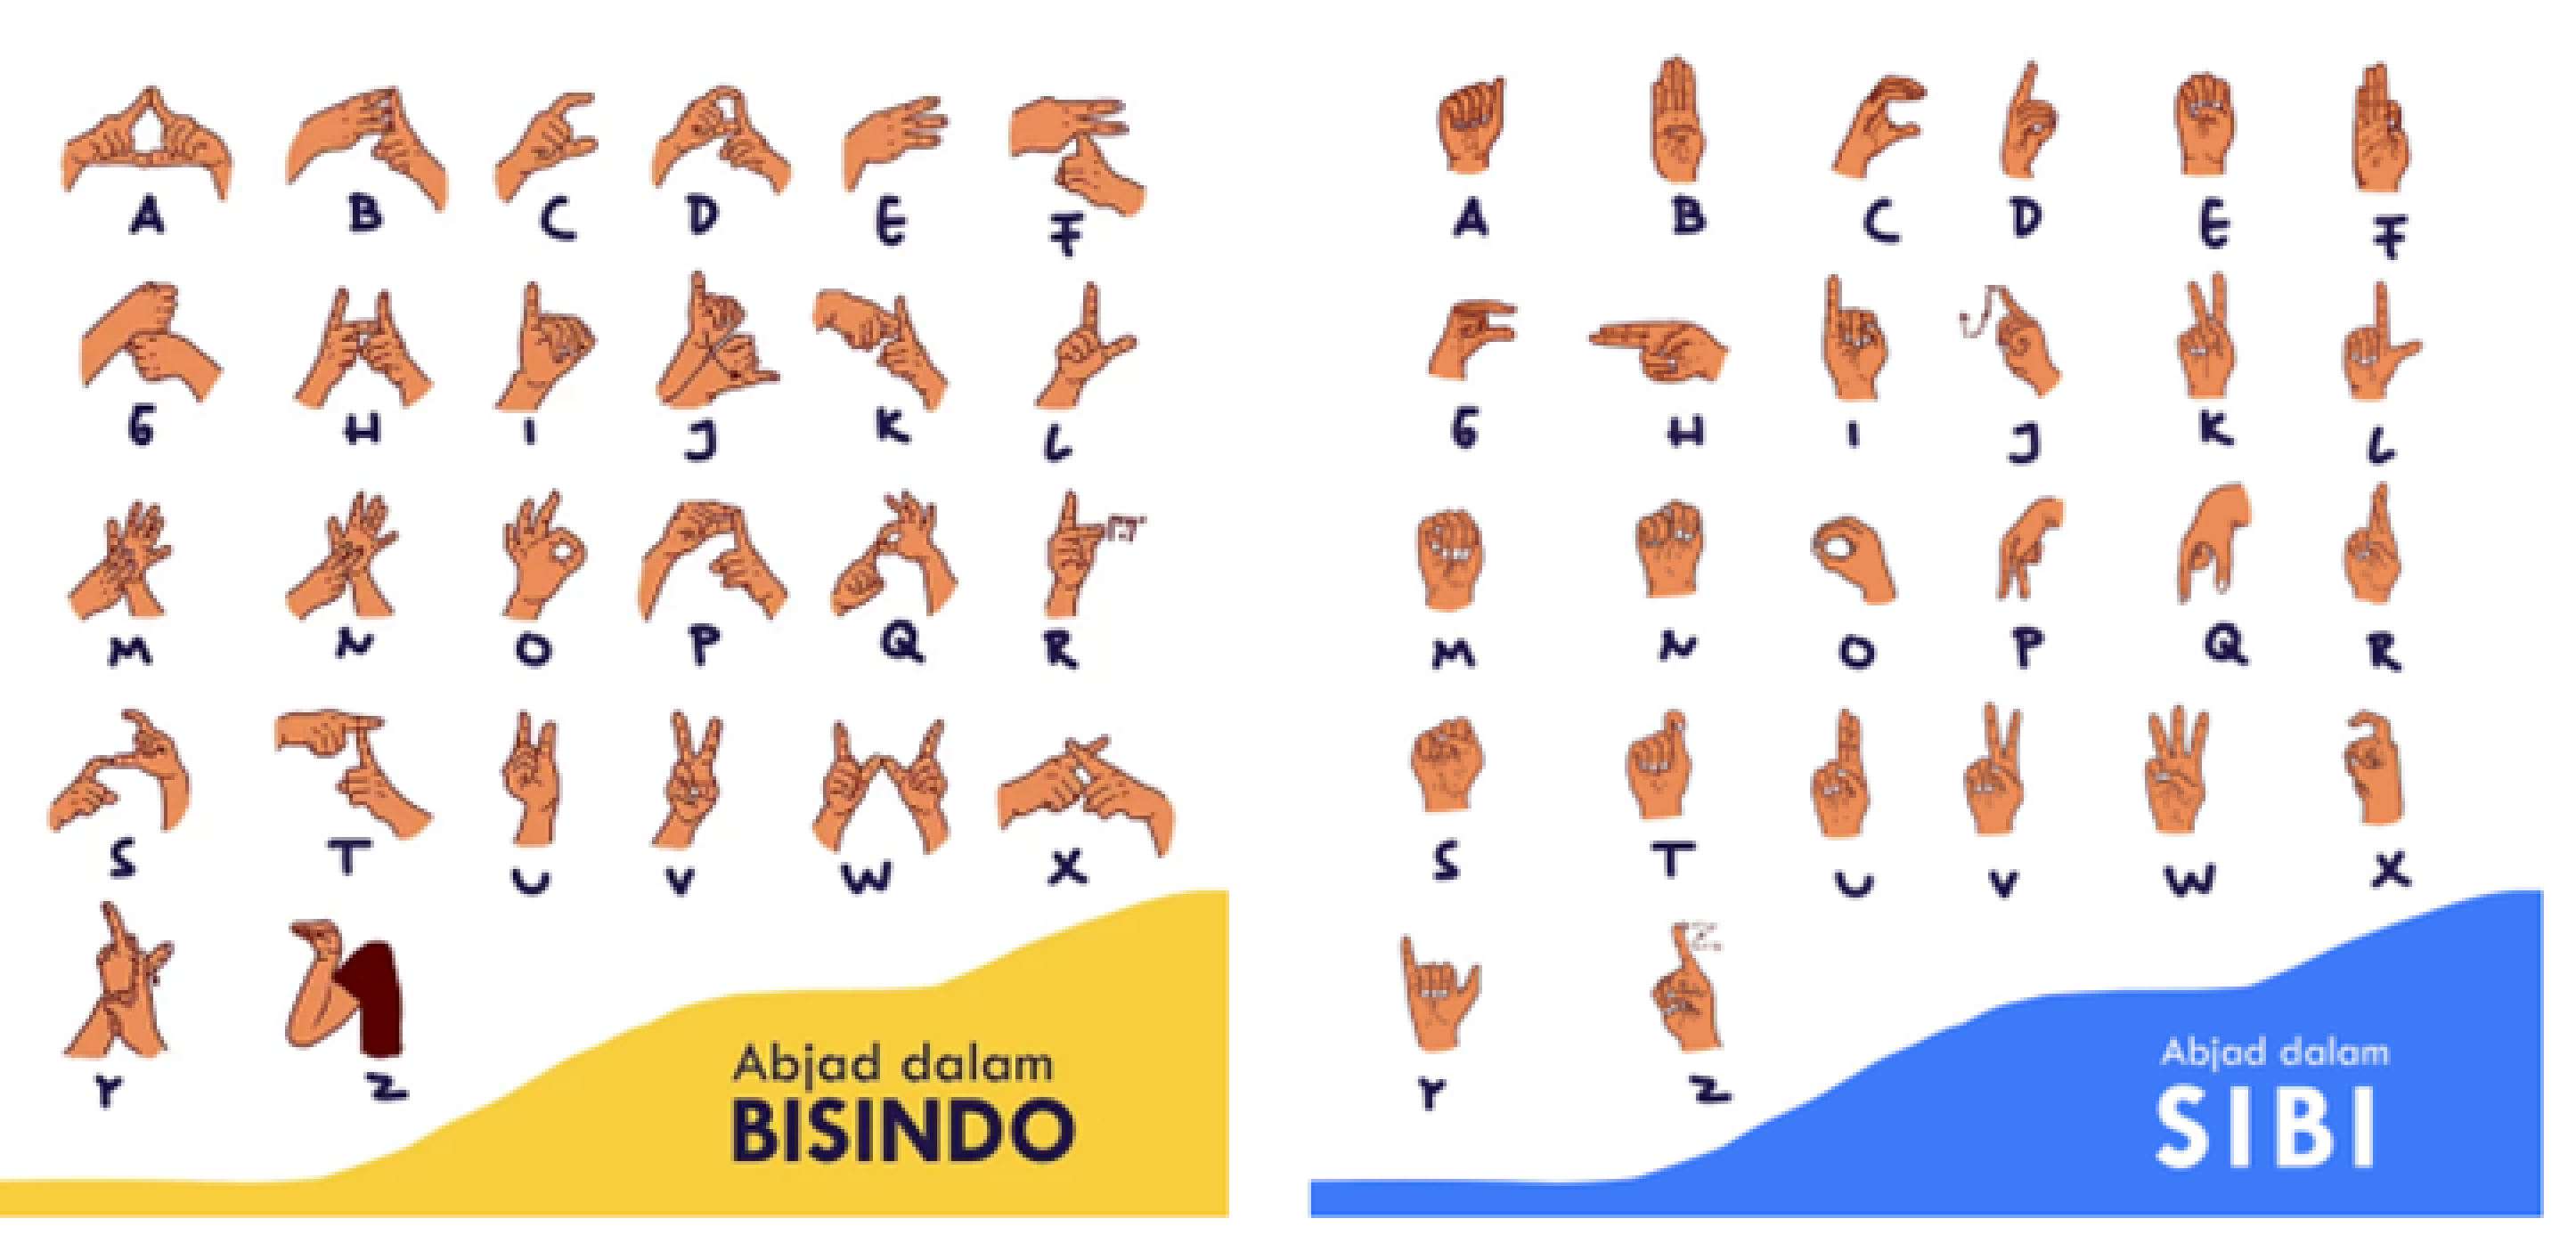
\includegraphics[scale=0.6]{gambar/bab2-isyarat-indonesia.png}
 
    \caption{Isyarat abjad dalam BISINDO dan SIBI}
    \label{fig:isyaratindonesia}
\end{figure}

Kekurangan pada indra pendengaran yang dialami oleh penyandang tunarungu menyebabkan perkembangan kemampuan berbahasa dan berbicara yang menurun, sehingga banyak dari penyandang tunarungu juga menderita tunawicara. Namun, hal ini bukan menjadi hambatan bagi penderta tunarungu dalam berkomunikasi dengan lingkungan sekitar. Bahasa isyarat adalah bahasa yang dilakukan dengan menggunakan gerakan - gerakan bada yang diiringi dengan ekspresi muka sebagai simbolisasi dari bahasa lisan yang ingin diungkapkan. Tunarungu menggunakan bahasa isyarat sebagai bahasa utama dalam berkomunikasi. Dalam mengungkapkan sesuatu, mereka menggunakan kombinasi antara bentuk tangan, orientasi dan gerak tangan, lengan tubuh, serta ekspresi wajah \parencite{mursita2015}.

Di Indonesia terdapat 2 bahasa isyarat yang berkembang, yaitu Sistem Bahasa Isyarat Indonesia (SIBI) dan Bahasa Isyarat Indonesia (BISINDO). Berdasarkan gambar \ref{fig:isyaratindonesia}, dapat dilihat bahwa SIBI membentuk isyarat dengan menggunakan 1 tangan saja, sedangkan BISINDO membentuk isyarat menggunakan 2 tangan. BISINDO merupakan isyarat alamiah yang diciptakan dan digunakan sendiri oleh penyandang tunarungu dengan pandangan dan persepsi mereka terhadap segala sesuatu di lingkungan sekitar mereka. Beragam objek atau konsep dapat dinyatakan melalui bahasa isyarat yang mencerminkan bentuk, karakteristik, atau visualnya. Namun, ketika suatu konsep terlalu abstrak untuk direpresentasikan, individu yang tunarungu biasanya akan mengkomunikasikannya dengan memanfaatkan abjad jari \parencite{wedayanti2019}. Tunarungu di Indonesia lebih memilih menggunakan BISINDO sebagai bahasa isyarat yang digunakan dalam kehidupan sehari – hari dibandingkan dengan SIBI karena kemudahan dalam pembentukan isyarat yang tidak terikat pada struktur baku bahasa Indonesia dengan disertai ekspresi wajah dalam pengungkapannya \parencite{handhika2018}. BISINDO sendiri berasal dari bahasa awal atau bahasa ibu tunarungu, dimana penggunaan BISINDO sendiri menyesuaikan dengan pemahaman bahasa tunarungu dari berbagai latar belakang tunarungu dengan tanpa menekankan pada struktur imbuhan bahasa Indonesia \parencite{mursita2015}

\subsection{MediaPipe}
MediaPipe merupakan suatu kerangka kerja (\emph{framework}) yang digunakan untuk membantun suatu pipline dalam melakukan inferensi pada data sensorik. MediaPipe memungkinkan untuk membangun suatu pipline yang terdiri dari komponen modular seperti inferensi model, algoritma pemrosesan media, dan transformasi data. Data sensorik seperti audio dan video dapat dimasukkan ke dalam grafik dan menghasilkan \emph{output} berupa deskripsi seperti penentuan objek dan penanda wajah. Kerangka ini mempermudah dalam pembuatan \emph{prototype} cepat dari pipeline persepsi dengan model inferensi dan komponen yang dapat digunakan Kembali. MediaPipe dapat mengabstraksikan dan menghubungkan model – model persepsi individu ke dalam alur yang dapat dipertahankan, dimana hal ini dapat memudahkan dalam penggunaan ulang komponen dalam berbagai aplikasi. Konsep dasar dari MediaPipe terdiri atas tiga bagian utama, yaitu kerangka kerja inferensi data sensorik, seperangkat alat evaluasi kinerja, dan kumpulan komponen inferensi dan pemrosesan yang dapat digunakan kembali. Pipa atau \emph{pipeline} dalam MediaPipe dapat diartikan sebagai grafik komponen yang diarahkan, dimana setiap komponen adalah suatu kalkulator yang spesifik. MediaPipe telah digunakan untuk berbagai aplikasi, termasuk deteksi objek, dan diancang untuk memudahkan dalam pengembangan model machine learning ataupun \emph{ deep learning}, seperti pada deteksi objek dan estimasi pose, terkhususnya pendeteksian gerakan bahasa isyarat \parencite{lugaresi2019:}.

\subsubsection{Mediapipe Pose}
Estimasi pose atau pose estimation merupakan suatu aspek yang memiliki peranan penting dalam berbagai teknologi saat ini, seperti mengukur latihan fisik, pengenalan bahasa isyarat, pendeteksian gerakan yoga, menari, dan kebugaran. MediaPipe pose terinspirasi oleh model BlazeFace yang digunakan dalam deteksi wajah Mediapipe, sebagai proksi untuk mendeteksi orang. Model ini dapat dikatakan terinspirasi oleh Virtuvian Leonardo, untuk memperkirakan titik Tengah pinggul seseorang, jari – jari lingkaran yang mengelilingin seluruh orang, dan sudut kemiringan garis yang menghubungkan titik tengah bahu dan pinggul. Model \emph{landmark} dari Mediapipe pose ini memprediksi total 33 lokasi \emph{landmark}, dengan diawali dari bagian hidung hingga diakhiri pada kaki bagian kanan \parencite{googleMediapipe}. 

\begin{figure}[H]
    \centering

    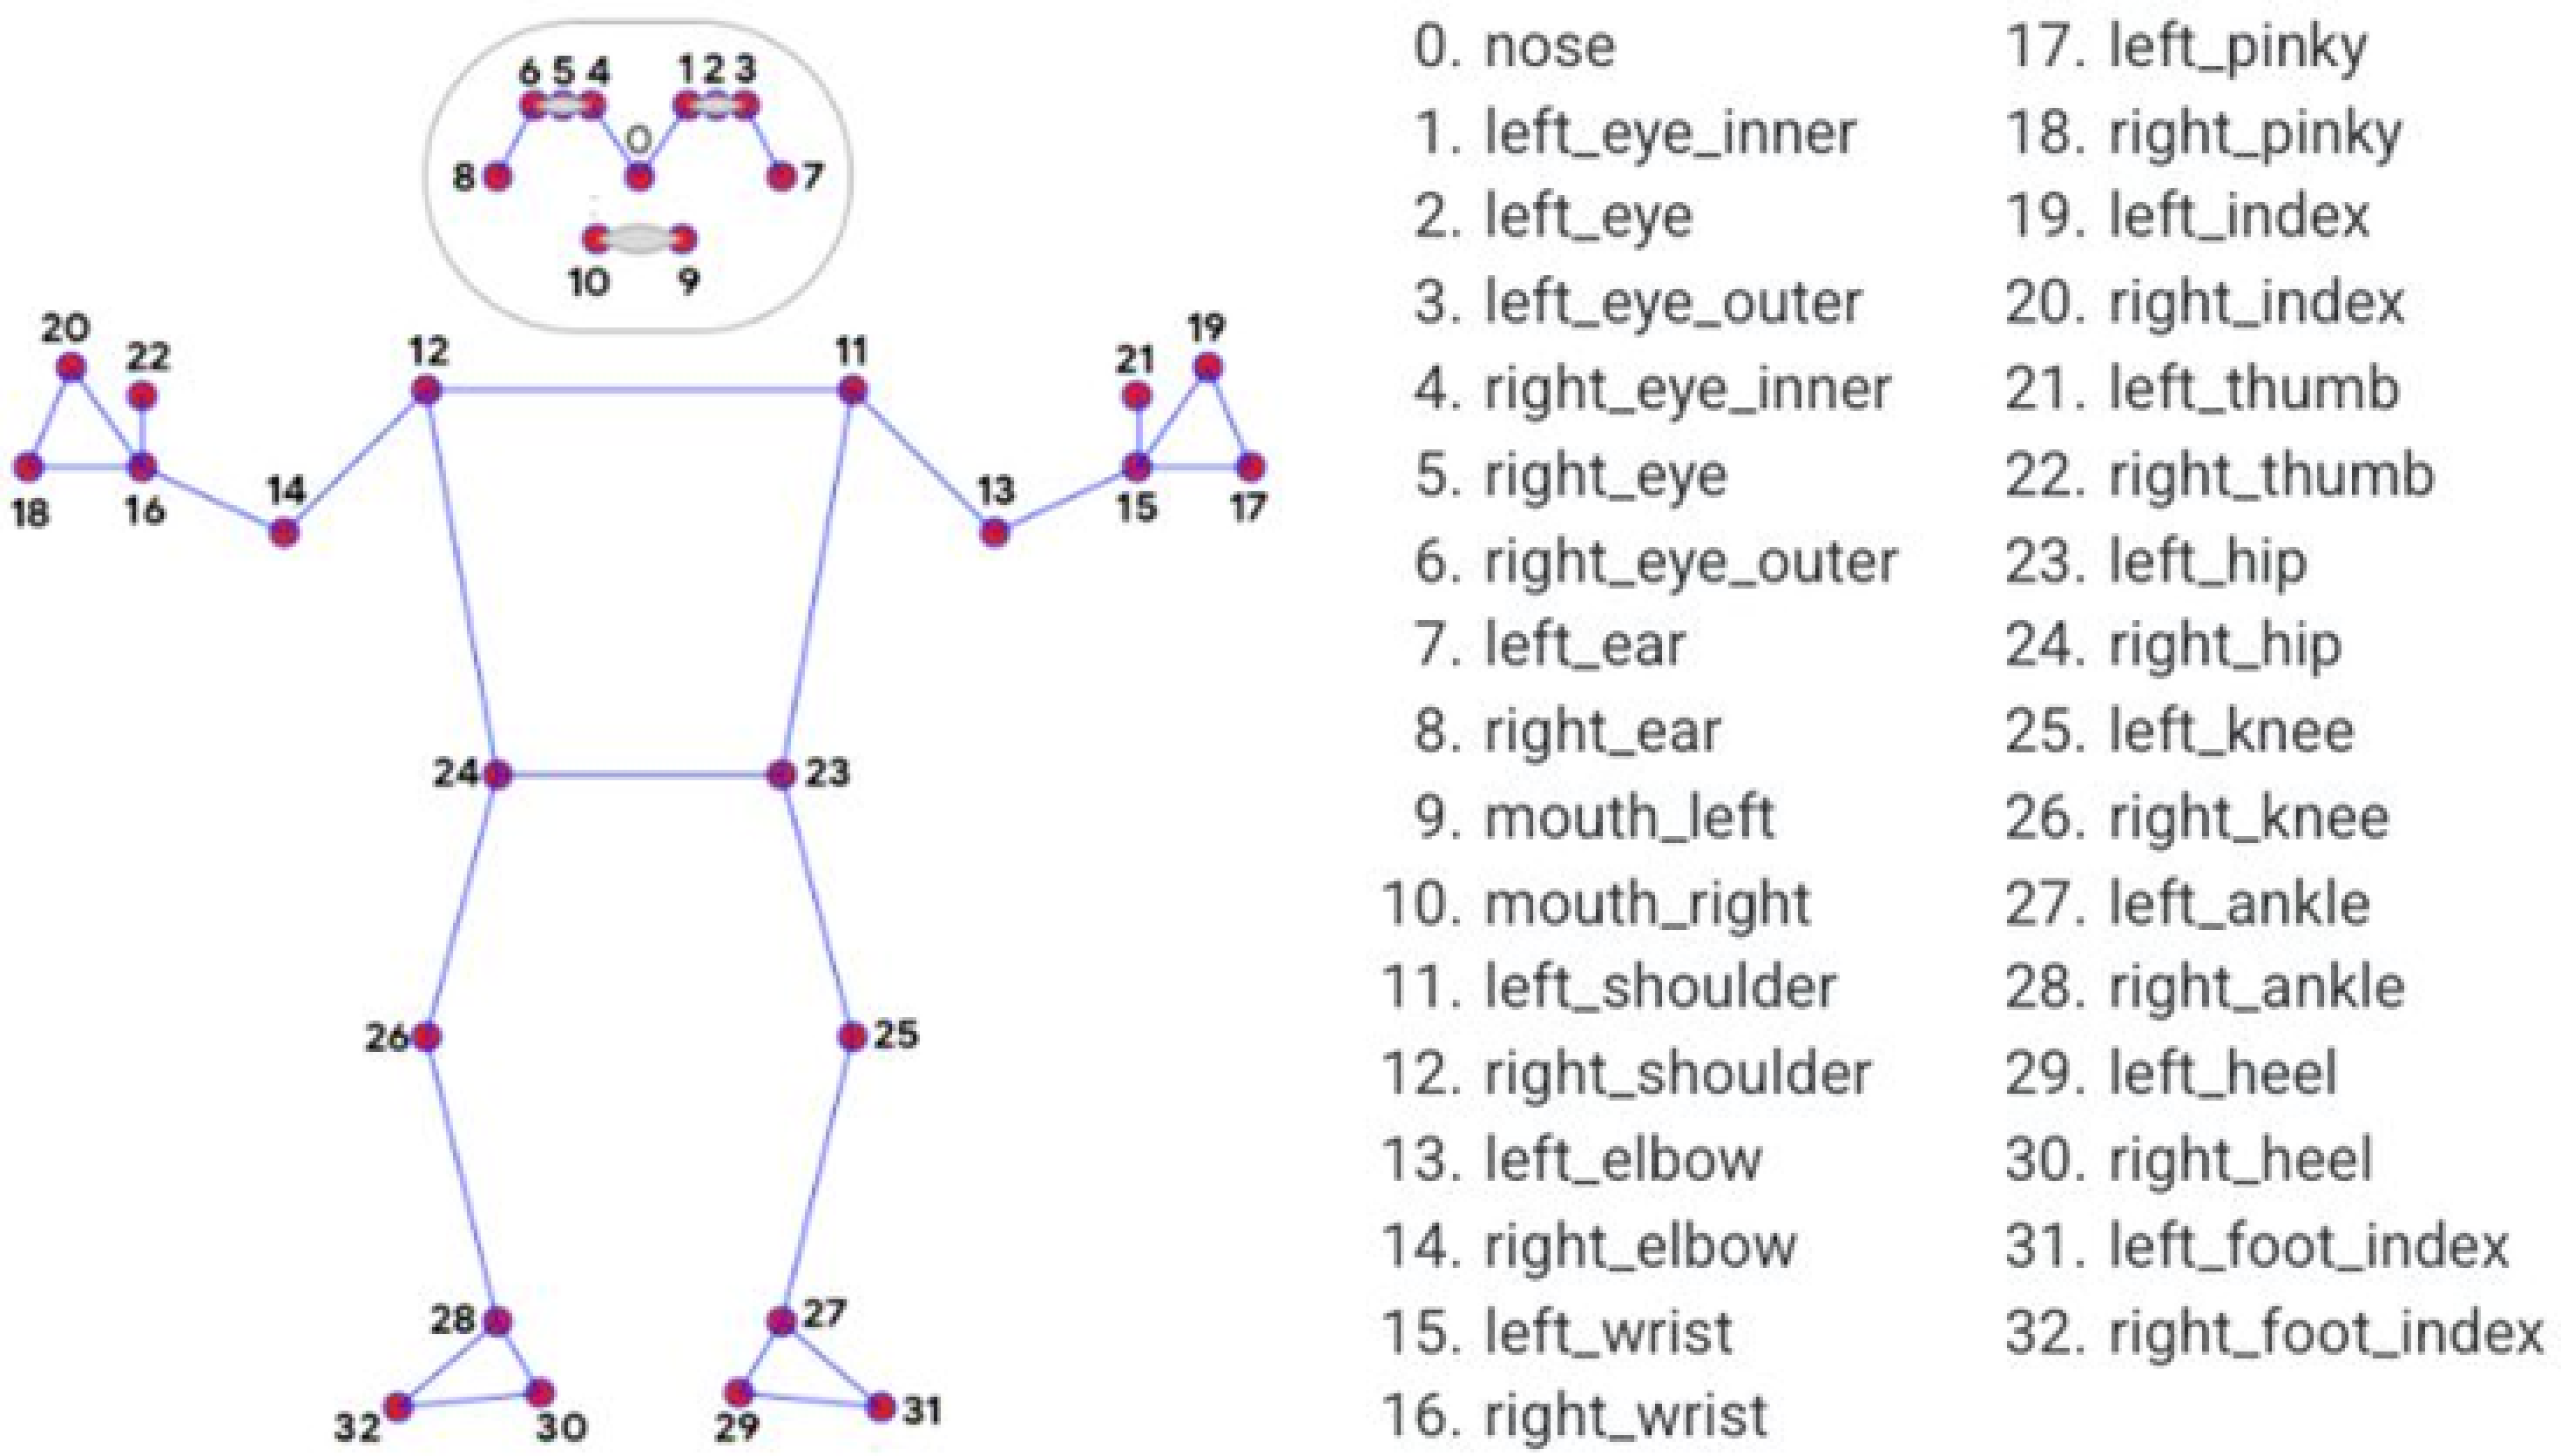
\includegraphics[scale=0.5]{gambar/bab2-mp-pose.png}
 
    \caption{\textit{Keypoints} \emph{landmark}s pada MediaPipe pose}
    \label{fig:mediapipepose}
\end{figure}

\subsubsection{Mediapipe Hand}
Kemampuan untuk merasakan bentuk dan gerakan tangan dapat menjadi komponen penting dalam meningkatkan pengalaman pengguna di berbagai platform teknologi, seperti pendeteksian gerakan tangan pada pembentukan bahasa isyarat yang memiliki artinya masing – masing. MediaPipe hand adalah solusi pelacakan tangan dan jari dengan ketelitian tinggi dengan menggunakan \textit{machine learning} untuk menyimpulkan 21 \emph{landmark} 3D tangan dari satu bingkai. Pada setiap ruas jari memiliki \emph{landmark}-nya tersendiri sehingga total \emph{landmark} dari 4 \emph{landmark} dan untuk pangkal telapak tangan terdapat 1 buah \emph{landmark} \parencite{googleMediapipe}.

\begin{figure}[H]
    \centering

    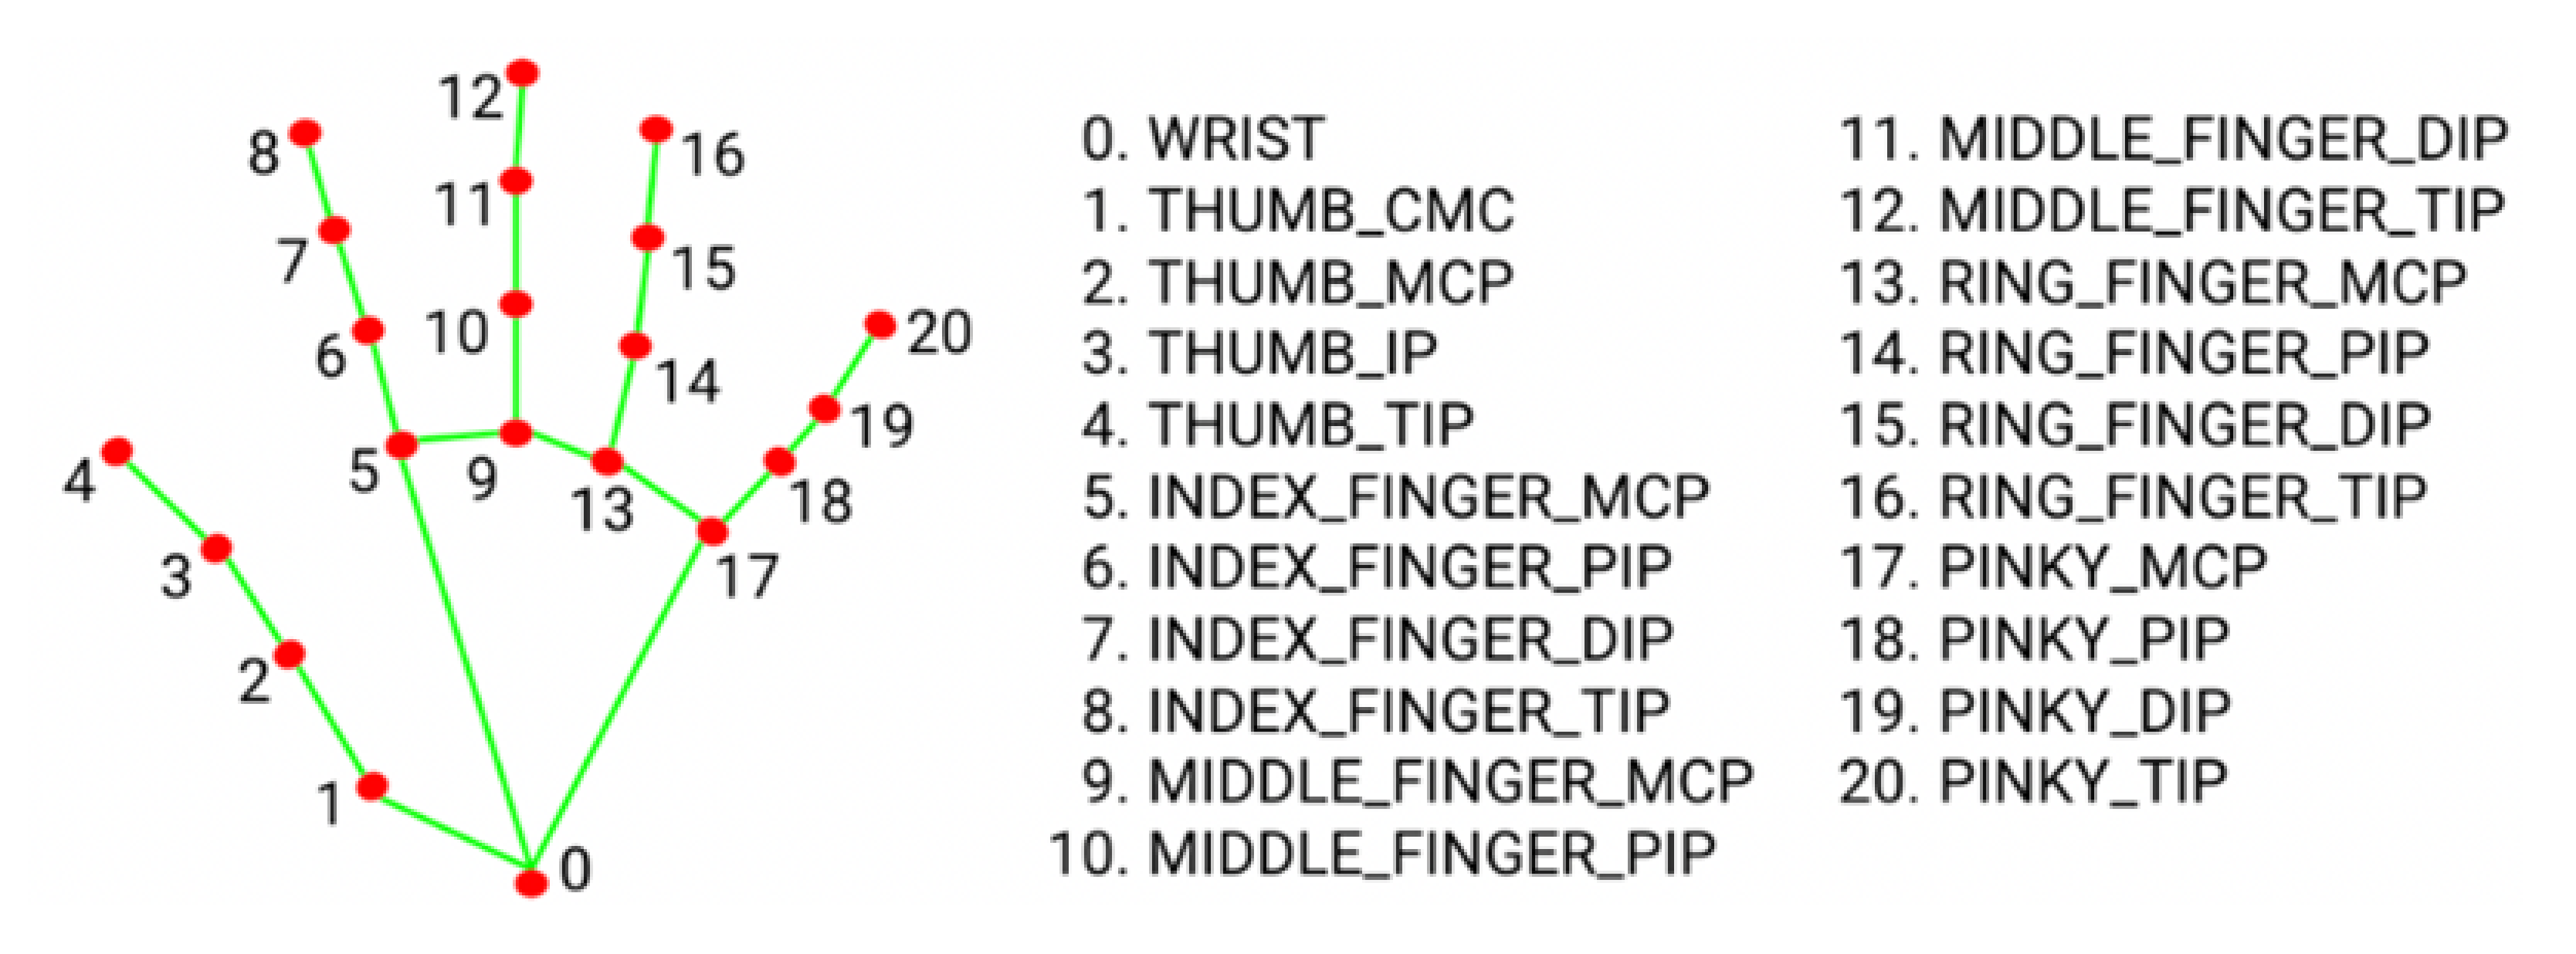
\includegraphics[scale=0.5]{gambar/bab2-mp-hand.png}
 
    \caption{\textit{Keypoints} \emph{landmark}s pada MediaPipe Hand}
    \label{fig:mediapipehand}
\end{figure}

\subsection{\textit{Long Short-Term Memory} (LSTM)}

\begin{figure}[H]
    \centering

    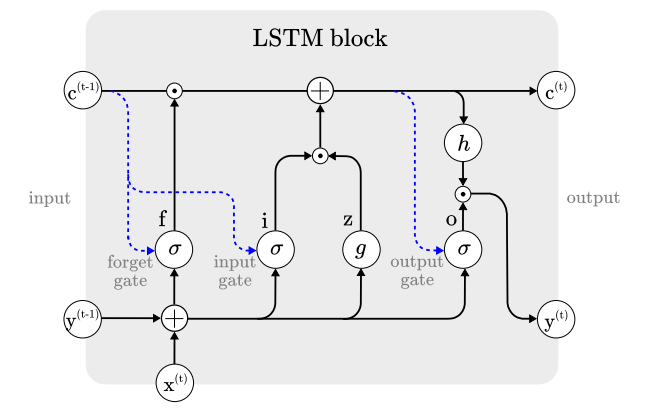
\includegraphics[scale=1.2]{gambar/bab2-lstm-model.png}
 
    \caption{Cara kerja arsitektur LSTM}
    \label{fig:longshortterm}
\end{figure}

\textit{Long Short-Term Memory} (LSTM) merupakan bentuk khusus dari neural network RNN atau \textit{Recurrent Neural Network} yang memiliki kemampuan \textit{feedback connection}. Kemampuan ini memungkinkan LSTM untuk dapat mengingat informasi untuk waktu yang lama sehingga dapat digunakan untuk menyelesaikan permasalahan yang memiliki sifat sekuensial atau berurutan. Keunggulan LSTM jika dibandingkan dengan RNN adalah LSTM memiliki kemampuan untuk mengingat informasi yang lebih baik dan efektif sehingga meminimalisir terjadinya kehilangan informasi yang umum terjadi pada pemrosesan informasi lama yang panjang pada penggunaan RNN \parencite{xia2020}. Oleh karena itu, LSTM cocok untuk dimanfaatkan dalam pengembangan suatu sistem penerjemah isyarat yang mana membutuhkan kemampuan dalam mengingat gerakan bahasa isyarat yang bersifat sekuensial untuk kemudian disimpan dan diterjemahkan ketika terdapat gerakan yang sesuai.

Pada gambar \ref{fig:modelLSTM}, \textit{Long Short-Term Memory} tersusun atas beberapa layer yang meliputi \textit{block input}, \textit{input gate}, \textit{forget gate}, \textit{cell}, \textit{output gate}, dan \textit{block output}. \textit{Block input} bertindak untuk melakukan pembaharuan terhadap $x^{(t)}$ dengan \textit{Block input} LSTM unit $y^{(t-1)}$ pada iterasi terakhir. Hal ini dapat dirumuskan sebagai berikut:

\begin{equation}
  \label{eq:blockinputLSTM}
  x^{(t)} = g(W_z x^{(t)} + R_z y^{(t-1)} + b_z)
\end{equation}

Pada rumus \ref{eq:blockinputLSTM}, $W_z$ dan $R_z$ merupakan \textit{weight} yang diasosiasikan dengan $x^{(t-1)}$ dan $y^{(t-1)}$ secara berurutan. Sedangkan $b_z$ diartikan sebagai \textit{weight bias vector}. Paada \textit{layer} ini, LSTM   Pada input gate, akan dilakukan pembaharuan terhadap \textit{input} saat ini, ($x^{(t)}$), \textit{output} dari unit LSTM ($y^{(t-1)}$), dan nilai dari \textit{cell} ($c^{(t-1)}$) pada iterasi terakhir. Hal ini  dapat dirumuskan sebagai:

\begin{equation}
    \label{eq:inputgateLSTM}
    i^{(t)} = \sigma(W_i x^{(t)} + R_i y^{(t-1)}+ p_i \odot c^{(t-1)} + b_i)
\end{equation}

Pada rumus \ref{eq:inputgateLSTM}, $\odot$ melambangkan perkalian titik antara 2 buah vector. $W_i$, $WR_i$, dan $p_i$ adalah weight yang dimiliki oleh $x^{(t)}$, $y^{(t-1)}$, dan $c^{(t-1)}$. Sementara $b_i$ merepresentasikan bias vector yang diasosasikan oleh unit ini. Forget gate bertindak untuk menentukan informasi yang harus dihapus dari \textit{cell state} ($c^{(t-1)}$) sebelumnya. Oleh karena itu, nilai fungsi aktivasi dari \textit{forget gates} pada \textit{time step} t dihitung berdasarkan input saat ini ($x^{(t)}$), \textit{ouput} ($y^{(t - 1)}$), \textit{state memory cell} ($y^{(t - 1)}$) pada \textit{time step} sebelumnya ($t - 1$), koneksi \textit{peephole}, dan \textit{bias} dari \textit{forget gate} itu sendiri (${b_f}$). \textit{Forget gate} dapat dirumuskan sebagai:

\begin{equation}
    \label{eq:forgetgateLSTM}
    f^{(t)} = \sigma(W_f x^{(t)} + R_f y^{(t-1)}+ p_f \odot c^{(t-1)} + b_f)
\end{equation}

Pada rumus \ref{eq:forgetgateLSTM}, $W_f$, $R_f$, dan $p_f$ adalah \textit{weight} yang diasosiasikan dengan $x^{(t)}$, $y^{(t-1)}$, dan $c^{(t-1)}$. Sementara $b_i$ merepresentasikan bias vector yang diasosasikan oleh unit ini. \textit{Cell} merupakan bagian yang melakukan komputasi untuk nilai dari \textit{cell} itu sendiri yang merupakan gabungan dari nilai - nilai pada input $z^{(t)}$, input gate $i^{(t)}$, dan \textit{forget gate} $f^{(t)}$ dengan nilai pada \textit{cell} sebelumnya. Hal ini dapat dirumuskan sebagai:

\begin{equation}
    \label{eq:cellLSTM}
    c^{(t)} =  z^{(t)} \odot  i^{(t)} + z^{(t-1)} \odot  f^{(t)}
\end{equation}

Pada \textit{output gate}, akan dilakukan perhitungan untuk \textit{input} saat ini $x^{(t)}$, \textit{output} dari LSTM unit $y^{(t-1)}$, dan nilai cell $c^{(t-1)}$ pada iterasi terakhir. Hal ini dapat dirumuskan sebagai:

\begin{equation}
    \label{eq:outputgateLSTM}
    o^{(t)} = \sigma(W_o x^{(t)} + R_o y^{(t-1)}+ p_o \odot c^{(t)} + b_o)
\end{equation}

Pada rumus \ref{eq:outputgateLSTM}, $W_f$, $R_f$, dan $p_f$ adalah\textit{weight} yang diasosiasikan dengan $x^{(t)}$, $y^{(t-1)}$, dan $c^{(t-1)}$. Sementara $b_i$ merepresentasikan \textit{bias vector} yang diasosasikan oleh unit ini. Pada \textit{block otuput}, akan dihitung nilai \textit{cell} saat ini $(c^{(t)})$ dengan nilai output gate saat ini. Hal ini dapat dirumuskan sebagai berikut:

\begin{equation}
    \label{eq:blockoutputLSTM}
    c^{(t)} =  g(c^{(t)}) \odot o^{(t)}
\end{equation}

Pada persamaan - persamaan diatas, $\sigma$, $g$, $h$ melambangkan fungsi aktivasi non-linear antar titik. Fungsi logistik \textit{sigmoid} $(\sigma(x) = \frac{1}{1 + e^{-x}})$ digunakan sebagai fungsi aktivasi pada \textit{gate}. Sedangkan fungsi aktivasi \textit{hyperbolic} tangent $g(x) = h(x) = tanh(x)$ digunakan seabagai aktivasi fungsi pada \textit{block input} dan \textit{output} \parencite{van2020}.

\subsection{Intel \emph{Next Unit Computing} (NUC)}

\begin{figure}[H]
    \centering

    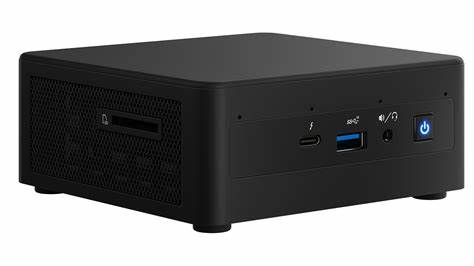
\includegraphics[scale=0.6]{gambar/bab2-nuc_11_performace_kit.jpeg}
 
    \caption{Intel NUC 11 \emph{Performance Kit}}
    \label{fig:jetsonnano}
\end{figure}

Intel \emph{Next Unit Computing} (NUC) merupakan komputer \emph{barebone} dengan ukuran kecil yang dirancang oleh Intel. Intel NUC merupakan perangkat yang berfokus dalam menyediakan komputasi kuat dalam ukuran yang praktis dan dapat melayani berbagai kebutuhan pengguna, mulai dari bermain \emph{game}, bisnis, hingga menjalankan aplikasi kompleks. Intel NUC secara resmi memperkenalkan perangkat ini pada tahun 2012 dan dipasarkan secara umum pada awal tahun 2013 \parencite{IntelNUC2020}. Adapun seri pertama dari Intel NUC memiliki CPU Sandy Bridger berbasis Celeron. Intel NUC telah berkembang hingga generasi ke-12 bernama Dragon Canyon yang dilengkapi dengan CPU Intel generasi ke-12 dan PCI Express Gen 5 \parencite{Halfacree2013}.

Intel NUC 11 merupakan perangkat Intel yang dirilis pada 13 Januari 2021 dengan kode nama Phantom Canyon. Salah satu model yang cukup banyak digunakan adalah Intel NUC 11 Performance Kit model NUC11PAHi7. Inti dari perangkat ini dilengkapi dengan prossesor Intel Core i7-1165G7. Prossesor ini memiliki quad-core yang memiliki kecepatan dasar 2.8 GHz dan dapat meningkat hingga 4.7 GHz.  Prossesor ini didukung oleh kartu grafis Iris XE yang menawarkan peningkatan kinerja grafis yang substansial dibandingkan dengan generasi sebelumnya. Hal ini memudahkan perangkat dalam menjalankan tugas mulai dari pengeditan video hingga bermain \emph{game}. Dari segi memori, Intel NUC 11 Performance Kit model NUC11PAHi7 mendukung hingga 64GB DDR4-3200 SODIMM dual-channel, menyediakan ruang yang luas untuk multitasking intensif. Untuk penyimpanan, perangkat ini menawarkan slot M.2 yang fleksibel yang mendukung SSD NVMe terbaru dengan memastikan kecepatan akses dan penyimpanan data yang cepat. Hal ini kritikal untuk aplikasi yang melibatkan set data besar atau pemrosesan \emph{realtime}. Konektivitas adalah salah satu kekuatan utama model ini, menampilkan berbagai pilihan termasuk Thunderbolt 4, HDMI 2.0b, dan beberapa port USB 3.1. Ini memungkinkan koneksi banyak periferal dan tampilan secara bersamaan, meningkatkan produktivitas dan fleksibilitas dalam skenario penggunaan. Selain itu, dengan Intel Wi-Fi 6 dan Bluetooth 5.1, Intel NUC 11 pada model ini menawarkan konektivitas nirkabel terdepan untuk integrasi yang mulus ke dalam lingkungan jaringan apa pun. Dimensi yang ringkas untuk model ini NUC11PAHi70Z, yang hanya berukuran 117 x 112 x 51 mm dapat menjadikannya pilihan ideal untuk lingkungan di mana ruang terbatas \parencite{ASUS2024}. Kombinasi komputasi berkinerja tinggi, kemampuan grafis yang kuat, dan opsi konektivitas yang luas, semua dalam bentuk yang kecil, menonjolkan NUC11PAHi70Z sebagai pilihan teratas bagi pengguna yang membutuhkan solusi komputasi yang kuat, serbaguna, dan efisien ruang.

% \subsection{Jetson Nano}
% \begin{figure}[H]
%     \centering

%     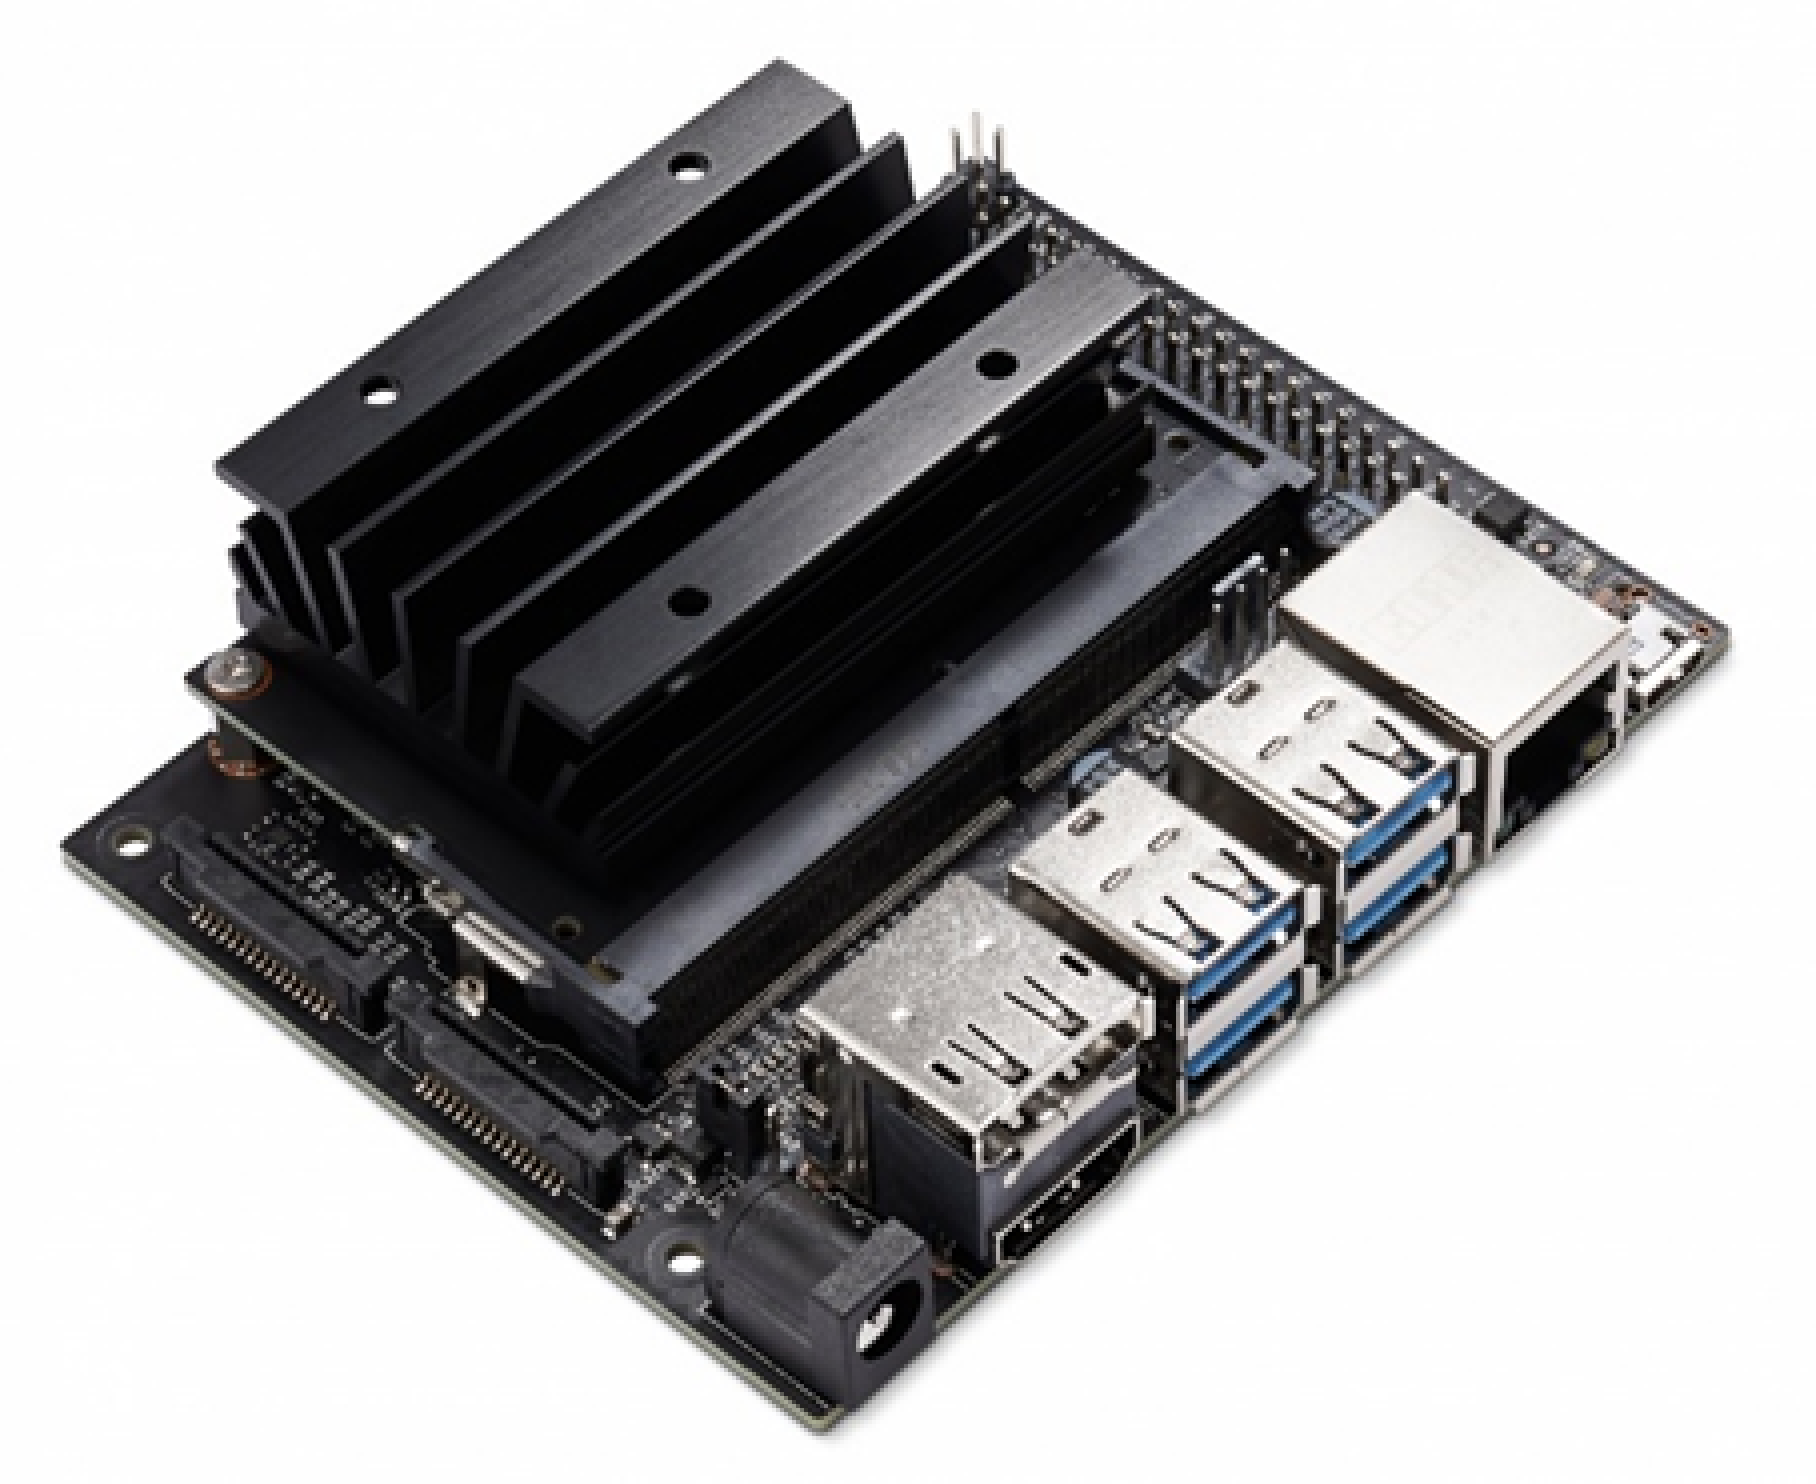
\includegraphics[scale=0.6]{gambar/bab2-jetson-nano.png}
 
%     \caption{Jetson Nano Developer Kit}
%     \label{fig:jetsonnano}
% \end{figure}

% Jetson Nano adalah perangkat komputasi keluaran NVIDIA yang didedikasikan dalam pengembangan \textit{machine lerarning} dan komputasi edge. Jetson Nano memiliki kemampuan untuk dapat menjalankan beberapa neural networks secara paralel. Kemampuan ini memungkinkan Jetson Nano untuk digunakan dalam \textit{image clasiification}, \textit{object detection}, \textit{segmentation}, dan \textit{speech processing} \parencite{nvidiaJetsonNano}. Perangkat ini dapat menjadi solusi dalam menjalankan model \textit{machine learning} atau \textit{deep learning} pada perangkat portable dan hemat energi. 

% Perangkat ini dilengkapi dengan 128 NVIDIA CUDA cores. Ditenagai oleh prosesor Quad-core ARM Cortex-A57 MPCore, platform ini menyediakan fungsionalitas komputasi yang solid dengan memori 4 GB 64-bit LPDDR4 yang beroperasi pada 1600MHz, memberikan bandwidth 25.6 GB/s. Untuk penyimpanan, Jetson Nano dilengkapi dengan 16 GB eMMC 5.1, yang memberikan ruang yang cukup untuk aplikasi dan data pengguna. Dalam konteks pengkodean video, perangkat ini dapat mengkodekan video dengan kecepatan 250MP/sec, mendukung format seperti 1x 4K pada 30fps (HEVC), 2x 1080p pada 60fps (HEVC), dan sebagainya. Sementara itu, untuk decode video, perangkat ini menawarkan kemampuan hingga 500MP/sec, dengan dukungan untuk format seperti 1x 4K pada 60fps (HEVC) dan 2x 4K pada 30fps (HEVC). Jetson Nano juga dilengkapi dengan 12 jalur kamera (3x4 atau 4x2) MIPI CSI-2 D-PHY 1.1, yang mendukung kecepatan hingga 1.5 Gb/s per pasangan, memberikan fleksibilitas dalam pengembangan aplikasi berbasis kamera. Dalam hal konektivitas, perangkat ini menawarkan Gigabit Ethernet dan M.2 Key E, serta kemampuan tampilan melalui HDMI 2.0 dan eDP 1.4. Jetson Nano juga dilengkapi dengan 4x USB 3.0 dan USB 2.0 Micro-B, serta berbagai opsi konektivitas lainnya seperti GPIO, I2C, I2S, SPI, dan UART, semuanya dalam form factor mekanis 69.6 mm x 45 mm dengan konektor tepi 260-pin \parencite{nvidiaJetsonNano}.

\subsection{Performa Klasifikasi}

\begin{figure}[H]
    \centering

    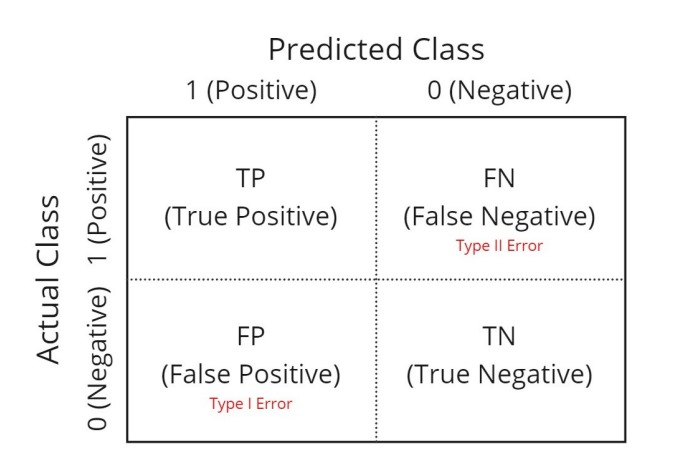
\includegraphics[scale=0.8]{gambar/bab2-confusion-matrix.png}
 
    \caption{\textit{Confusion matrix}}
    \label{fig:confusionMatrix}
\end{figure}

Dalam melakukan klasifikasi dengan model, diperlukan adanya suatu tolak ukur berdasarkan serangkaian dataset pengujian yang diberikan. Salah satu metode yang dapat digunakan adalah dengan menggunakan \textit{confusion matrix}. \textit{Confusion matrix} merupakan sebuah konsep yang umum digunakan dalam menentukan performa klasifikasi model dengan memberikan informasi mengenai data aktual dan data prediksi model klasifikasi. Berdasarkan \ref{fig:confusionMatrix} \textit{confusion matrix} memiliki bentuk matrix 2 dimensi, dimana satu dimensi memiliki index yang berisikan data aktual dari \textit{class} obyek klasifikasi dan satu dimensi lainnya memiliki index yang berisikan data klasifikasi yang dihasilkan oleh model \parencite{deng2016}. 

Pada \textit{confusion matrix}, terdapat empat aspek yang digunakan untuk merepresentasikan perbandingan dari kelas aktual dan kelas prediksi. Keempat aspek tersebut meliputi \textit{true positive}, \textit{true negative}, \textit{false positive}, \textit{true negative}. \textit{True positive} (TP) merupakan kondisi dimana data aktual bernilai 1 (positif) diprediksi sebagai data yang bernilai 1 (positif). Sedangkan \textit{true negative} (TN) merupakan kondisi dimana data aktual bernilai 0 (negatif) diprediksi sebagai data yang bernilai 0 (negatif). \textit{False positive} (FP) merupakan kondisi dimana data aktual bernilai 0 (negatif) diprediksi sebagai data yang bernilai 1 (positif). Sedangkan \textit{false negative} (TN) merupakan kondisi dimana data aktual bernilai 1 (positif) diprediksi sebagai data yang bernilai 0 (negatif) \parencite{shajihan2020}. Keempat aspek ini kemudian dapat dihitung nilai \textit{accuracy}, \textit{precision}, \textit{recall}, \textit{F-score} yang dapat membantu dalam memahami performa klasifikasi model dengan lebih detail lagi.

\subsubsection{\textit{Accuracy}}
\textit{Accuracy} merupakan metode untuk mengevaluasi kinerja yang menunjukkan tingkat ketep\\atan sebuah model dalam mengklasifikasikan data pengujian yang diberikan secara akurat. \textit{Accuracy} dapat diartikan sebagai perbandingan antara prediksi benar (TP dan TN) terhadap keseluruhan data yang ada. Secara sederhana, \textit{accuracy} menggambarkan seberapa dekat nilai prediksi berada dengan nilai sebenarnya. \textit{Accuracy} dapat dirumuskan dirumuskan pada persamaan \ref{eq:perofrmaAccuracy} \parencite{OvalleMagallanes2020}
   
\begin{equation}
    \label{eq:perofrmaAccuracy}
    Accuracy = \frac{TP + TN}{TP + TN + FP + FN}
\end{equation}

\subsubsection{\textit{Precision}}
\textit{Precision} merupakan metode untuk mengevaluasi kinerja yang mengukur seberapa akurat data yang diminta cocok dengan hasil prediksi yang diberikan oleh model. \textit{Precision} dapat diartikan sebagai perbandingan antara prediksi benar positif (TP) terhadap total hasil yang diprediksi positif (jumlah TP dan FP). \textit{Precision} dapat irumuskan pada persamaan \ref{eq:perofrmaPrecision} \parencite{OvalleMagallanes2020}

\begin{equation}
    \label{eq:perofrmaPrecision}
    Precision = \frac{TP}{TP + FP}
\end{equation}

\subsubsection{\textit{Recall}}
\textit{Recall} merupakan metode untuk menunjukkan kemmapuan sebuah model untuk secara akurat mengidentifikasi informasi yang relevan. Recall dapat diartikan sebagai perbandingan antara umlah prediksi benar positif (TP) dengan total jumlah data aktual positif (jumlah TP dan FN). textit{Recall dapat dirumuskan pada persamaan \ref{eq:perofrmaRecall} \parencite{OvalleMagallanes2020}

\begin{equation}
    \label{eq:perofrmaRecall}
    Recall = \frac{TP}{TP + FN}
\end{equation}

\subsubsection{\textit{F-Score}}

\textit{F-Score} adalah nilai yang berkisar antara nol hingga satu yang diperoleh dari rata - rata tertimbang (\textit{harmonic mean}) antara nilai precision dan recall. \textit{F-Score} dapat dirumuskan pada persamaan \parencite{Deng2016}

\begin{equation}
    \label{eq:perofrmaFScore}
    F{-}Score = \frac{2 \times {Precision} \times {Recall}}{{Precision} + {Recall}}
\end{equation}

% \label{subsec:hukumnewton}

% Newton \parencite{newton1687} pernah merumuskan bahwa \lipsum[1]
% Kemudian menjadi persamaan seperti pada persamaan \ref{eq:hukumpertamanewton}.

% Contoh pembuatan persamaan
% \begin{equation}
%   \label{eq:hukumpertamanewton}
%   \sum \mathbf{F} = 0\; \Leftrightarrow\; \frac{\mathrm{d} \mathbf{v} }{\mathrm{d}t} = 0.
% \end{equation}

% \subsection{Anti Gravitasi}
% \label{subsec:antigravitasi}

% Anti gravitasi merupakan \lipsum[1]


% % Contoh input gambar
% \begin{figure}[H]
%   \centering

%   % Ubah dengan nama file gambar dan ukuran yang akan digunakan
%   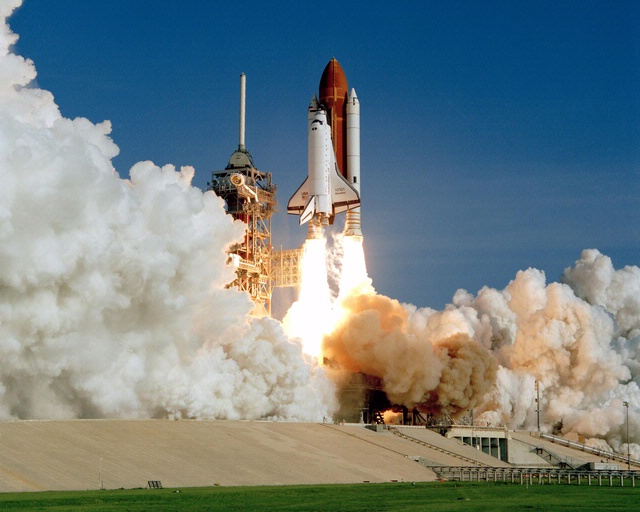
\includegraphics[scale=0.35]{gambar/roketluarangkasa.jpg}

%   % Ubah dengan keterangan gambar yang diinginkan
%   \caption{Peluncuran roket luar angkasa \emph{Discovery} \parencite{roketluarangkasa}.}
%   \label{fig:roketluarangkasa}
% \end{figure}

% Roket luar angkasa merupakan \lipsum[1]

% \emph{Discovery}, Gambar \ref{fig:roketluarangkasa}, merupakan \lipsum[2]
\cleardoublepage

% Bab 3 desain dan implementasi
\chapter{METODOLOGI}
\label{chap:metodologi}

% Ubah bagian-bagian berikut dengan isi dari desain dan implementasi

% Penelitian ini dilaksanakan sesuai \lipsum[1][1-5]
% \section{Data dan Peralatan}
% Adapun tata pendukung berupa data dan peralatan yang digunakan dalam pelaksanaan penelitian tugas akhir ini adalah sebagai berikut:

% \noindent \textbf{Data}\\
% Data yang akan digunakan merupakan kumpulan citra berukuran 640px x 480px. Kumpulan citra ini didapat melalui ekstraksi video yang berisi pengucapan bahasa isyarat BISINDO. Kumpulan citra ini dibuat secara mandiri oleh penulis menyesuaikan dengan kebutuhan kosakata isyarat dan kosakata tambahan yang dibutuhkan.

% \noindent \textbf{Peralatan}\\
% Adapun peralatan yang digunakan dalam penelitian tugas akhir ini adalah sebagai berikut:

% \begin{itemize}
%   \item Visual Studio Code
%   \item Anaconda
%   % \item Jetson Nano B01 Developer Kit
%   \item Intel Next Unit Computing (NUC) 
%   \item Webcam
%   \item Speaker
%   \item Laptop
% \end{itemize}

Tugas akhir ini akan dilaksanakan sesuai dengan desain sistem beserta implementasinya yang akan dibahas pada bab ini. Desain sistem ini merupakan konsep dasar perancangan dan pembuatan program pada tugas akhir ini. Desain sistem ini direpresentasikan dalam bentuk blok diagram yang diselesaikan secara bertahap dan menyeluruh.

\section{Metode yang Digunakan}

% Penelitian tugas akhir ini dilaksankaan sesuai dengan desain sistem yang tertera pada bab ini. Desain sistem yang dibuat merupakan konsep dari perancangan dan implementasi penelitian ini. Blok diagram pada gambar \ref{fig:blockdiagrammethod} merupakan serangkaian alur yang diikuti dalam pelaksanaan dan pengimplementasian tugas akhir ini.

Adapun tugas akhir ini merupakan pengembangan dari teknologi visi komputer yang kemudian diimplementasikan pada Intel \emph{Next Unit Computing} (NUC). Secara umum, pelaksanaan tugas akhir ini didasari oleh blok diagram yang dapat dilihat pada gambar \ref{fig:blockdiagrammethod}.

\begin{figure}[H]
  \centering

  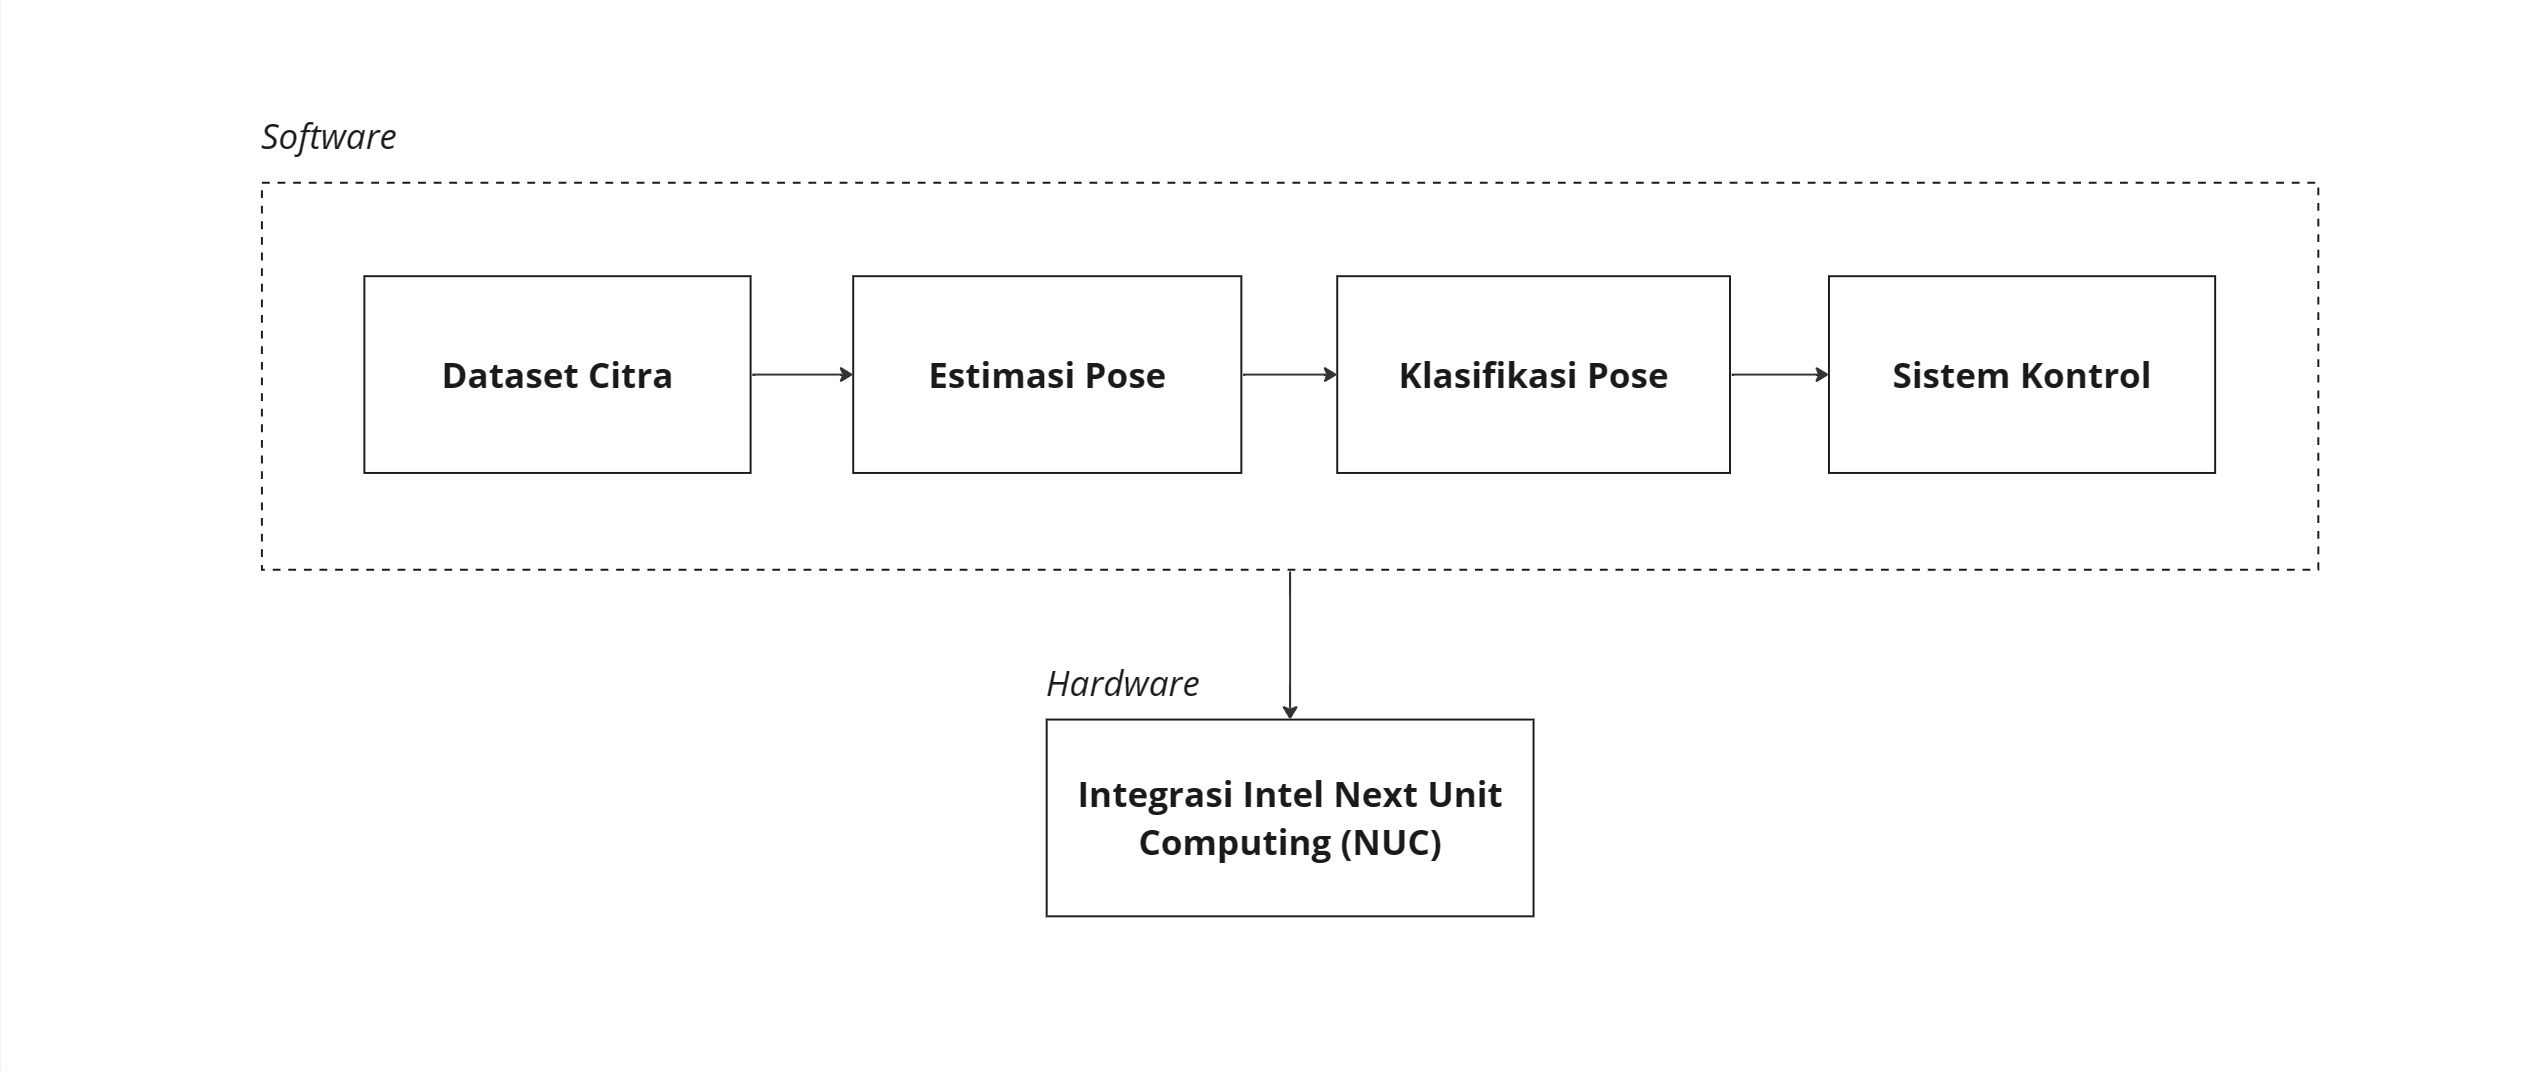
\includegraphics[scale=0.16]{gambar/bab3-block-diagram-nuc.jpg}

  \caption{Blok diagram metodologi}
  \label{fig:blockdiagrammethod}
\end{figure}

\subsection{Dataset Citra}
\label{sec:metodologidataset}

% Dataset yang akan digunakan pada tugas akhir ini merupakan kumpulan citra yang berbentuk sekuensial atau berurutan. Pengambilan dataset dilakukan di dalam ruangan tertutup dengan jarak bervariasi antara 1 - 2 meter dari kamera laptop dengan posisi setengah berdiri (dari pinggang hinga kepala). Data video yang didapatkan kemudian diproses melalui \textit{library} Python OpenCV sehingga dihasilkan citra. Pengambilan citra dilakukan sebesar 30 \textit{frame per second} (FPS) sehingga dalam satu detik terdapat 30 citra. Pembatasan FPS ini diharapkan dapat memberikan hasil yang stabil dan konsisten dalam pengambilan citra. Citra akan disimpan pada laptop secara lokal sehingga dapat diamati nantinya apakah gerakan bahasa isyarat yang dilakukan telah benar atau tidak dan menghasilkan dataset yang baik digunakan dalam pembuatan model klasifikasi. Dapat dilihat pada gambar \ref{fig:datasetMethod} akan dihasilk total 30 citra. Perlu diperhatikan bahwa ukuran dari citra yang akan digunakan pada tugas akhir ini adalah sebesar 640px x 480px

Dataset yang akan digunakan dalam pelaksanaan tugas akhir ini merupakan kumpulan citra dalam bentuk sekuensial atau berurutan. Pengambilan dataset akan dilakukan di dalam ruangan tertutup dengan jarak antara kamera dengan penulis bervariasi antara 1 - 2 meter dari kamera laptop. Posisi penulis terhadap kamera adalah dalam keadaan berdiri. Akan didapatkan data berupa video melalui bantuan \emph{library} OpenCV. Video yang diambil merupakan kumpulan dari total 30 \emph{frame} atau citra sebesar 640 pixel x 480 pixel. Pembatasan ini ditujukan untuk membuat dataset dengan hasil yang stabil dan konsisten dalam semua gerakan isyarat yang dilakukan. Dataset akan disimpan pada laptop secara lokal untuk nantinya diamati apakah gerakan isyarat BISINDO yang dilakukan telah benar dan menunjukkan keunikan dari masing - masing kosakata. Hal ini penting diamati untuk menghasilkan model LSTM dengan performa klasifikasi yang baik. Contoh satu data yang merepresentasikan gerakan isyarat untuk kosakata "nama" dapat dilihat pada gambar \ref{fig:datasetMethod}.

\begin{figure}[H]
  
  \centering

  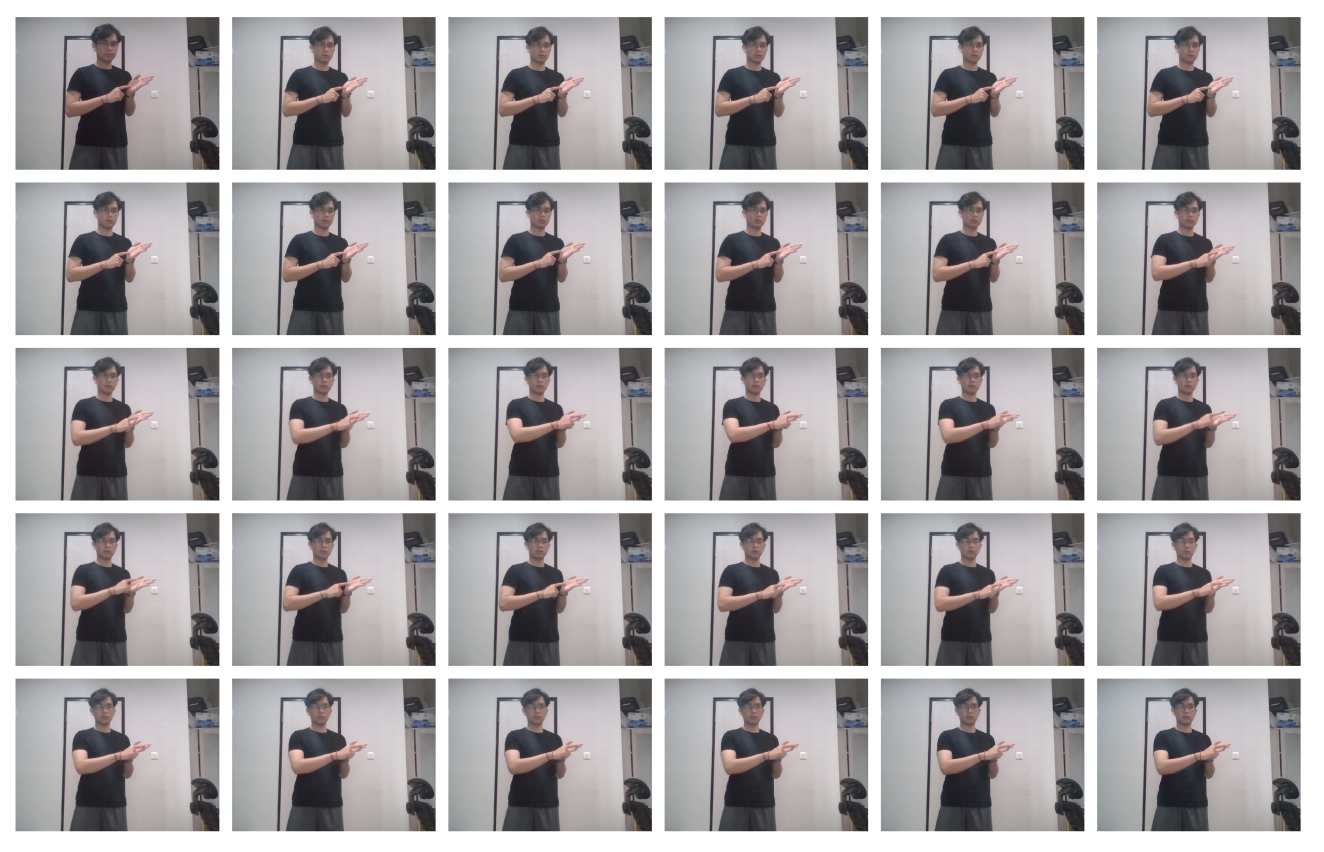
\includegraphics[scale=0.35]{gambar/isyarat-clear-nama.png}

  \caption{Dataset kosakata "nama"}
  \label{fig:datasetMethod}
\end{figure}

Adapun bahasa isyarat yang akan digunakan pada tugas akhir ini meliputi 6 kosakata isyarat BISINDO yang memiliki konteks kalimat yang umum digunakan sehari – hari. Nantinya untuk setiap kosakata tersebut akan disimpan sebanyak 30 jumlah data dengan masing - masing data terkumpul sebanyak 30 \emph{frame}. Kosakata yang akan digunakan adalah sebagai berikut:

\begin{longtable}{|c|c|c|c|}
  \caption{Kosakata BISINDO}
  \label{tb:kosakataBISINDO}                                   \\
  \hline
  \rowcolor[HTML]{C0C0C0}
  \textbf{No} & \textbf{Kelas} & \textbf{Jumlah Data} & \textbf{Jumlah \emph{Frame}}\\
  \hline
  1            & Maaf                       & 30            & 30\\
  2            & Tolong                     & 30            & 30\\
  3            & Saya                       & 30            & 30\\
  4            & Nama                       & 30            & 30\\
  5            & Rumah                       & 30            & 30\\
  6            & Siapa                       & 30            & 30\\
  \hline
\end{longtable}

% Digunakan tambahan 3 buah isyarat tambahan di luar isyarat BISINDO untuk mempermudah kontrol sistem penerjemah. Isyarat tersebut meliputi isyarat mulai (\textit{start}), isyarat \textit{standby}, isyarat hapus kata (\textit{delete}), dan isyarat terjemah (\textit{translate}).  

Dalam mempermudah kontrol sistem penerjemah, digunakan 3 gerakan isyarat tambahan di luar gerakan isyarat BISINDO.  Isyarat tersebut meliputi isyarat \textit{standby}, isyarat hapus kata (\textit{delete}), dan isyarat terjemah menjadi suara (\textit{translate}).  Untuk setiap gerakan isyarat kontrol juga memiliki jumlah data yang sama dengan gerakan isyarat BISINDO, yaitu 30 data dengan 30 \emph{frame} pada setiap datanya.

\begin{longtable}{|c|c|c|c|}
  \caption{Isyarat Kontrol Tambahan}
  \label{tb:isyaratkontrol}                                   \\
  \hline
  \rowcolor[HTML]{C0C0C0}
  \textbf{No} & \textbf{Kelas} & \textbf{Jumlah Data} & \textbf{Jumlah \emph{Frame}}\\
  \hline
  1            & \textit{Standby}                       & 30             & 30 \\
  2            & \textit{Translate}                     & 30             & 30 \\
  3            & \textit{Delete}                        & 30             & 30 \\
  \hline
\end{longtable}

\subsection{Estimasi Pose}

\begin{figure}[H]
  \centering

  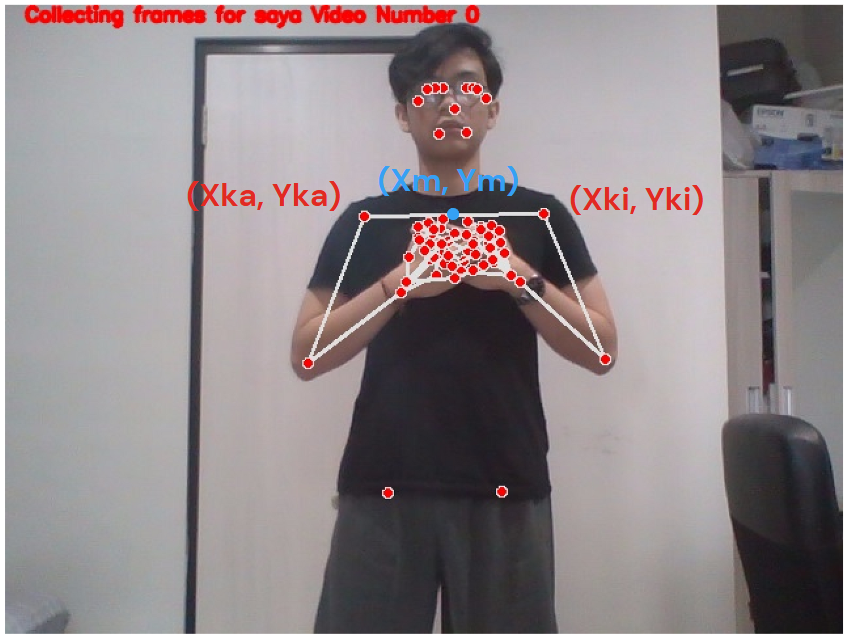
\includegraphics[scale=0.6]{gambar/bab3-estimasi-pose.png}

  \caption{Estimasi pose pada citra}
  \label{fig:poseEstimationMethod}
\end{figure}

Untuk setiap citra pada 30 data yang telah dilakukan estimasi pose dengan bantuan \textit{framework} MediaPipe. \textit{Framework} ini dapat melacak titik – titik bagian tubuh atau \textit{landmark} menggunakan model yang disediakan. Model MediaPipe yang akan digunakan adalah MediaPipe pose dan MediaPipe hand. Dalam pembentukan isyarat BISINDO, bagian tubuh yang bergerak adalah bagian tangan dan lengan. Melalui MediaPipe hand akan dilakukan ekstraksi untuk 21 \textit{landmark} pada bagian tangan, sehingga total \textit{landmark} untuk tangan kanan dan kiri adalah 42 \textit{landmark}. Kemudian melalui MediaPipe pose akan dilakukan ekstraksi pada bagian bahu sampai lengan sehingga \textit{landmark} yang akan digunakan hanya pada posisi 11 hingga 22 sehingga total \textit{landmark} untuk bagian tubuh adalah 12 \textit{landmark}. Untuk setiap \textit{landmark} yang didapatkan akan digunakan koordinat x dan y saja (koordinat z dan \textit{visibility} tidak digunakan). Hal ini berguna demi menghasilkan model akhir yang memiliki kemampuan untuk invarian terhadap skala (jarak kamera tidak mempengaruhi estimasi pose) dan invarian terhadap rotasi (adanya rotasi tidak mempengaruhi koordinat yang digunakan). Hal ini juga dilakukan demi melakukan reduksi dimensi sehingga mengurangi resiko \textit{overfitting} dan dapat mempercepat performa model. Nantinya, untuk setiap citra yang akan diproses pada MediaPipe akan menghasilkan total 42 koordinat dari \textit{landmark} tangan kanan, 42 koordinat dari \textit{landmark} tangan kiri, dan 24 koordinat dari \textit{landmark} pose.Hal ini dapat dilihat pada gambar \ref{fig:poseEstimationMethod}, \textit{landmark} yang akan digunakan hanyalah \textit{landmark} yang saling terhubung (ditandai dengan garis putih). Sedangkan \textit{landmark} yang hanya berbentuk titik saja tidak akan digunakan dan tidak akan diambil data koordinatnya. Data koordinat \textit{landmark} yang berbentuk array multidimensi kemudian akan diproses melalui \textit{library} Numpy dengan menggunakan fungsi concatenate menjadi satu dimensi saja untuk mempermudah pada klasifikasi pose pada tahap \textit{training} data.

\subsubsection{Normalisasi Data}
Keseluruhan data koordinat yang didapatkan melalui estimasi pose menggunakan MediaPipe akan melalui proses normalisasi. Normalisasi data dilakukan demi mengatasi adanya \textit{scale invariant} dan \textit{position invariant}. \textit{Scale invariant} dalam konteks tugas akhir ini adalah kemampuan model dalam mengklasifikasikan data bahasa isyarat yang dilakukan oleh berbagai macam pengguna yang memiliki bentuk tubuh yang berbeda - beda. Selain itu, \textit{scale invariant} juga menyebabkan jarak pengguna dengan kamera tidak mempengaruhi proses klasifikasi model. \textit{Position invariant} dalam konteks tugas akhir ini adalah kemampuan model dalam mengklasifikasikan data bahasa isyarat dalam berbagai posisi pengguna terhadap kamera (dengan catatan bahwa posisi tangan dan bahu dapat terlihat jelas ketika pengguna melakukan gerakan isyarat).

\begin{equation}
  \label{eq:shouderWidthNorm}
  w = \sqrt{(x_{ka} - x_{ki})^2 + (y_{ka} - y_{ki})^2}
\end{equation}

\begin{equation}
  \label{eq:shoulderMidpointNorm}
  x_m = \frac{x_{ka} + x_{ki}}{2} ; \\
   y_m = \frac{y_{ka} + y_{ki}}{2}
\end{equation}

\begin{equation}
  \label{eq:normalization}
  x'_i = \frac{x_i - x_m}{w} ;  \\
   y'_i = \frac{y_i - y_m}{w}
\end{equation}

Dalam melakukan proses normalisasi, terlebih dahulu didapatkan panjang dari bahu dengan menggunakan rumus jarak \textit{Euclidian}. Rumus ini akan menghitung kuadrat selisih antara koordinat x dan y antara \textit{landmark} bahu kanan dan kiri. Hasil dari kedua operasi tersebut kemudian dijumlahkan dan dihitung akar kuadratnya. Perhitungan jarak \textit{Euclidian} dapat dapat dilihat pada rumus \ref{eq:shouderWidthNorm}. Untuk mendapatkan titik tengah dari \textit{landmark} bahu, dilakukan dengan menjumlahkan masing - masing koordinat x dan y dari bahu kanan dan kiri, kemudian dibagi dengan 2. Proses ini dapat dilihat pada rumus \ref{eq:shoulderMidpointNorm}.

Normalisasi data akan dilakukan dengan melakukan pengurangan terhadap setiap koordinat \textit{landmark} dengan koordinat titik tengah dari bahu dan diakhiri dengan pembagian dengan panjang dari bahu yang telah dihitung sebelumnya. Hal ini dapat dilihat pada rumus \ref{eq:normalization}. Perlu diketahui bahwa pada perumusan diatas, $w$ adalah panjang bahu, $x_{ka}$ adalah koordinat x bahu kanan, $y_{ka}$ adalah kooridnat y bahu kanan, $x_{ki}$ adalah koordinat x bahu kiri, $y_{ki}$ adalah kooridnat y bahu kiri, $x'_i$ adalah koordinat x yang telah dinormalisasi, dan $y'_i$ adalah kooridnat y yang telah dinormalisasi.

Nantinya data koordinat yang telah dinormalisasi ini akan disimpan dalam bentuk array dengan bantuan Numpy dan akan digunakan dalam proses \textit{training}. Normalisasi data tidak hanya digunakan dalam proses pembuatan model, tetapi juga nantinya dalam proses klasifikasi bahasa isyarat dengan menggunakan model. Hal ini dilakukan sehingga koordinat - kooridnat yang diproses adalah homogen dan menghindari adanya \textit{noise} atau \textit{error}.

\subsection{Klasifikasi Pose}
\label{sec:metodologipose}

Dalam melakukan klasifikasi terhadap pose atau gerakana isyarat yang dilakukan, digunakan model LSTM dengan bentuk sekuensial sehingga dapat menggabungkan serangkaian \emph{layer} untuk menghasilkan model penerjemah bahasa isyarat yang memiliki performa baik. \emph{Layer} pertama merupakan \emph{layer} \textit{TimeDistributed} yang di dalamnya terdapat \emph{layer} \textit{Dense} dengan jumlah unit sebesar 128, fungsi aktivasi '\textit{tanh}' dan input dengan bentuk (30, 108). Penggunaan \textit{TimeDistributed} memastikan bahwa untuk setiap frame akan diproses secara independen, dimana diimplementasikan \emph{layer} \textit{Dense} yang konsisten pada setiap frame yang ada. Perlu diperhatikan bentuk data (30, 108) berarti akan terdapat 30 jumlah frame, dimana untuk setiap frame akan diekstrak total 108 fitur. 108 fitur tersebut merupakan kumpulan dari data koordinat x dan y untuk setiap \emph{landmark} Mediapipe yang digunakan.\emph{Layer} kedua merupakan LSTM pertama yang memiliki jumlah unit 128, return\_sequences=True, fungsi aktivasi '\textit{tanh}', dan input dalam bentuk (30, 108). Pada \emph{layer} ketiga diikuti dengan \emph{layer} Dropout dengan nilai 0.5 untuk menghindari adanya nilai \emph{weight} yang terlalu tinggi. \emph{Layer} selanjutnya, yaitu \emph{layer} keempat merupakan layer LSTM kedua yang memiliki jumlah unit 128, return\_sequences=False, dan fungsi aktivasi '\textit{tanh}'. Pada \emph{layer} kelimat diikuti dengan \emph{layer} Dropout dengan nilai 0.5 untuk menghindari adanya nilai \emph{weight} yang terlalu tinggi. Dapat dilihat bahwa untuk setiap \emph{layer} LSTM memiliki \emph{layer} Dropout untuk menghindari \emph{overfitting} pada model dengan menonaktifkan \emph{neuron} dengan probabilitas sebesar 50\%. 

Untuk menyederhanakan kompleksitas dari data output yang diberikan 2 layer LSTM, digunakan \emph{layer} Dense dengan jumlah unit 128 dan fungsi aktivasi 'relu'. Setelah \emph{layer} \textit{Dense}, diberikan \emph{layer} Dropout dengan nilai 0.2 untuk menghindari adanya kelebihan \emph{overfitting} pada model. \emph{Layer} terakhir adalah \emph{layer} \textit{Dense} yang menggunakan fungsi aktivasi '\textit{softmax}'. Jumlah unit di \emph{layer} ini sesuai dengan actions.shape[0], yang berarti jumlah unit sama dengan jumlah aksi atau kategori yang mungkin. Fungsi aktivasi '\textit{softmax}' memastikan bahwa keluaran dari model ini adalah distribusi probabilitas di atas semua kategori yang mungkin, dengan total semua probabilitas sama dengan 1. Model ini kemudian dikompilasi menggunakan \emph{optimizer} Adam, yang dikenal karena performa dan efisiensinya dalam pelatihan jaringan saraf, dan menggunakan \textit{categorical crossentropy} sebagai fungsi \textit{loss} karena ini adalah masalah klasifikasi multi-kelas, dengan metrik akurasi kategorikal untuk memantau performa model selama proses \textit{training}. 

\begin{figure}[H]
  \centering

  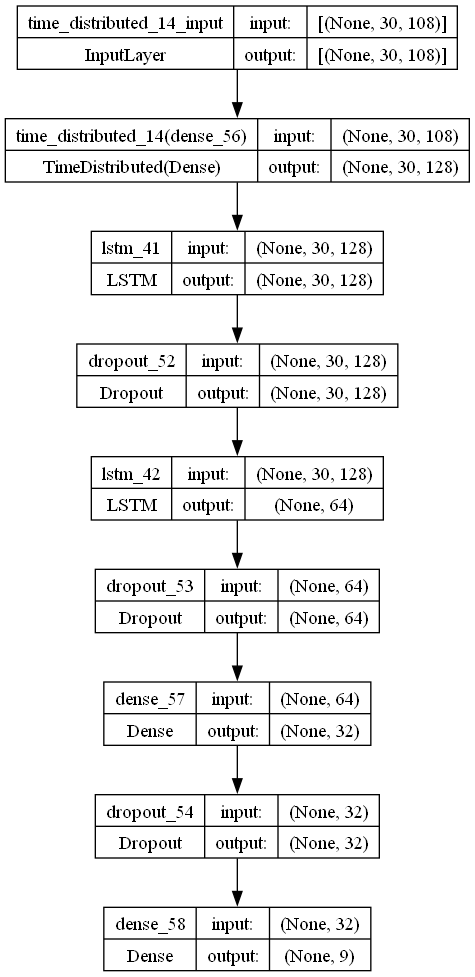
\includegraphics[scale=0.5]{gambar/bab4-uji-model-best-model.png}

  \caption{Model LSTM}
  \label{fig:modelLSTM}
\end{figure}

\subsection{Sistem Kontrol}
\label{sec:metodologisistemkontrol}

Adapun dalam pembuatan tugas akhir ini, sistem kontrol adalah serangkaian proses yang akan mengatur bagaimana nantinya bahasa isyarat akan dideteksi, melakukan penanggulangan terhadap adanya kesalahan pendeteksian, menyatukan berbagai kata dalam bentuk kalimat, penghapusan kosakata, dan penerjemahan kalimat dalam bentuk suara. Penggunaan sistem kontrol ini diharapkan akan memudahkan pengguna dalam menggunakan program penerjemah bahasa isyarat Indonesia (BISINDO). Sistem kontrol akan dibagi menjadi 2, yaitu program deteksi bahasa isyarat dan program pembentukan kalimat.

\subsubsection{Program Deteksi Bahasa Isyarat}

\begin{figure}[H]
  \centering

  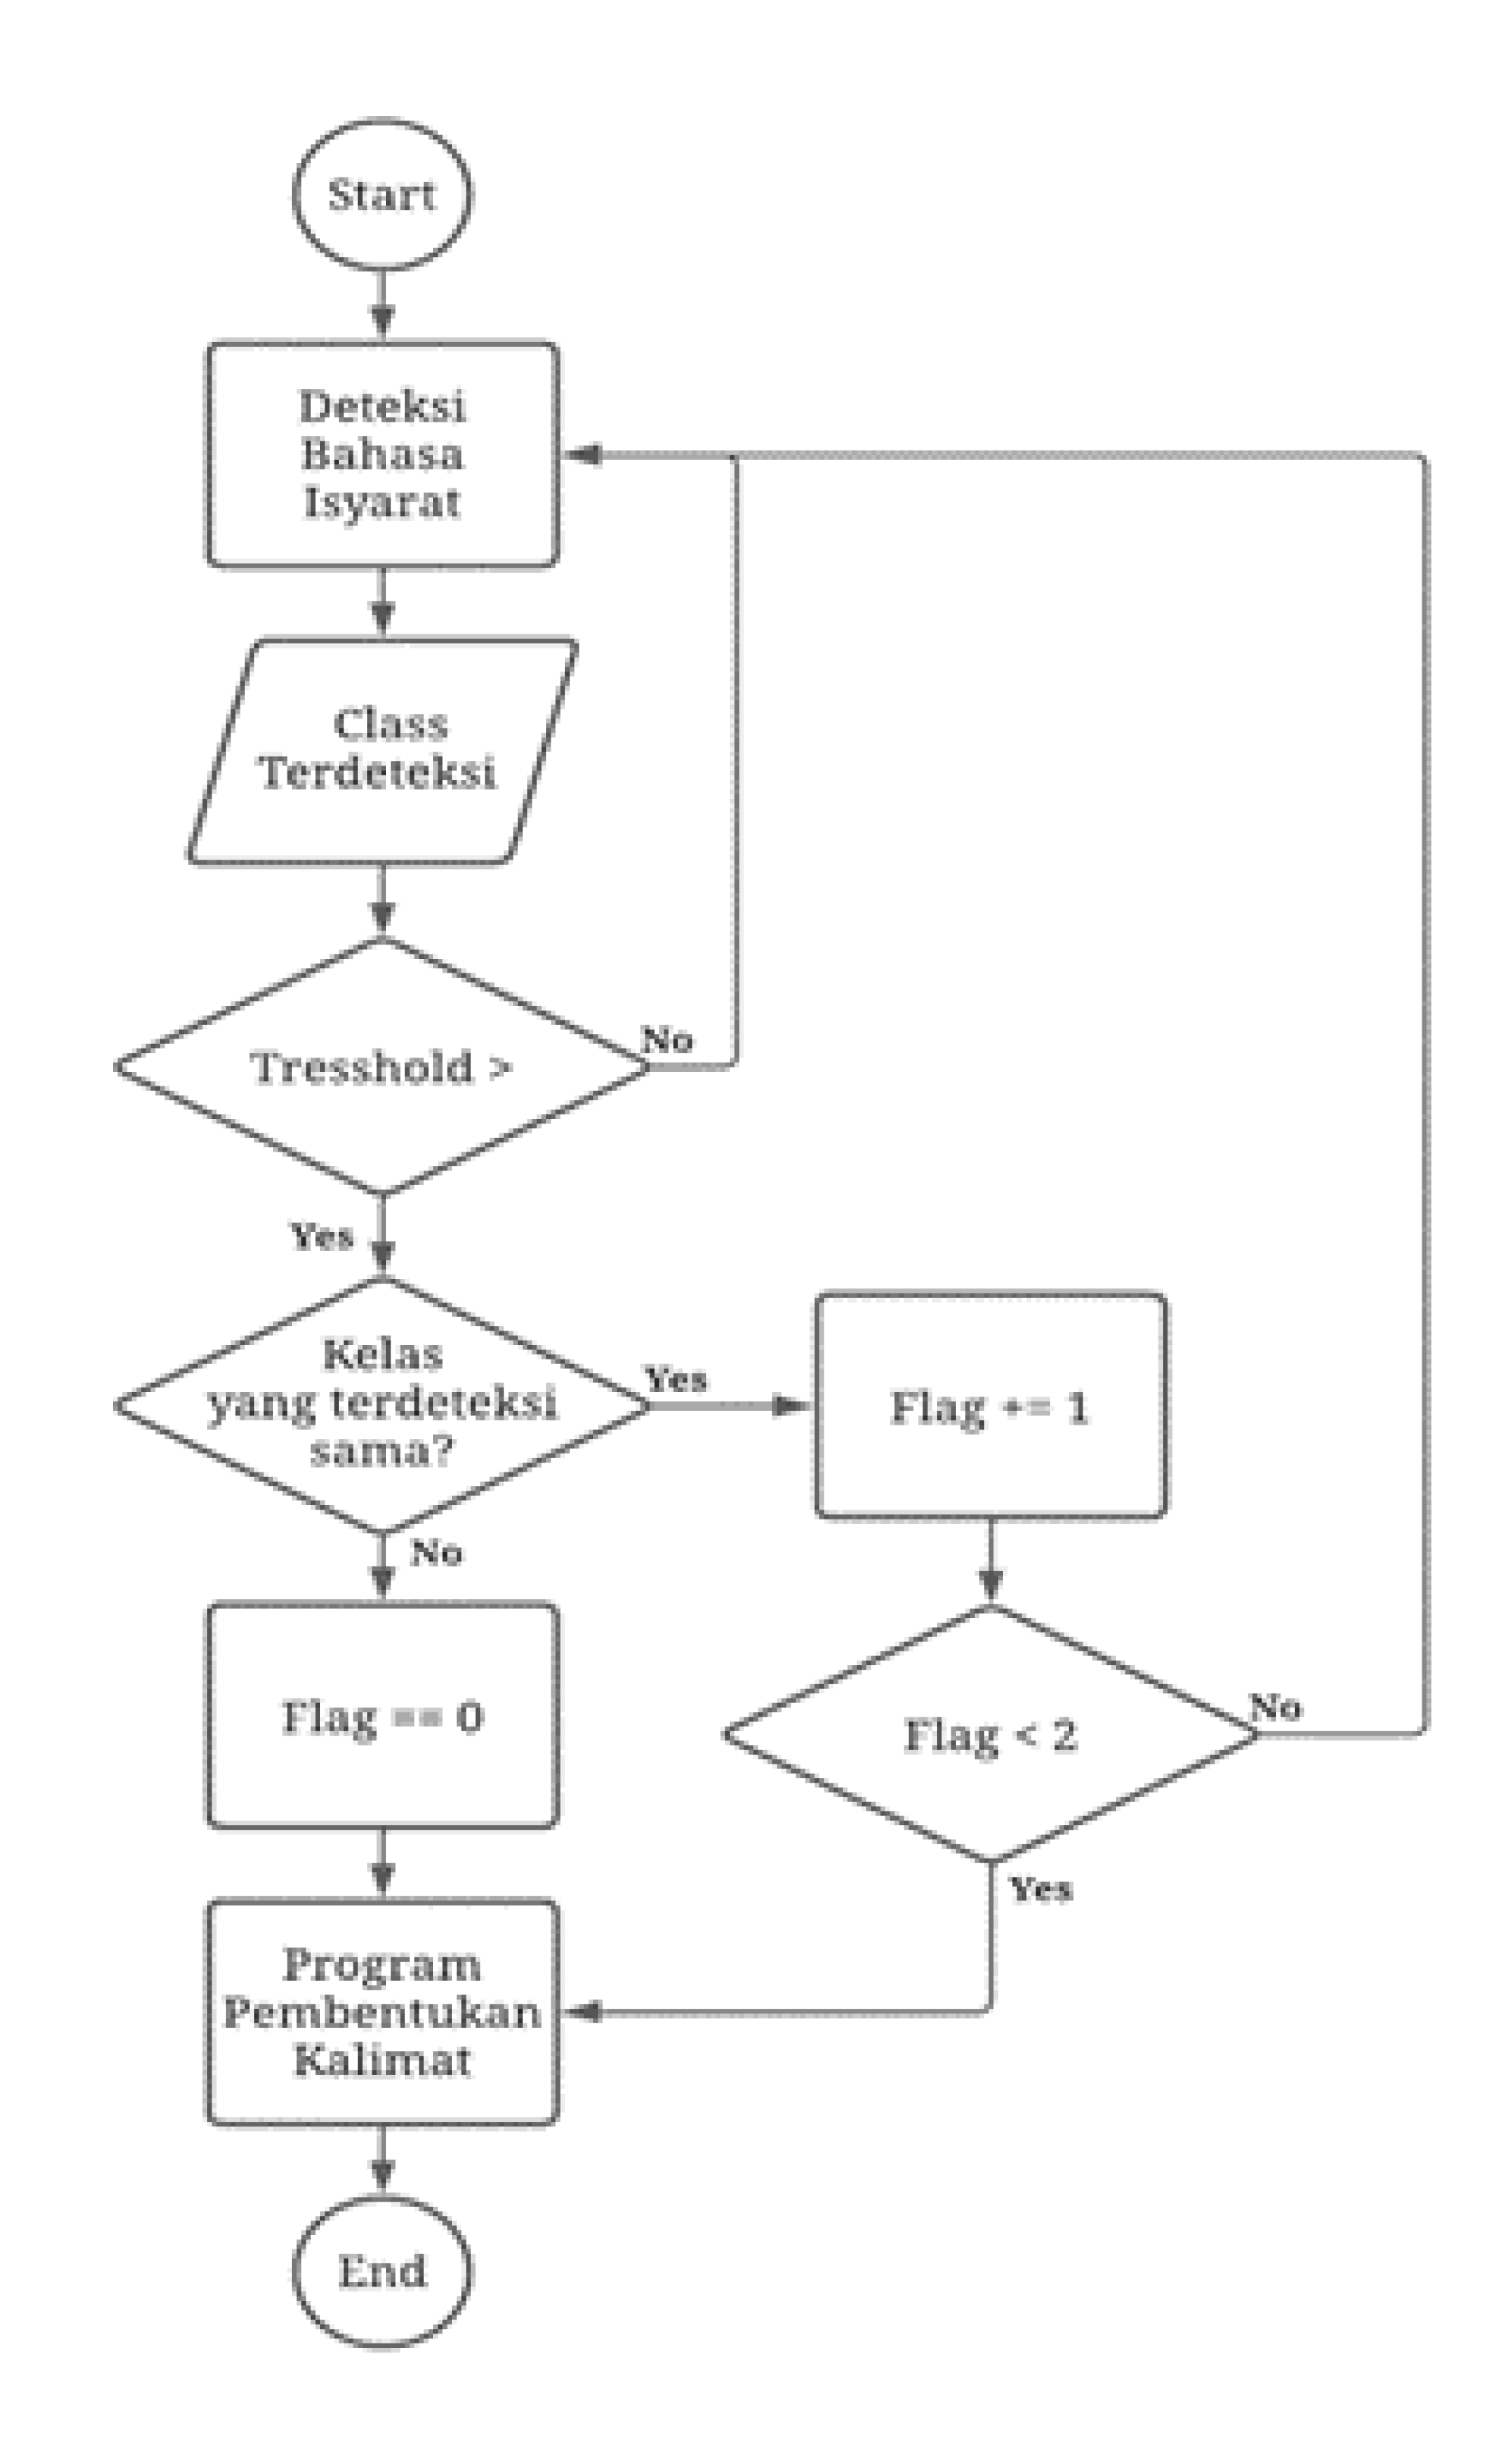
\includegraphics[scale=0.54]{gambar/bab3-flowchart-deteksi.png}

  \caption{Flowchart program deteksi bahasa isyarat}
  \label{fig:flowchartdeteksi}
\end{figure}
Pada program deteksi bahasa isyarat (dapat dilihat pada \ref{fig:flowchartdeteksi}) akan berjalan terlebih dahulu ketika pengguna terdeteksi benar memberikan isyarat start dan pengguna dapat membentuk isyarat yang diinginkan. Kemudian \textit{class} kosakata isyarat yang terdeteksi oleh model akan dipastikan apakah melebihi \textit{threshold} atau ambang batas yang telah ditentukan untuk menghindari adanya kesalahan pembacaan (\textit{error}) dan \textit{noise} dalam pembacaan bahasa isyarat. Apabila dibawah dari \textit{threshold}, maka program akan melakukan pendeteksian kembali bahasa isyarat dari pengguna. Apabila benar diatas dari \textit{threshold} yang ditentukan, maka akan diperiksa apakah \textit{class} yang terdeteksi sama dengan \textit{class} sebelumnya. Apabila terdeteksi sama maka nilai \textit{flag} akan ditambah 1. Nilai \textit{flag} akan diperiksa apakah kurang dari 2, apabila salah maka akan kembali untuk mendeteksi bahasa isyarat dari pengguna. Hal ini dilakukan demi menghindari terjadinya pembacaan isyarat secara berulang kali. Apabila nilai \textit{flag} bernilai 1 atau 0 (nilai awal \textit{flag} adalah 0), maka akan dilanjutkan ke program pembentukan kalimat.

\subsubsection{Program Pembentuk Kalimat}
\begin{figure}[H]
  \centering

  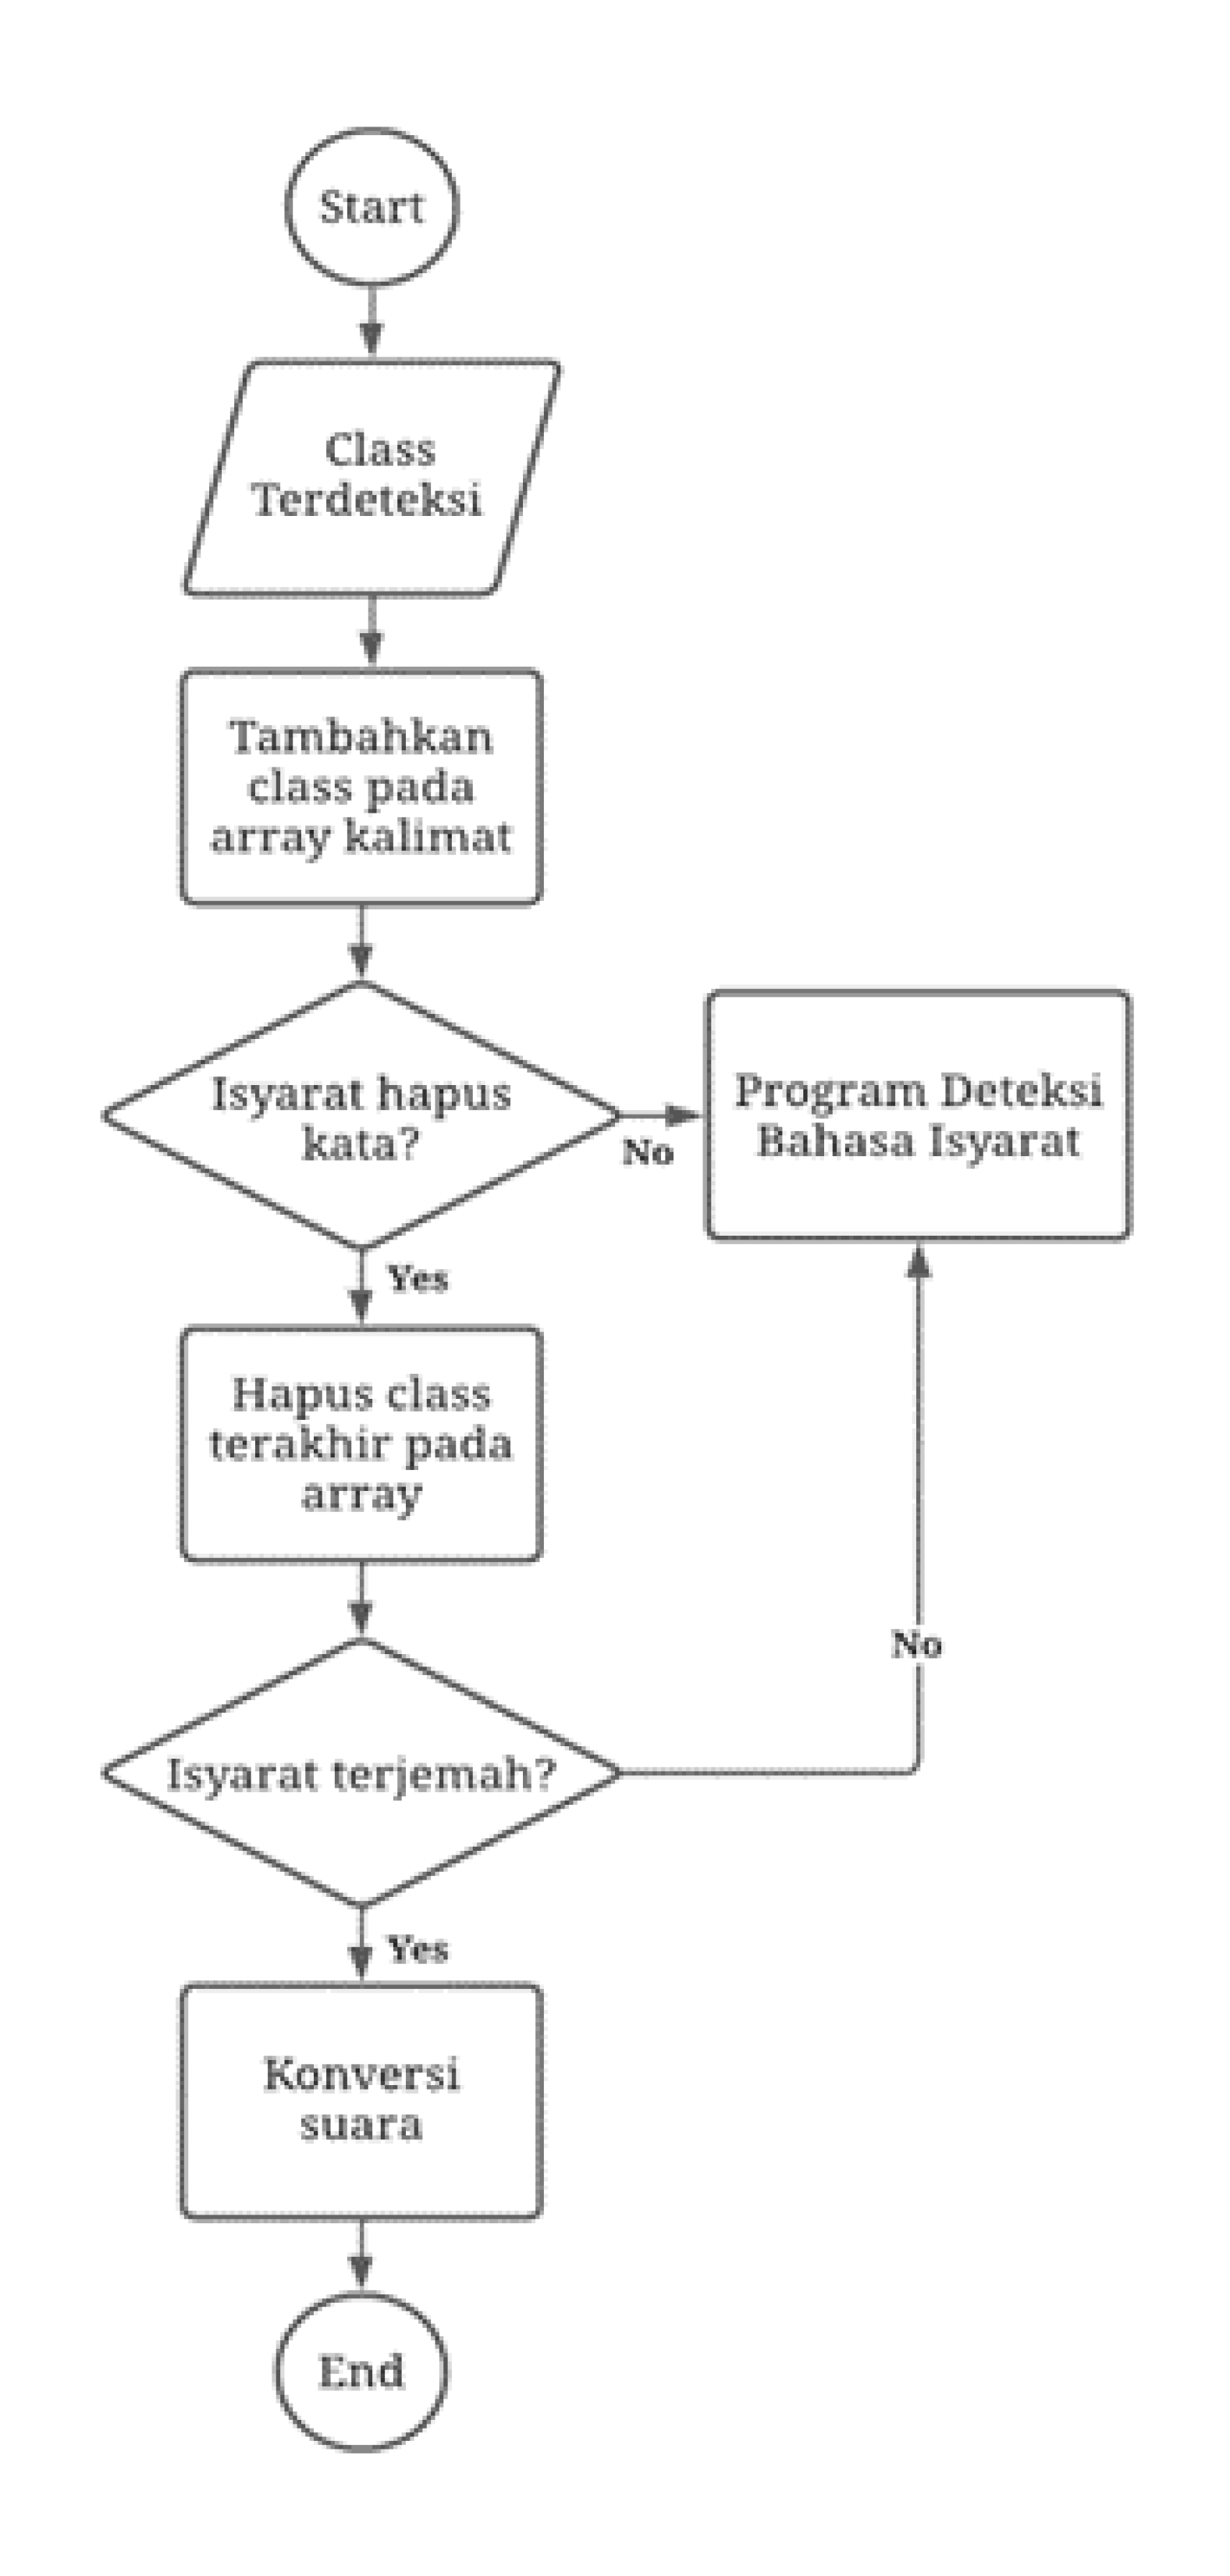
\includegraphics[scale=0.54]{gambar/bab3-flowchart-kalimat.png}

  \caption{Flowchart Program pembentukan kalimat}
  \label{fig:flowchartkalimat}
\end{figure}

Pada program pembentukan kalimat (dapat dilihat pada \ref{fig:flowchartkalimat}), terlebih dahulu \textit{class} kosakata yang terdeteksi akan dimasukkan pada suatu array kalimat dan ditambahkan spasi setelahnya. Hal ini nantinya akan memudahkan pengguna dalam membentuk kalimat yang diinginkan. Kemudian dilakukan pengecekan apakah pengguna melakukan isyarat delete atau hapus, apabila iya maka akan dilakukan penghapusan pada kata terakhir pada array. Apabila tidak maka akan dilanjutkan untuk melakukan pendeteksian bahasa isyarat selanjutnya. Dilakukan juga pengecekan apakah terdapat isyarat translate atau isyarat terjemah, jika iya maka akan dilakukan konversi dari array kalimat yang telah disimpan ke dalam suara dengan memanfaatkan \textit{library} gTTS. Library gTTS merupakan \textit{library} Python yang memiliki kemampuan untuk mengubah suatu string menjadi suara. Nantinya akan dipilih suara dengan aksen Indonesia untuk meningkatkan familiaritas terhadap lingkungan sekitar. Apabila tidak maka akan dilanjutkan untuk melakukan pendeteksian bahasa isyarat selanjutnya.

\subsection{Integrasi Intel Next Unit Computing (NUC)}
\begin{figure}[H]
  \centering

  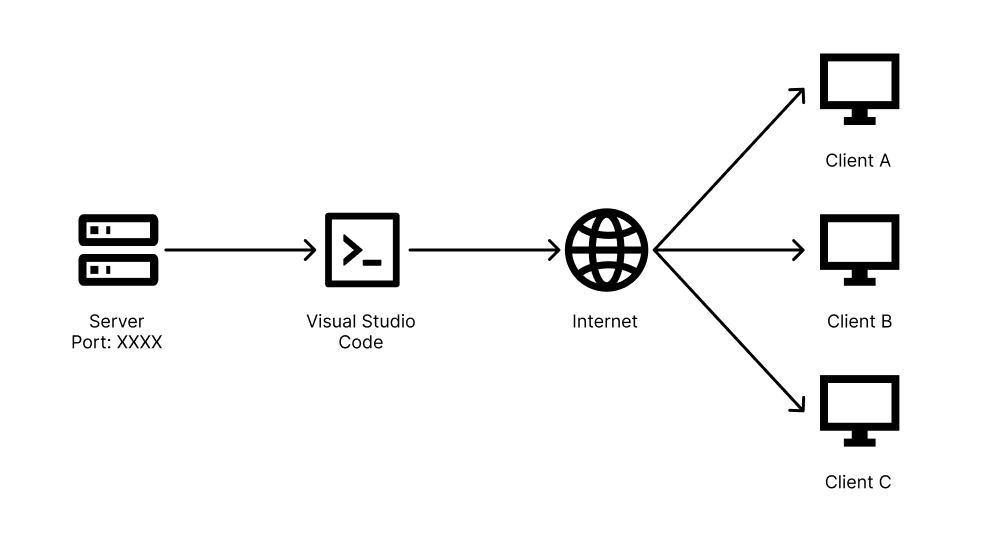
\includegraphics[scale=0.9]{gambar/bab3-path-forwarding.png}

  \caption{Skema integrasi dengan Intel NUC}
  \label{fig:diagrampathforward}
\end{figure}

Sebelum melakukan integrasi, terlebih dahulu perangkat dihubungkan dengan perangkat pendukung seperti monitor, keyboard, mouse, dan speaker. Kemudian, integrasi dengan Intel NUC dilakukan dengan mengakses website penerjemah yang telah terhubung dengan server komputer menggunakan skema \emph{port forwarding} dengan diagram alur yang dapat dilihat pada \ref{fig:blockdiagrammethod}. Server terelebih dahulu mengakses Visual Studio Code untuk menjalankan website penerjemah yang dibuat menggunakan \emph{framework} Streamlit. Akan didapatkan alamat untuk mengakses website tersebut secara lokal (\emph{localhost}), dimana nilai port yang dimiliki oleh server akan diteruskan (\emph{forwarding}) dengan bantuan Ngrok sehingga nantinya akan dapat diakses melalui internet dengan bebas oleh client, yang mana dalam hal ini adalah Intel NUC itu sendiri.

Dapat dilihat pada gambar \ref{fig:tampilanwebsite} bahwa website penerjemah akan mengakses webcam perang\\kat untuk mendapatkan data citra berbentuk video secara \emph{realtime}. Pengguna kemudian dapat melakukan gerakan bahasa isyarat BISINDO di depan webcam. Website penerjemah akan mengekstrak data citra untuk diproses melalui model LSTM yang telah dilatih sebelumnya dan melakukan penerjemahan secara \emph{realtime} sesuai dengan alur program yang telah dijelaskan sebelumnya pada sub bab \ref{sec:metodologisistemkontrol}. 

\begin{figure}[H]
  \centering

  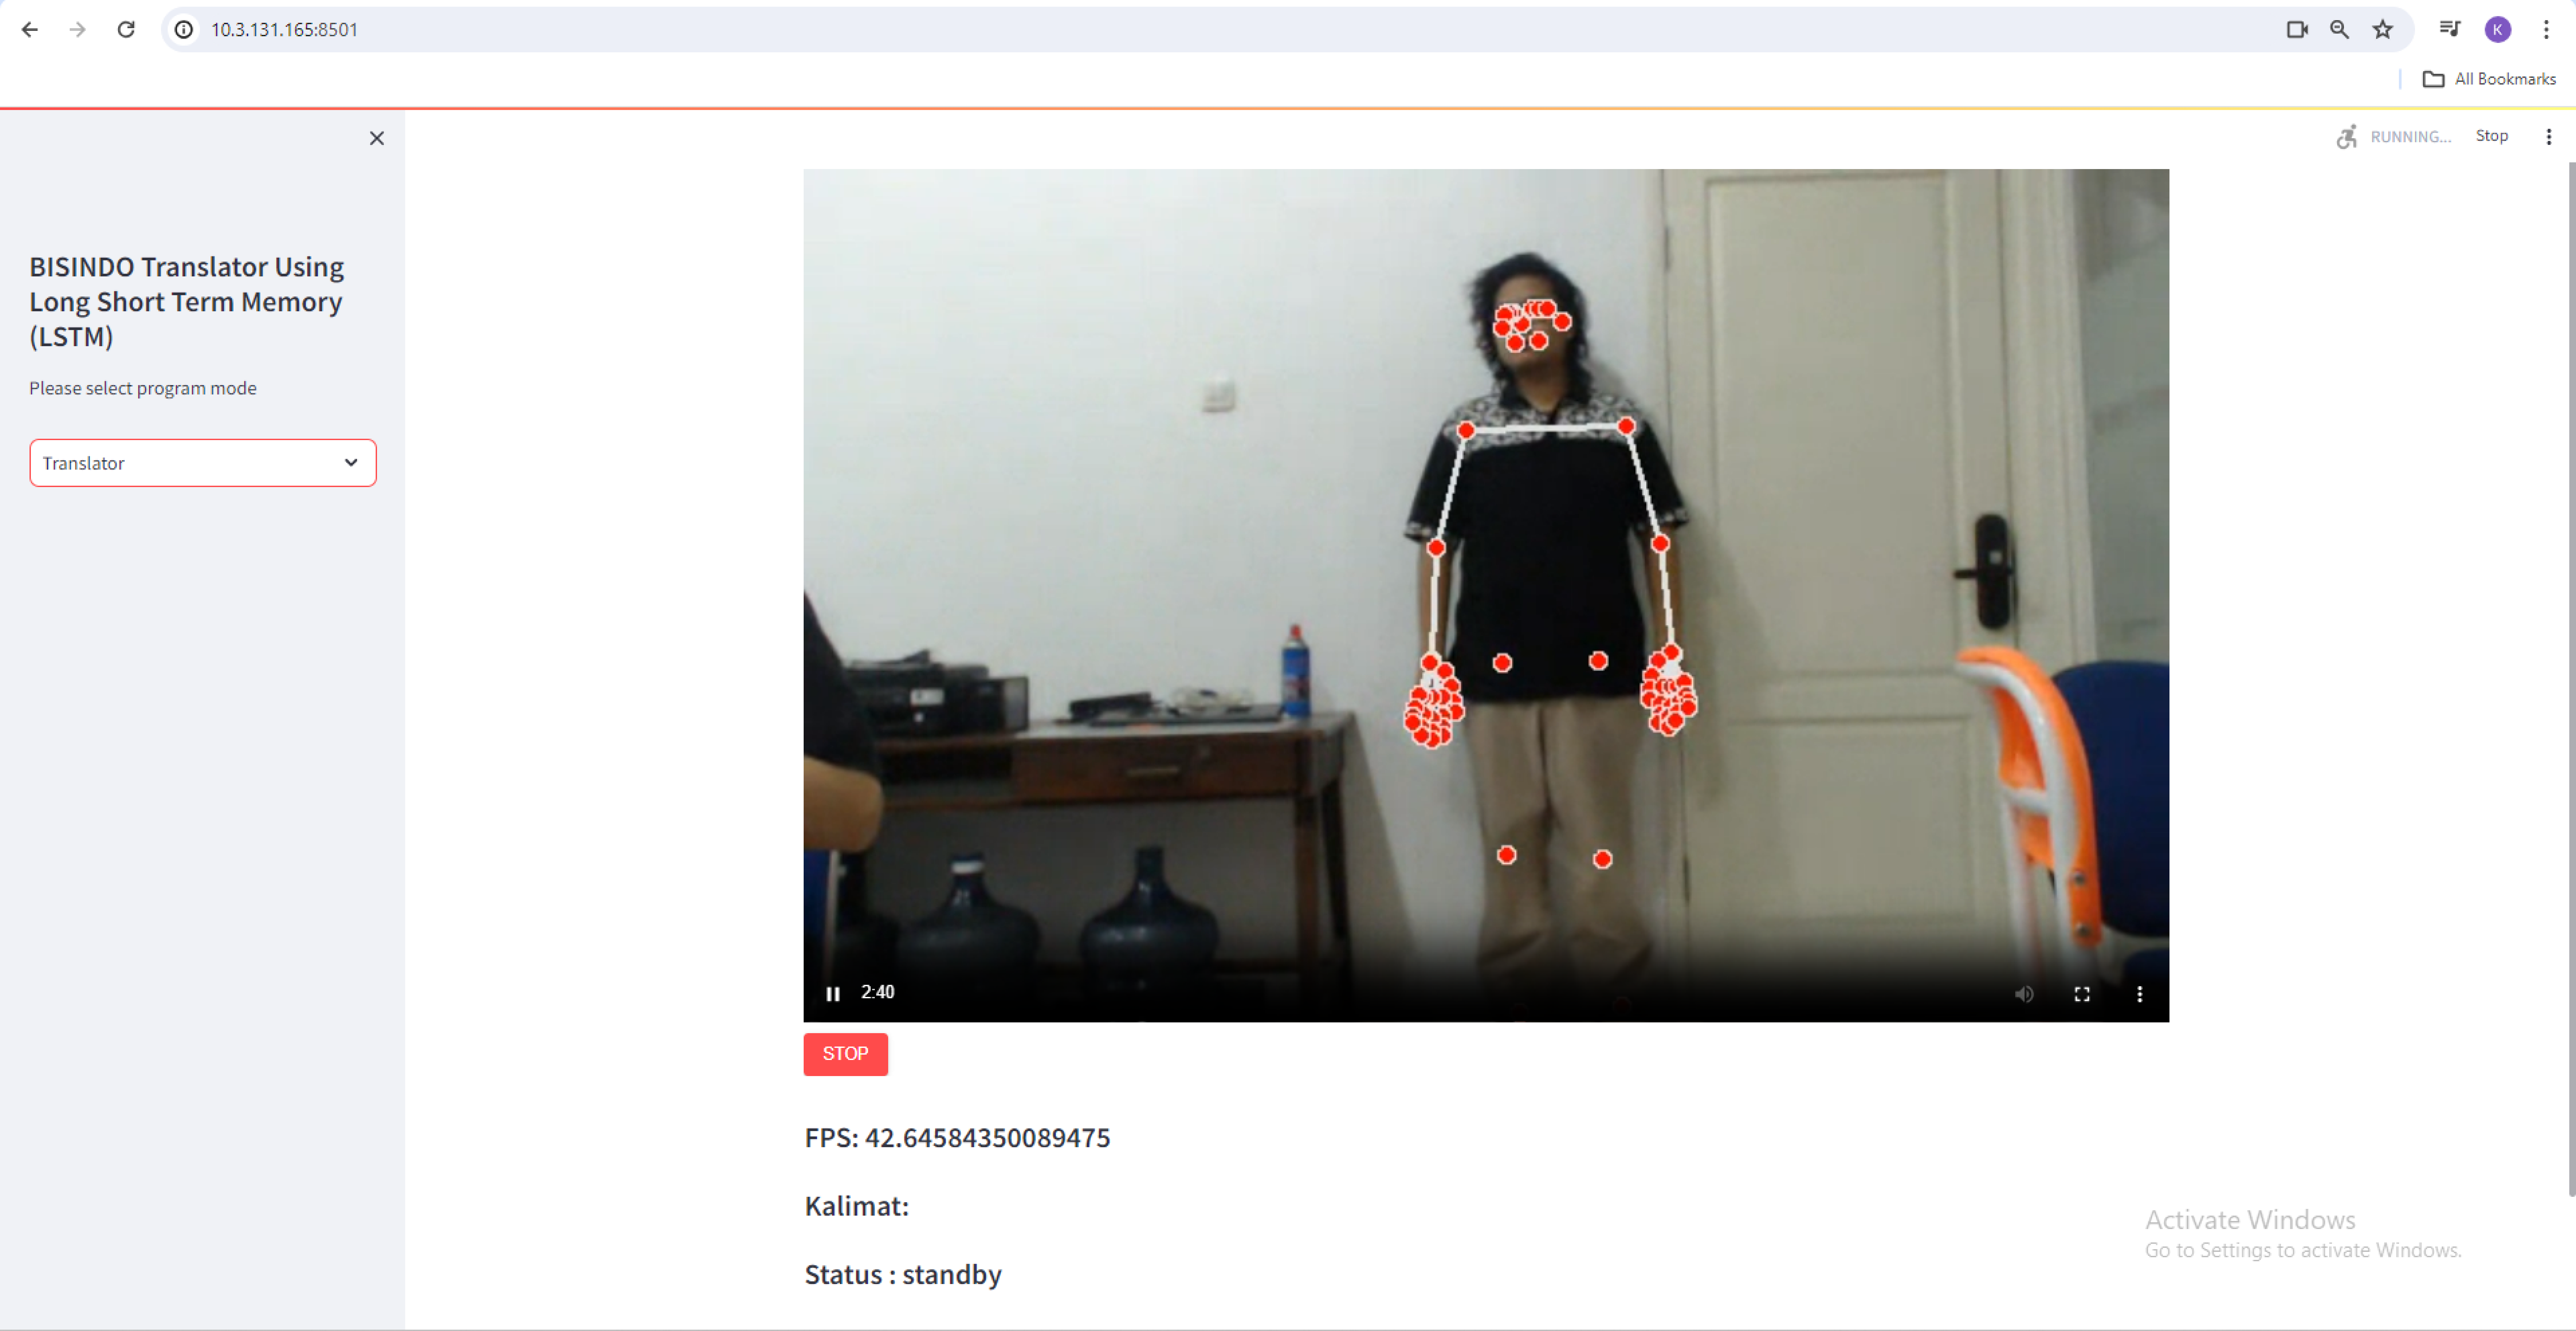
\includegraphics[scale=0.2]{gambar/bab3-layoutweb.png}

  \caption{Tampilan website}
  \label{fig:tampilanwebsite}
\end{figure}


% \subsection{Integrasi Jetson Nano}

% Sebelum dapat menggunakan Jetson Nano, terlebih dahulu mengunuh dan mengingstall NVIDIA JetPack SDK yang mencakup sistem operasi, \textit{library}, API, dan driver yang diperlukan. Proses ini melibatkan penggunaan aplikasi SDK Manager yang menyediakan antarmuka pengguna grafis untuk memudahkan penginstalan dan setup. Selanjutnya, konfigurasi perangkat keras Jetson Nano, termasuk menyediakan sumber daya listrik yang stabil, menghubungkan perangkat ke monitor melalui port HDMI, serta menyiapkan periferal lain seperti keyboard dan mouse. Untuk pengembangan yang melibatkan pengolahan citra atau video, kamera yang kompatibel juga perlu dihubungkan dan dikonfigurasi. Oleh karena Jetson Nano tidak memiliki port audio, maka digunakan USB dongle untuk dapat menyambungkan Jetson Nano dengan speaker. Kemudian dilakukan instalasi untuk setiap dependency atau \textit{library} yang dibutuhkan, seperti Python, Jupyter, TensorFlow, Keras, Pytorch, MediaPipe, Numpy, Maplotlib, dan \textit{library} lainnya. Untuk dapat menunjang performa dari Jetson Nano dalam menjalankan program, terkhususnya model penerjemah bahasa isyarat, dilakukan instalasi dan setup untuk CUDA (\textit{Compute Unified Device Architecture}) sehingga Jetson Nano dapat menggunakan GPU (\textit{Graphic Processing Unit}). 

% Untuk melakukan deploy program pendeteksi bahasa isyarat pada Jetson Nano, pada model yang telah dihasilkan sebelumnya dilakukan optimasi dengan melakukan konversi menggunakan TensorRT dan kuantisasi. Hal ini dimaksudkan untuk mengoptimalkan performa model pada Jetson Nano. Kemudian program sistem penerjemah bahasa isyarat (dalam bentuk python executable) dapat ditransfer ke Jetson Nano dengan menggunakan Git. Program siap melakukan penerjemahan bahasa isyarat BISINDO.

% \section{Urutan Pelaksanaan}

% Adapun dalam pembuatan tugas akhir ini, berikut urutan pelaksanaan penelitian yang akan dilakukan oleh penulis:

% \begin{figure}[H]
%   \centering
%   \caption{Flowchart Program Pembentukan Kalimat}
%   \label{tbl:flowchartkalimat}

%   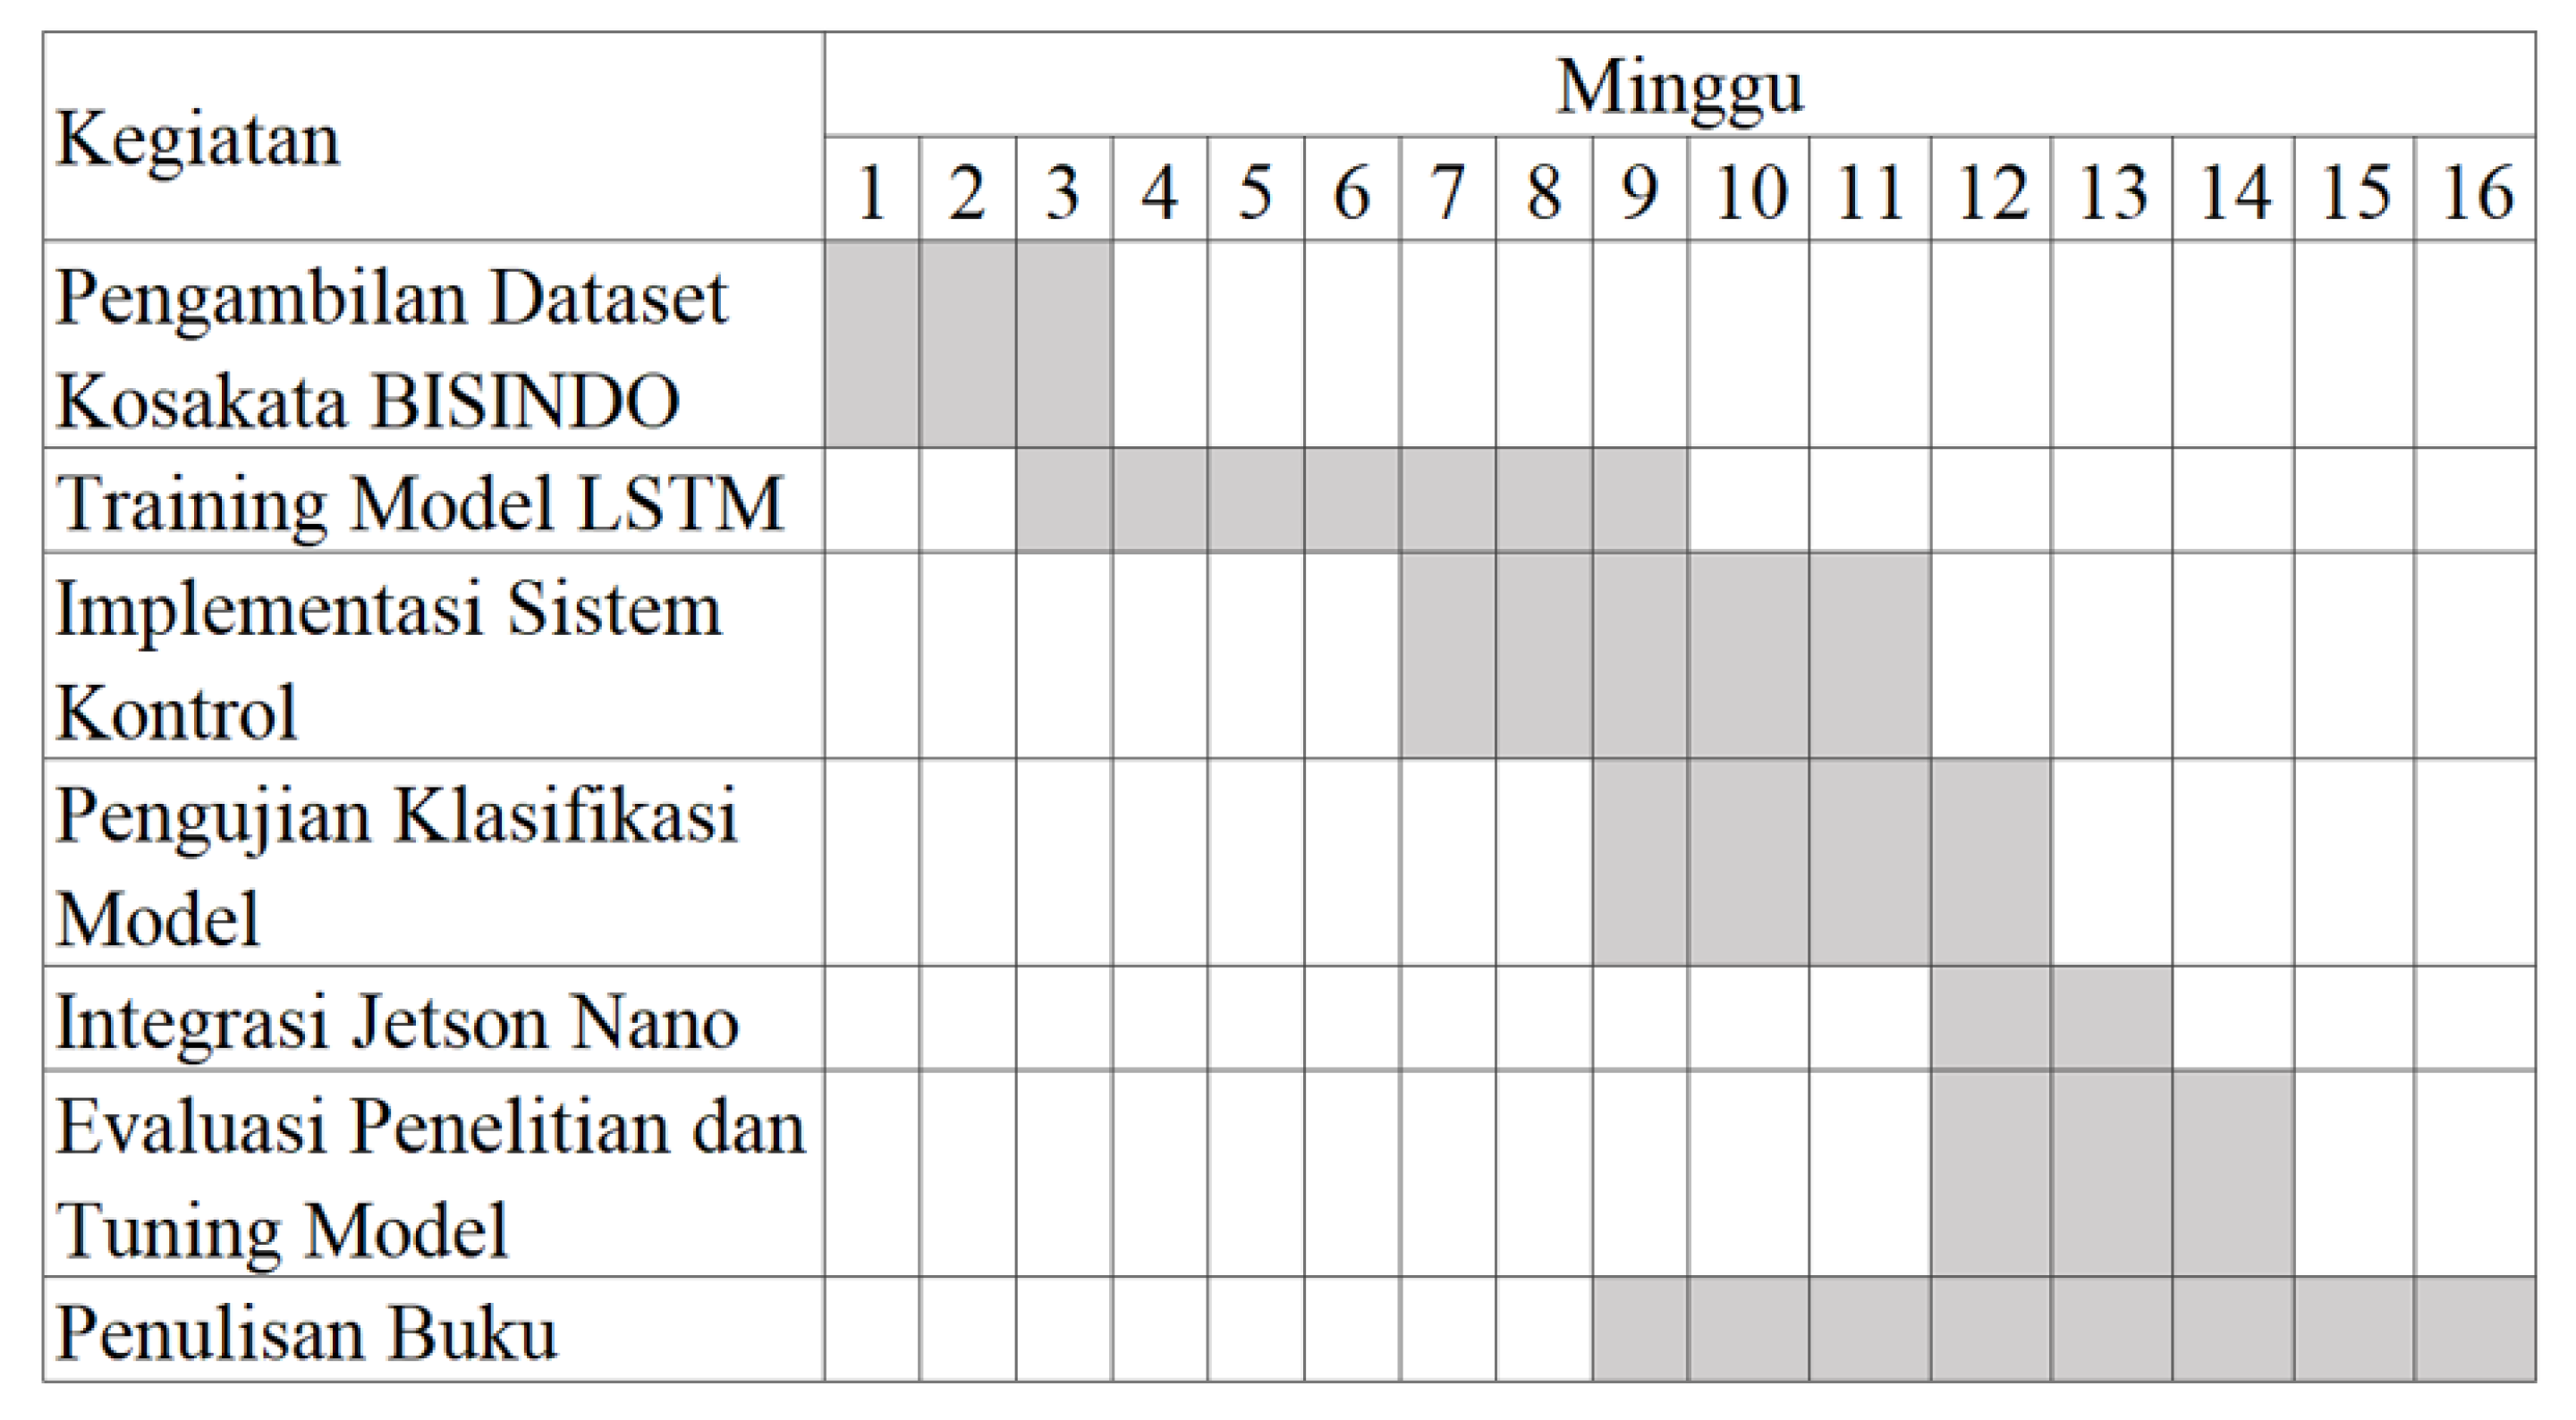
\includegraphics[scale=0.6]{gambar/bab3-timeline-kerja.png}
% \end{figure}

% \section{Deskripsi Sistem}
% \label{sec:deskripsisistem}

% Sistem akan dibuat dengan \lipsum[1-2]

% \section{Implementasi Alat
%   \label{sec:implementasi alat}}

% Alat diimplementasikan dengan \lipsum[1]

% % Contoh pembuatan potongan kode
% \begin{lstlisting}[
%   language=C++,
%   caption={Program halo dunia.},
%   label={lst:halodunia}
% ]
% #include <iostream>

% int main() {
%     std::cout << "Halo Dunia!";
%     return 0;
% }
% \end{lstlisting}

% \lipsum[2-3]

% % Contoh input potongan kode dari file
% \lstinputlisting[
%   language=Python,
%   caption={Program perhitungan bilangan prima.},
%   label={lst:bilanganprima}
% ]{program/bilangan-prima.py}

% \lipsum[4]

\cleardoublepage

% Bab 4 pengujian dan analisis
\chapter{PENGUJIAN DAN ANALISIS}
\label{chap:pengujiananalisis}

% Ubah bagian-bagian berikut dengan isi dari pengujian dan analisis

Pada bab ini akan dipaparkan skenario pengujian yang  dilakukan berdasarkan dari metodol\\ogi yang telah dibahas sebelumnya beserta dengan pembahasannya. Pengujian akan dilaksanakan untuk menjawab permasalahan yang diangkat sehingga dapat ditarik kesimpulan dari pelaksanaan tugas akhir ini.

\section{Skenario Pengujian}
\label{sec:skenariopengujian}

Pengujian ini akan dilakukan dengan menggunakan Intel NUC 11 Performance Kit yang telah terhubung ke internet untuk mengakses program melalui browser. Dibutuhkan juga tambahan koneksi dengan webcam eksternal sebagai media pengambilan data yang akan diproses pada program, serta keyboard, mouse, dan monitor untuk memudahkan dalam mengoperasikan program. Adapun pengujian ini akan mengikuti beberapa skenario - skenario pengujian yang ditentukan sebagai berikut:

\begin{enumerate}
  \item Skenario pengujian berdasarkan bentuk model
  \item Skenario pengujian berdasarkan kondisi pencahayaan yang berbeda, yaitu 35 lux, 80 lux, 125 lux. 
  \item Skenario pengujian berdasarkan jarak subjek yang berbeda, yaitu 180 cm, 240 cm, 300 cm.
  \item Skenario pengujian dengan menggunakan subjek yang berbeda selain penulis
  \item Skenario pengujian pembentukan kalimat dan koversi menjadi media suara
\end{enumerate}

\section{Pengujian Bentuk Model}
\label{sec:analisismodel}

Pengujian bentuk model penerjemah bahasa isyarat Indonesia (BISINDO) dilakukan dengan melakukan perubahan struktur dari \emph{layer} yang digunakan, baik dari segi pemilihan tipe \emph{layer}, fungsi \emph{activation}, serta jumlah unit aktivasi yang digunakan. Pengujian ini didasari dari struktur model yang telah dibahas pada sub bab \ref{sec:metodologipose}. Serangkaian model yang diuji akan dilihat bagaimana performa hasil dari \emph{training} model, melalui grafik \emph{accuracy} dan \emph{loss} yang dihasilkan. Digunakan \emph{confusion matrix} untuk mengamati bagaimana hasil dari pengujian model terhadap serangkaian data gerakan bahasa isyarat dengan membandingkan hasil prediksi model dengan data aktual yang ada untuk masing - masing kosakata atau \emph{class} yang ada. Berdasarkan \emph{confusion matrix} ini juga dapat dihasilkan matrix evaluasi berupa \emph{accuracy}, \emph{precision}, \emph{recall}, dan \emph{F1-score}. Setiap model yang diuji menggunakan partisi data \emph{training} dan validasi yang sama, yaitu dengan perbandingan 70:30. Hal ini menunjukkan bahwa dari keseluruhan data yang digunakan, akan terdapat 70\% data \emph{training} dan 30\% data validasi. Untuk setiap kosakata yang digunakan sesuai dengan yang telah dijelaskan pada sub bab \ref{sec:metodologidataset}. Keseluruhan model akan dilatih sebanyak 12 \emph{epoch}. Pengujian ini bertujuan untuk melihat bagaimana perubahan struktur dari \emph{layer} akan berpengaruh pada performa model penerjemah yang dihasilkan.

\subsection{Model Pertama}
\label{sec:analisismodel1}
Model pertama menggunakan 2 buah \emph{layer} LSTM. \emph{Layer} LSTM pertama menggunakan fungsi aktivasi \emph{relu} dan dengan unit aktivasi bernilai 128 dan \emph{layer} LSTM kedua menggunakan fungsi aktivasi \emph{relu} dan dengan unit aktivasi bernilai 64. Untuk setiap \emph{layer} LSTM akan diikuti dengan \emph{layer} Dropout bernilai 0.5 untuk mencegah nilai \emph{weight} yang terlalu tinggi. Setelah serangkaian \emph{layer} LSTM, diikuti dengan \emph{layer} Dense dengan fungsi aktivasi \emph{relu} dan dengan unit aktivasi bernilai 32. Struktur lengkap dari model ini dapat dilihat pada \ref{fig:model1-struktur}.

\begin{figure}[H]
  \centering

  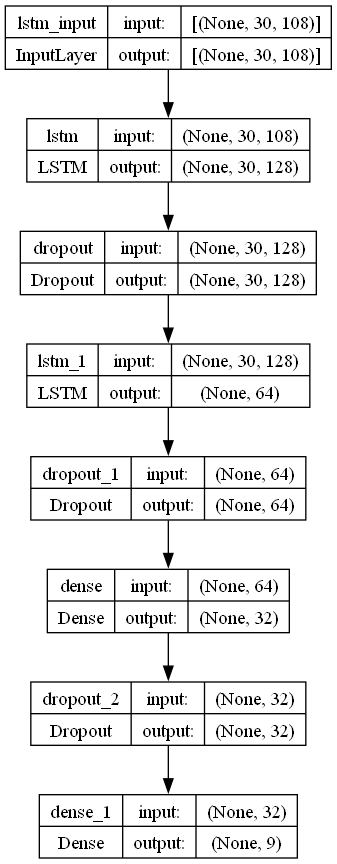
\includegraphics[scale=0.5]{gambar/bab4-uji-model-worst-model.png}

  \caption{Struktur model pertama}
  \label{fig:model1-struktur}
\end{figure}

Berdasarkan dari \emph{training} yang telah dilakukan didapatkan bahwa model menghasilkan akurasi validasi bernilai 0.89 dan akurasi \emph{training} bernilai 0.71. Data ini menunjukkan bahwa model memiliki akurasi yang cukup baik. Untuk nilai \emph{loss training} bernilai cukup tinggi, yaitu bernilai 2.81 dan \emph{loss} validasi bernilai 0.76 yang cukup rendanh jika dibandingkan dengan nilai \emph{loss training}. Nilai dari \emph{loss training} terlihat melonjak di \emph{epoch} terakhir, yaitu pada \emph{epoch} 12. Hal ini selaras dengan penurunan \emph{accuracy} model setelah \emph{epoch} 10. Grafik akurasi dan \emph{loss} dapat dilihat pada gambar \ref{fig:model1-train-acc} dan gambar \ref{fig:model1-train-loss}.

\begin{figure}[H]
  \centering

  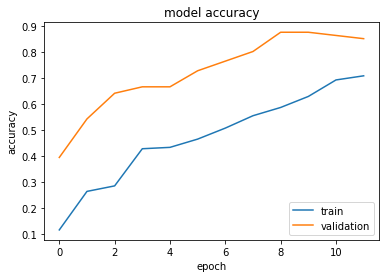
\includegraphics[scale=0.75]{gambar/bab4-uji-model-worst-acc.png}

  \caption{Hasil \emph{accuracy} model pertama}
  \label{fig:model1-train-acc}
\end{figure}

\begin{figure}[H]
  \centering

  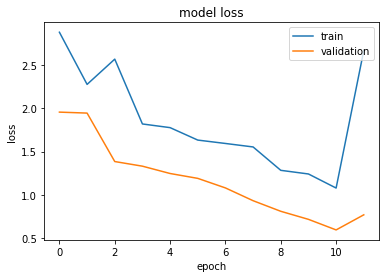
\includegraphics[scale=0.75]{gambar/bab4-uji-model-worst-loss.png}

  \caption{Hasil \emph{loss} model pertama}
  \label{fig:model1-train-loss}
\end{figure}

Kemudian berdasarkan model yang telah dihasilkan, dilakukan pengujian dengan dataset \emph{testing} yang menghasilkan \emph{confusion matrix}. Dapat dilihat pada gambar \ref{fig:model1-cf}, untuk kosakata "maaf", "tolong", "rumah", "delete", dan "translate" menghasilkan prediksi yang tepat untuk keseluruhan dataset \emph{testing} yang diujikan. Namun, kosakata "nama", "saya", "siapa", dan "standby" menghasilkan beberapa prediksi yang tidak sesuai dengan dataset \emph{testing}. Kosakata "nama" menghasilkan 6 prediksi tepat dan 4 prediksi yang kurang tepat (1 dataset \emph{testing} bernilai "siapa" dan 3 dataset \emph{testing} bernilai "rumah"). Kosakata "saya" menghasilkan 10 prediksi tepat dan 2 prediksi yang kurang tepat (dataset \emph{testing} bernilai "translate"). Kosakata "siapa" menghasilkan 3 prediksi tepat dan 5 prediksi yang kurang tepat (2 dataset \emph{testing} bernilai "tolong",  2 dataset \emph{testing} bernilai "saya", dan 1 dataset \emph{testing} bernilai "translate"). Kosakata "standby" menghasilkan 7 prediksi tepat dan 1 prediksi yang kurang tepat (dataset \emph{testing} bernilai "saya"). Adapun berdasarkan hasil \emph{confusion matrix} ini didapat matrix evaluasi berupa \emph{accuracy}, \emph{precision}, \emph{recall}, dan \emph{F1-score} yang dapat dilihat pada tabel \ref{tb:model1stat}. Rata - rata nilai \emph{accuracy} sebesar 0.85, rata - rata nilai \emph{precision} sebesar 0.85, rata - rata nilai \emph{recall} sebesar 0.85, dan rata - rata nilai \emph{F1-score} sebesar 0.83.

\begin{figure}[H]
  \centering

  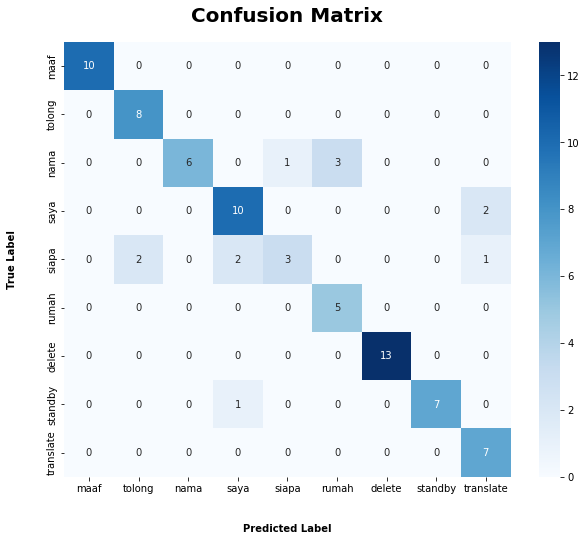
\includegraphics[scale=0.6]{gambar/bab4-uji-model-worst-cf.png}

  \caption{\emph{Confusion} model pertama}
  \label{fig:model1-cf}
\end{figure}

\begin{longtable}{|c|c|c|c|c|}
  \caption{Matrix Evaluasi Model 1}
  \label{tb:model1stat}                                   \\
  \hline
  \rowcolor[HTML]{C0C0C0}
  \textbf{Kosakata} & \textbf{\emph{Accuracy}} & \textbf{\emph{Precision}} & \textbf{\emph{Recall}} & \textbf{\emph{F1-Score}} \\
  \hline
  Maaf              & 1.00                     & 1.00                        & 1.00                   & 1.00                \\
  Tolong            & 1.00                     & 0.80                        & 1.00                   & 0.89                \\
  Nama              & 0.60                     & 1.00                        & 0.60                   & 0.75                \\
  Saya              & 0.83                     & 0.77                        & 0.83                   & 0.80                \\
  Siapa             & 0.37                     & 0.75                        & 0.38                   & 0.50                \\
  Rumah             & 1.00                     & 0.62                        & 1.00                   & 0.77                \\
  Delete            & 1.00                     & 1.00                        & 1.00                   & 1.00                \\
  Standby           & 0.87                     & 1.00                        & 0.88                   & 0.93                \\
  Translate         & 1.00                     & 0.70                        & 1.00                   & 0.82                \\
  \hline
\end{longtable}

\subsection{Model Kedua}
\label{sec:analisismodel2}

Model kedua diawali dengan \emph{layer} \textit{TimeDistributed} yang di dalamnya terdapat \emph{layer} \textit{Dense} dengan fungsi aktivasi '\textit{tanh}' dan unit aktivasi bernilai 128. Kemudian dilanjutkan dengan 1 buah \emph{layer} LSTM yang menggunakan fungsi aktivasi \emph{tanh} dan dengan unit aktivasi bernilai 64. \emph{Layer} LSTM akan diikuti dengan \emph{layer} Dropout bernilai 0.5 untuk mencegah nilai \emph{weight} yang terlalu tinggi. Setelah serangkaian \emph{layer} LSTM, diikuti dengan \emph{layer} Dense dengan fungsi aktivasi \emph{relu} dan dengan unit aktivasi bernilai 32. Struktur lengkap dari model ini dapat dilihat pada \ref{fig:model2-struktur}.

\begin{figure}[H]
  \centering

  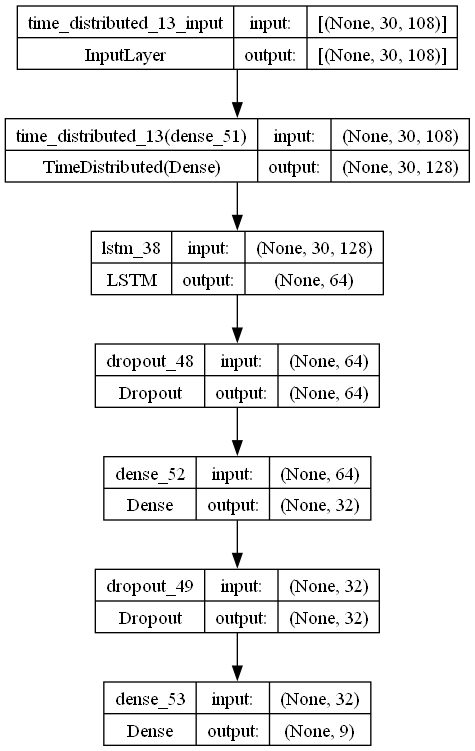
\includegraphics[scale=0.6]{gambar/bab4-uji-model-second-model.png}

  \caption{Struktur model kedua}
  \label{fig:model2-struktur}
\end{figure}

Berdasarkan dari \emph{training} yang telah dilakukan didapatkan bahwa model menghasilkan akurasi \emph{training} bernilai 0.96 dan akurasi validasi bernilai 0.93. Data ini menunjukkan bahwa model memiliki akurasi yang baik. Terdapat penurunan pada akurasi validasi pada \emph{epoch} terakhir, tetapi kebalikannya untuk akurasi \emph{training} mengalami kenaikan melebihi akurasi validasi. Untuk nilai \emph{loss training} bernilai 0.32 dan \emph{loss} validasi bernilai 0.25 yang cukup rendah jika dibandingkan dengan nilai \emph{loss training}. Data ini menunjukkan bahwa model memiliki \emph{error} prediksi yang kecil. Grafik akurasi dan \emph{loss} dapat dilihat pada gambar \ref{fig:model2-train-acc} dan gambar \ref{fig:model2-train-loss}.

\begin{figure}[H]
  \centering

  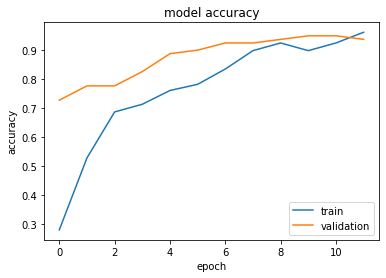
\includegraphics[scale=0.75]{gambar/bab4-uji-model-second-acc.png}

  \caption{Hasil \emph{accuracy} model kedua}
  \label{fig:model2-train-acc}
\end{figure}

\begin{figure}[H]
  \centering

  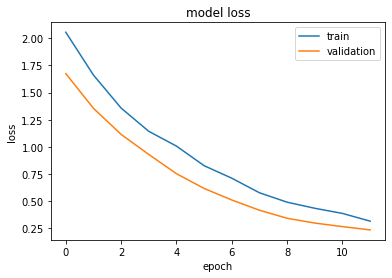
\includegraphics[scale=0.75]{gambar/bab4-uji-model-second-loss.png}

  \caption{Hasil \emph{loss} model kedua}
  \label{fig:model2-train-loss}
\end{figure}


Kemudian berdasarkan model yang telah dihasilkan, dilakukan pengujian dengan dataset \emph{testing} yang menghasilkan \emph{confusion matrix}. Dapat dilihat pada gambar \ref{fig:model2-cf}, untuk kosakata "tolong", "nama", "rumah", "delete", dan "translate" menghasilkan prediksi yang tepat untuk keseluruhan dataset \emph{testing} yang diujikan. Namun, kosakata "saya", "siapa", dan "standby" menghasilkan beberapa prediksi yang tidak sesuai dengan dataset \emph{testing}. Kosakata "maaf" menghasilkan 10 prediksi tepat dan 1 prediksi yang kurang tepat (dataset \emph{testing} bernilai "standb\\y"). Kosakata "saya" menghasilkan 11 prediksi tepat dan 2 prediksi yang kurang tepat (dataset \emph{testing} bernilai "siapa"). Kosakata "siapa" menghasilkan 5 prediksi tepat dan 1 prediksi yang kurang tepat (dataset \emph{testing} bernilai "saya"). Kosakata "standby" menghasilkan 7 prediksi tepat dan 1 prediksi yang kurang tepat (dataset \emph{testing} bernilai "siapa"). Dapat dilihat bahwa terdapat peningkatan performa dari model pertama dengan model kedua. Kosakata yang berhasil diprediksi sesuai dengan dataset \emph{testing} yang digunakan lebih banyak dibandingkan dengan model sebelumnya, yaitu 5 kosakata. Peningkatan ini disebabkan karena perubahan struktur dari model dengan adanya penggunaan \emph{layer Time Distributed} yang di dalamnya diisi dengan \emph{layer} Dense di lapisan awal model. Pengurangan pengunaan 1 \emph{layer} LSTM dapat dengan menggunakan fungsi aktivasi \emph{tanh}. Adapun berdasarkan \emph{confusion matrix} ini didapat matrix evaluasi berupa \emph{accuracy}, \emph{precision}, \emph{recall}, dan \emph{F1-score} yang dapat dilihat pada tabel \ref{tb:model2stat}. Rata - rata nilai \emph{accuracy} sebesar 0.93, nilai \emph{precision} sebesar 0.95, rata - rata nilai \emph{recall} sebesar 0.94, dan rata - rata nilai \emph{F1-score} sebesar 0.94. Dapat dilihat berdasarkan matrix evaluasi ini, terdapat peningkatan performa pada model kedua jika dibandingkan dengan model pertama. 

\begin{figure}[H]
  \centering

  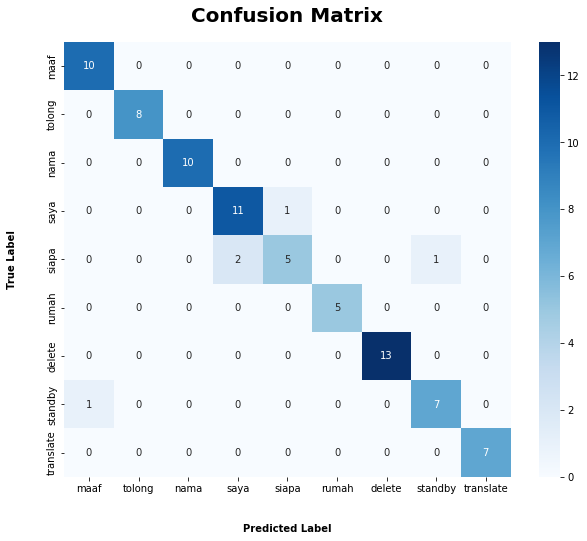
\includegraphics[scale=0.6]{gambar/bab4-uji-model-second-cf.png}

  \caption{\emph{Confusion} model kedua}
  \label{fig:model2-cf}
\end{figure}

\begin{longtable}{|c|c|c|c|c|}
  \caption{Matrix Evaluasi Model 2}
  \label{tb:model2stat}                                   \\
  \hline
  \rowcolor[HTML]{C0C0C0}
  \textbf{Kosakata} & \textbf{\emph{Accuracy}} & \textbf{\emph{Precision}} & \textbf{\emph{Recall}} & \textbf{\emph{F1-Score}} \\
  \hline
  Maaf              & 1.00                        & 0.91                        & 1.00                   & 0.95                \\
  Tolong            & 1.00                        & 1.00                        & 1.00                   & 1.00                \\
  Nama              & 1.00                        & 1.00                        & 1.00                   & 1.00                \\
  Saya              & 0.91                        & 0.85                        & 0.92                   & 0.88                \\
  Siapa             & 0.62                        & 0.93                        & 0.62                   & 0.71                \\
  Rumah             & 1.00                        & 1.00                        & 1.00                   & 1.00                \\
  Delete            & 1.00                        & 1.00                        & 1.00                   & 1.00                \\
  Standby           & 0.87                        & 0.88                        & 0.88                   & 0.88                \\
  Translate         & 1.00                        & 1.00                        & 1.00                   & 1.00                \\
  \hline
\end{longtable}

\subsection{Model Ketiga}
\label{sec:analisismodel3}

Model ketiga merupakan gabungan dari struktur antara model 1 dan model 2. Model ini diawali dengan layer pertama berupa \emph{layer} \textit{TimeDistributed} yang di dalamnya terdapat \emph{layer} \textit{Dense} dengan fungsi aktivasi '\textit{tanh}' dan unit aktivasi bernilai 128. Selanjutnya diikuti dengan 2 buah \emph{layer} LSTM. \emph{Layer} LSTM pertama menggunakan fungsi aktivasi \emph{tanh} dengan unit aktivasi bernilai 128 dan \emph{Layer} LSTM kedua menggunakan fungsi aktivasi \emph{tanh} dengan unit aktivasi bernilai 64. Kedua \emph{layer} LSTM ini diikuti dengan \emph{layer} Dropout bernilai 0.5 untuk mencegah nilai \emph{weight} yang terlalu tinggi. Dilanjutkan dengan \emph{layer} Dense dengan fungsi aktivasi \emph{relu} dan unit aktivasi bernilai 32. Struktur lengkap dari model ini dapat dilihat pada gambar \ref{fig:model3-struktur}

\begin{figure}[H]
  \centering

  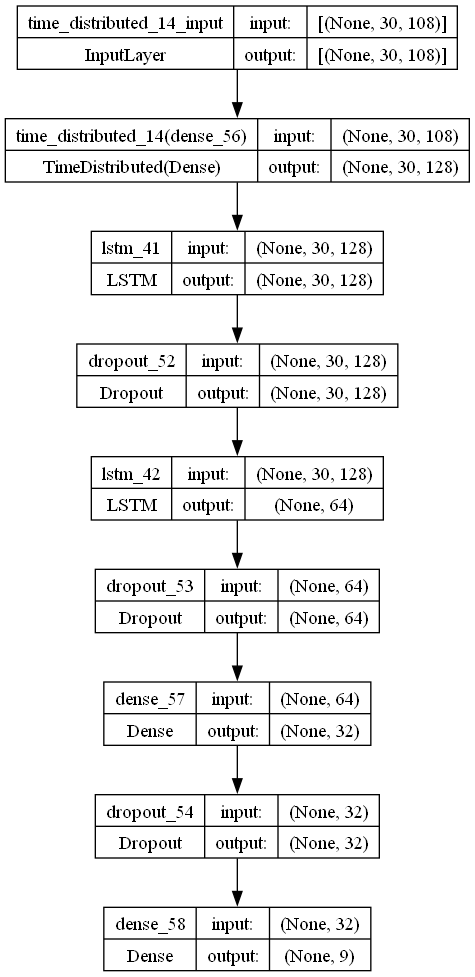
\includegraphics[scale=0.5]{gambar/bab4-uji-model-best-model.png}

  \caption{Struktur model ketiga}
  \label{fig:model3-struktur}
\end{figure}

Berdasarkan dari \emph{training} yang telah dilakukan didapatkan bahwa model menghasilkan akurasi \emph{training} bernilai 0.94 dan akurasi validasi bernilai 1.00. Data ini menunjukkan bahwa model memiliki akurasi yang sangat baik. Untuk nilai \emph{loss training} bernilai 0.3 dan \emph{loss} validasi bernilai 0.16 yang rendah jika dibandingkan dengan nilai \emph{loss training}. Data ini menunjukkan bahwa model memiliki \emph{error} prediksi yang kecil. Hasil dari \emph{training} model ini menunjukkan bahwa model telah dapat mempelajari dataset dengan baik. Ketika dilakukan pengujian dengan menggunakan data validasi, dapat dilihat bahwa model memiliki akurasi yang lebih tinggi dan tingkat \emph{loss} yang lebih rendah dibandingkan dengan pengujian yang menggunakan data \emph{training} itu sendiri. Grafik akurasi dan \emph{loss} dapat dilihat pada gambar \ref{fig:model3-train-acc} dan gambar \ref{fig:model3-train-loss}.

\begin{figure}[H]
  \centering

  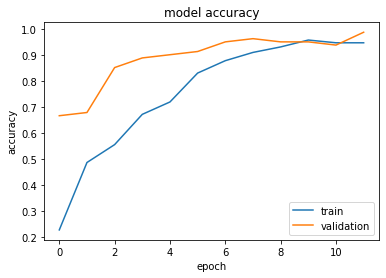
\includegraphics[scale=0.75]{gambar/bab4-uji-model-best-acc.png}

  \caption{Hasil \emph{accuracy} model ketiga}
  \label{fig:model3-train-acc}
\end{figure}

\begin{figure}[H]
  \centering

  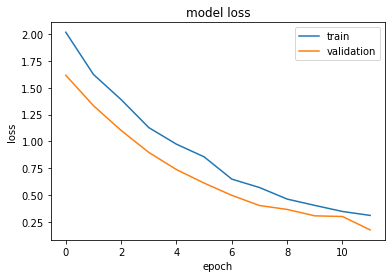
\includegraphics[scale=0.75]{gambar/bab4-uji-model-best-loss.png}

  \caption{Hasil \emph{loss} model ketiga}
  \label{fig:model3-train-loss}
\end{figure}


Kemudian berdasarkan model yang telah dihasilkan, dilakukan pengujian dengan dataset \emph{testing} yang menghasilkan \emph{confusion matrix}. Dapat dilihat pada gambar \ref{fig:model3-cf}, untuk kosakata "maaf", "tolong", "nama", "saya",  menghasilkan prediksi yang tepat untuk keseluruhan dataset \emph{testing} yang diujikan. Namun, pada kosakata "siapa" menghasilkan beberapa prediksi yang tidak sesuai dengan dataset \emph{testing}. Kosakata "siapa" menghasilkan 7 prediksi tepat dan 1 prediksi yang kurang tepat (dataset \emph{testing} bernilai "saya"). Dapat dilihat bahwa terdapat peningkatan performa dari model ketiga dibandingkan dengan model pertama dan kedua. Peningkatan ini disebabkan karena perubahan struktur dari model dengan penggunaan \emph{layer Time Distributed} yang didalamnya diisi dengan \emph{layer} Dense di lapisan awal model. Kemudian dilanjutkan dengan 2 buah \emph{layer} LSTM yang menggunakan fungsi aktivasi \emph{tanh} Adapun berdasarkan \emph{confusion matrix} ini didapat matrix evaluasi berupa \emph{accuracy}, \emph{precision}, \emph{recall}, dan \emph{F1-score} yang dapat dilihat pada tabel \ref{tb:model3stat}. Rata - rata nilai \emph{accuracy} sebesar 0.99, rata - rata nilai \emph{precision} sebesar 0.99 rata - rata nilai \emph{recall} sebesar 0.98, dan rata - rata nilai \emph{F1-score} sebesar 0.99. Dapat dilihat berdasarkan matrix evaluasi ini, terdapat peningkatan performa pada model ketiga jika dibandingkan dengan model pertama dan kedua.

\begin{figure}[H]
  \centering

  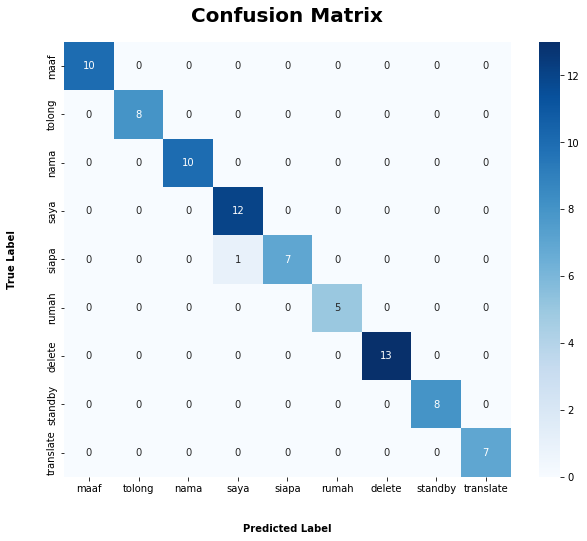
\includegraphics[scale=0.6]{gambar/bab4-uji-model-best-cf.png}

  \caption{\emph{Confusion} model pertama}
  \label{fig:model3-cf}
\end{figure}

\newpage
\begin{longtable}{|c|c|c|c|c|c|}
  \caption{Matrix Evaluasi Model 3}
  \label{tb:model3stat}                                   \\
  \hline
  \rowcolor[HTML]{C0C0C0}
  \textbf{Kosakata} & \textbf{\emph{Accuracy}} & \textbf{\emph{Precision}} & \textbf{\emph{Recall}} & \textbf{\emph{F1-Score}} \\
  \hline
  Maaf              & 1.00                       & 1.00                        & 1.00                   & 1.00                \\
  Tolong            & 1.00                       & 1.00                        & 1.00                   & 1.00                \\
  Nama              & 1.00                       & 1.00                        & 1.00                   & 1.00                \\
  Saya              & 1.00                       & 0.92                        & 1.00                   & 0.96                \\
  Siapa             & 0.87                       & 1.00                        & 0.82                   & 0.93                \\
  Rumah             & 1.00                       & 1.00                        & 1.00                   & 1.00                \\
  Delete            & 1.00                       & 1.00                        & 1.00                   & 1.00                \\
  Standby           & 1.00                       & 1.00                        & 1.00                   & 1.00                \\
  Translate         & 1.00                       & 1.00                        & 1.00                   & 1.00                \\
  \hline
\end{longtable}

\subsection{Rangkuman Pengujian Bentuk Model}
\label{sec:analisismodelseluruh}

\begin{longtable}{|c|c|c|c|c|}
  \caption{Rangkuman Pengujian Bentuk Model}
  \label{tb:evaluasiModel}                                   \\
  \hline
  \rowcolor[HTML]{C0C0C0}
  \textbf{Model} & \emph{\textbf{Avg. Accuracy}} & \emph{\textbf{Avg. Precision}} & \emph{\textbf{Avg. Recall}} & \emph{\textbf{Avg. F1-Score}} \\
  \hline
  Model 1 & 0.85 & 0.85 & 0.85 & 0.83 \\
  Model 2 & 0.93 & 0.95 & 0.94 & 0.94 \\
  Model 3 & 0.99 & 0.99 & 0.98 & 0.99 \\
  \hline
\end{longtable}

Secara keseluruhan, berdasarkan tabel \ref{tb:evaluasiModel} bahwa seiring denagn peningkatan kompleksitas dari suatu model selaras dengan peningkatan performa dari model itu sendiri. Hal ini dapat ditunjukkan dengan peningkatan akurasi dari model 1, yaitu 0.85 atau 85\% menjadi pada model 3, yaitu 0.99 atau 99\%. Nilai \emph{average precision}, {average recall},dan \emph{average F1-Score} juga meningkat seiring dengan peningkatan stuktur dari model. Penggunaan \emph{layer TimeDistributed} dan diikuti 2 \emph{layer} LSTM menghasilkan model dengan performa terbaik.

\section{Pengujian Kondisi Cahaya}
\label{sec:analisiscahaya}

Pada pengujian kondisi cahaya ini dilakukan untuk memahami bagaimana performa model dalam kondisi intensitas cahaya  yang berbeda - beda. Adapun intensitas cahaya yang akan digunakan pada pengujian ini adalah 35 lux (kondisi ruangan gelap), 80 lux (kondisi ruangan remang - remang), dan 125 lux (kondisi ruangan terang). Variasi intensitas cahaya ini dipilih karena merupakan intensitas cahaya yang umum ditemukan pada ruangan tertutup. Kondisi ruangan dengan intensitas cahaya masing - masing dapat dilihat pada tabel \ref{tb:kondisicahaya}. Pengambilan nilai intensitas cahaya ini dilakukan dengan menggunakan \emph{lux meter} yang telah dikalibrasi untuk memastikan ketelitian hasil pengukuran.

Model penerjemah bahasa Indonesia (BISINDO) yang akan digunakan pada pengujian ini adalah model pada bagian \ref{sec:analisismodel3} karena merupakan model yang menghasilkan klasifikasi yang terbaik jika dibandingkan dengan model lainnya. Untuk setiap intensitas cahaya akan dilakukan pengujian sebanyak tiga kali dengan jarak terhadap kamera sebesar 300 cm. Pada setiap pengujian akan dicari hasil klasifikasi model, waktu yang dibutuhkan model untuk menghasilkan klasifikasi bahasa isyarat berdasarkan data koordinat yang diberikan(\emph{processing time}), dan waktu total yang dibutuhkan dalam menghasilkan klasifikasi bahasa isyarat (\emph{complete time}).  

\newpage
\begin{longtable}{|c|c|}
  \caption{Variasi Kondisi Cahaya}
  \label{tb:kondisicahaya}                                   \\
  \hline
  \rowcolor[HTML]{C0C0C0}
  \textbf{Intensitas Cahaya} & \textbf{Gambar Kondisi}  \\
  \hline
  35 lux            &  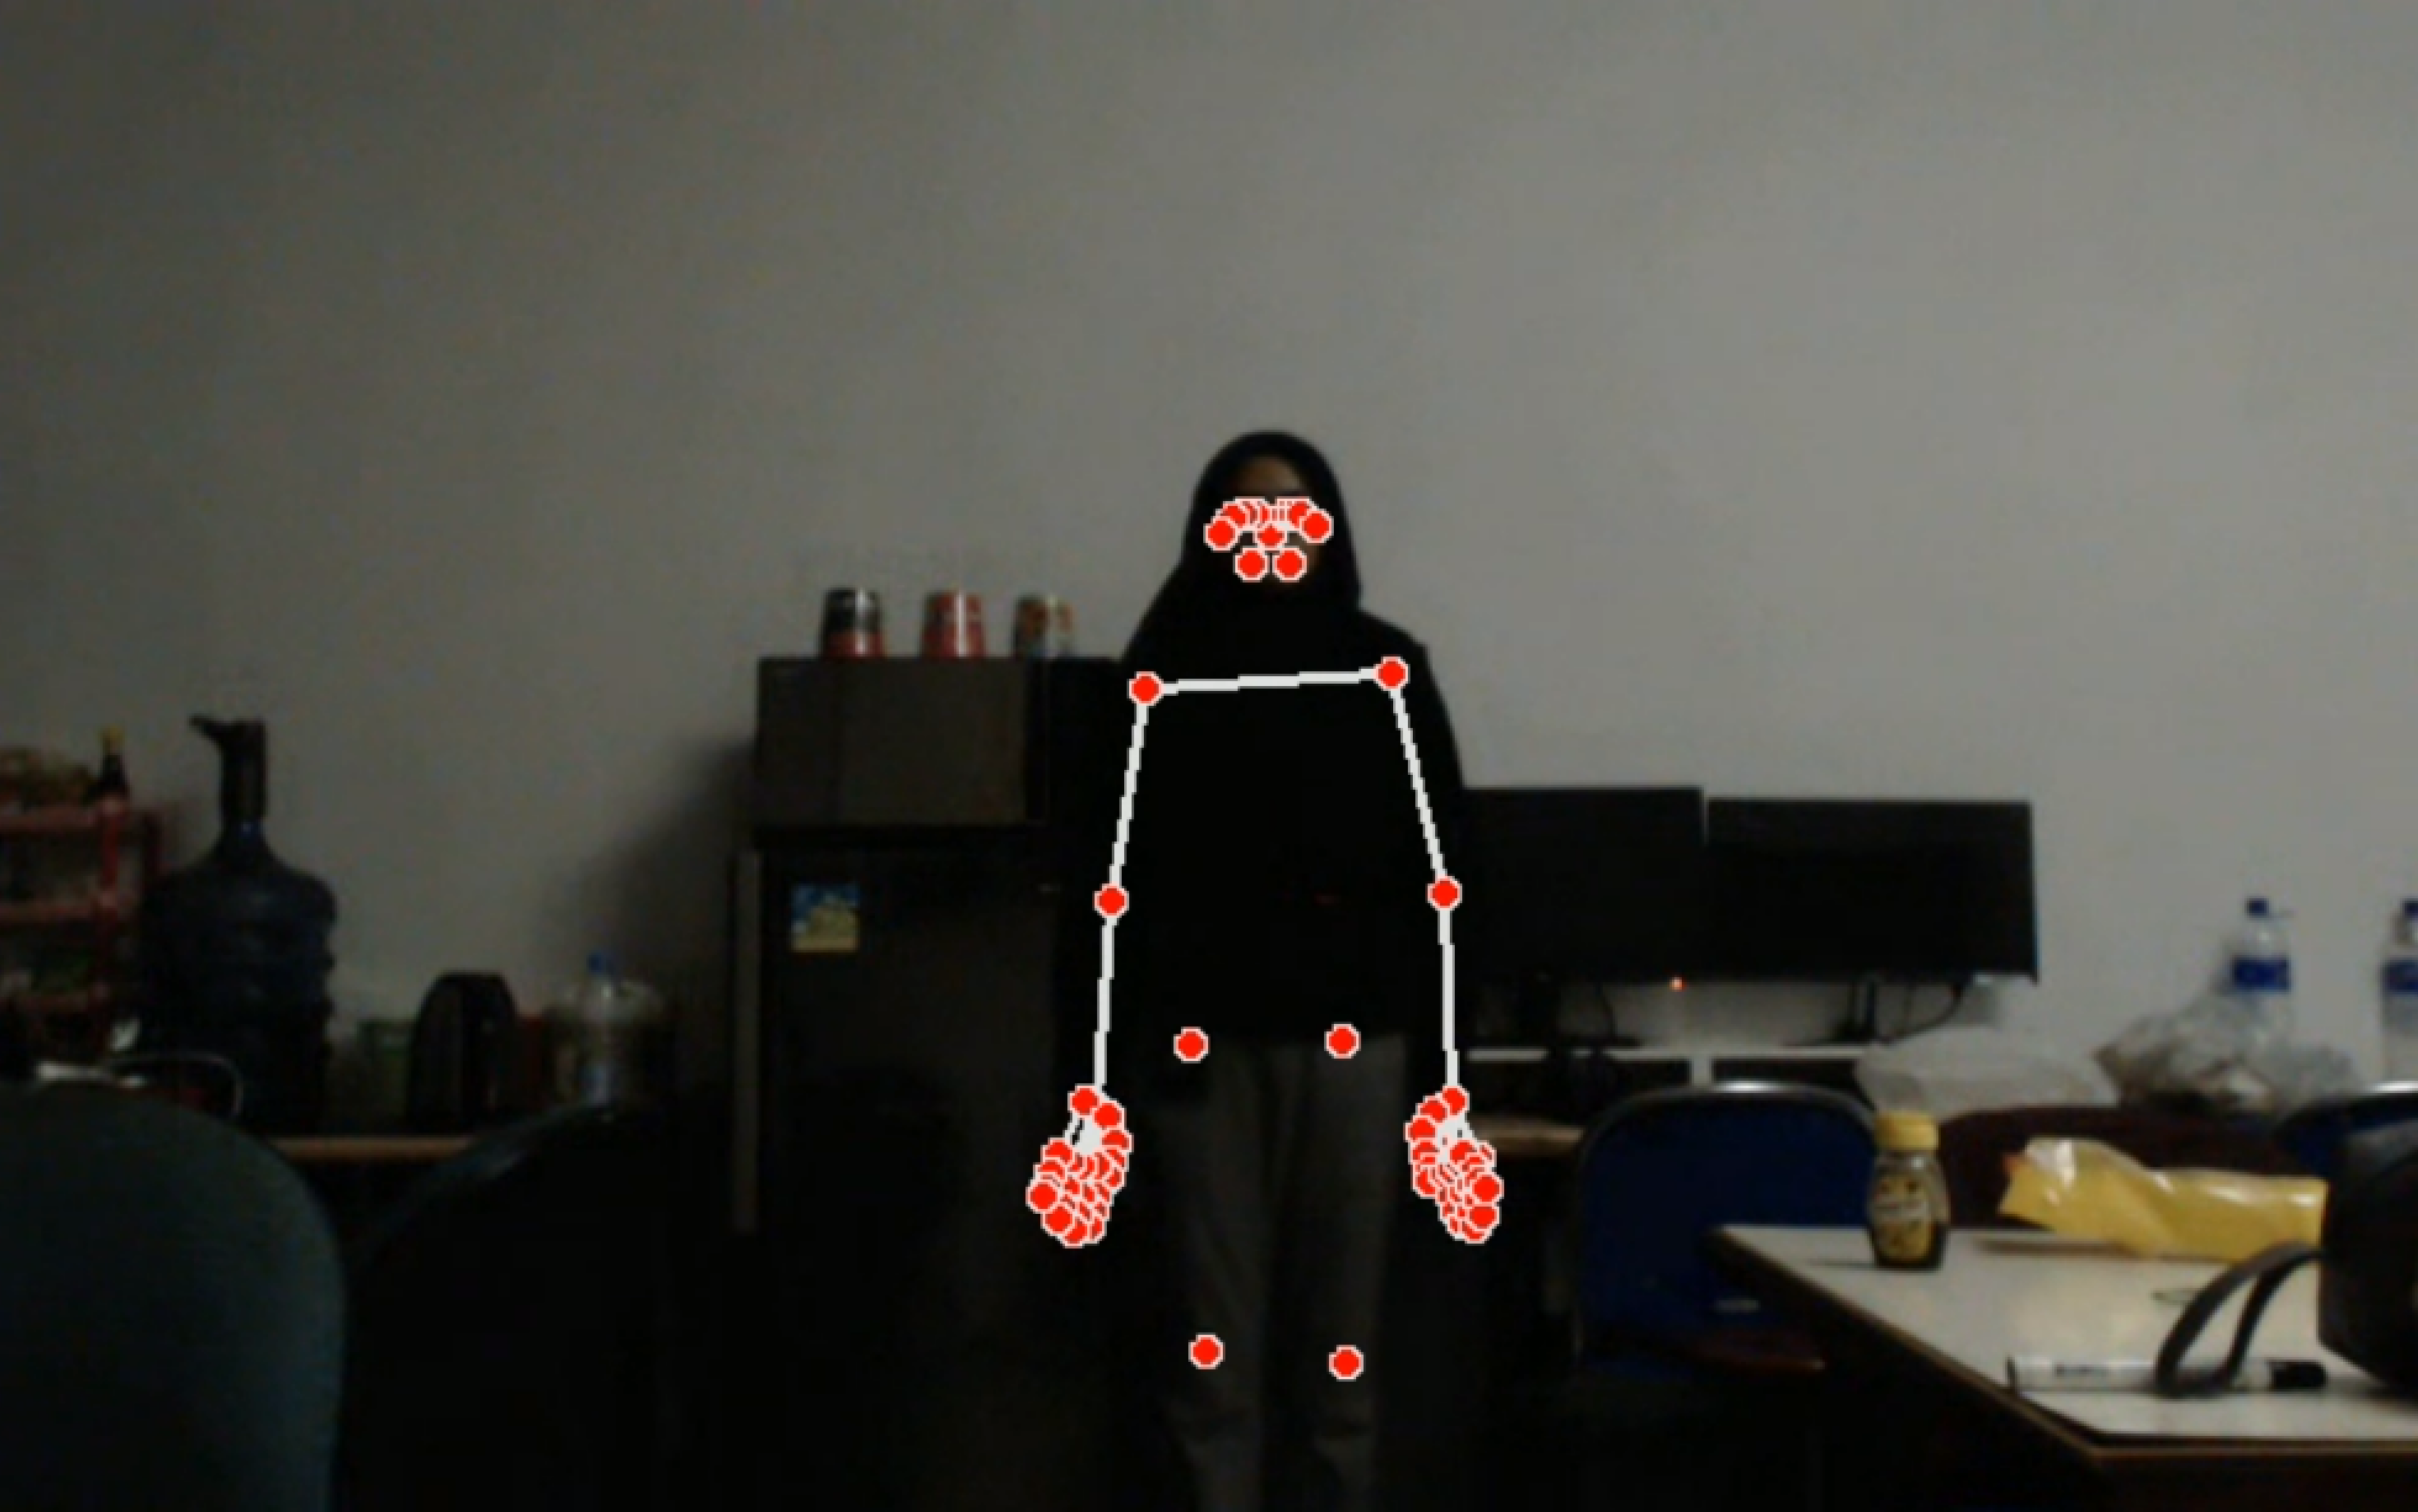
\includegraphics[scale=0.3]{gambar/bab4-gelap.png}                \\
  \hline
  80 lux            & 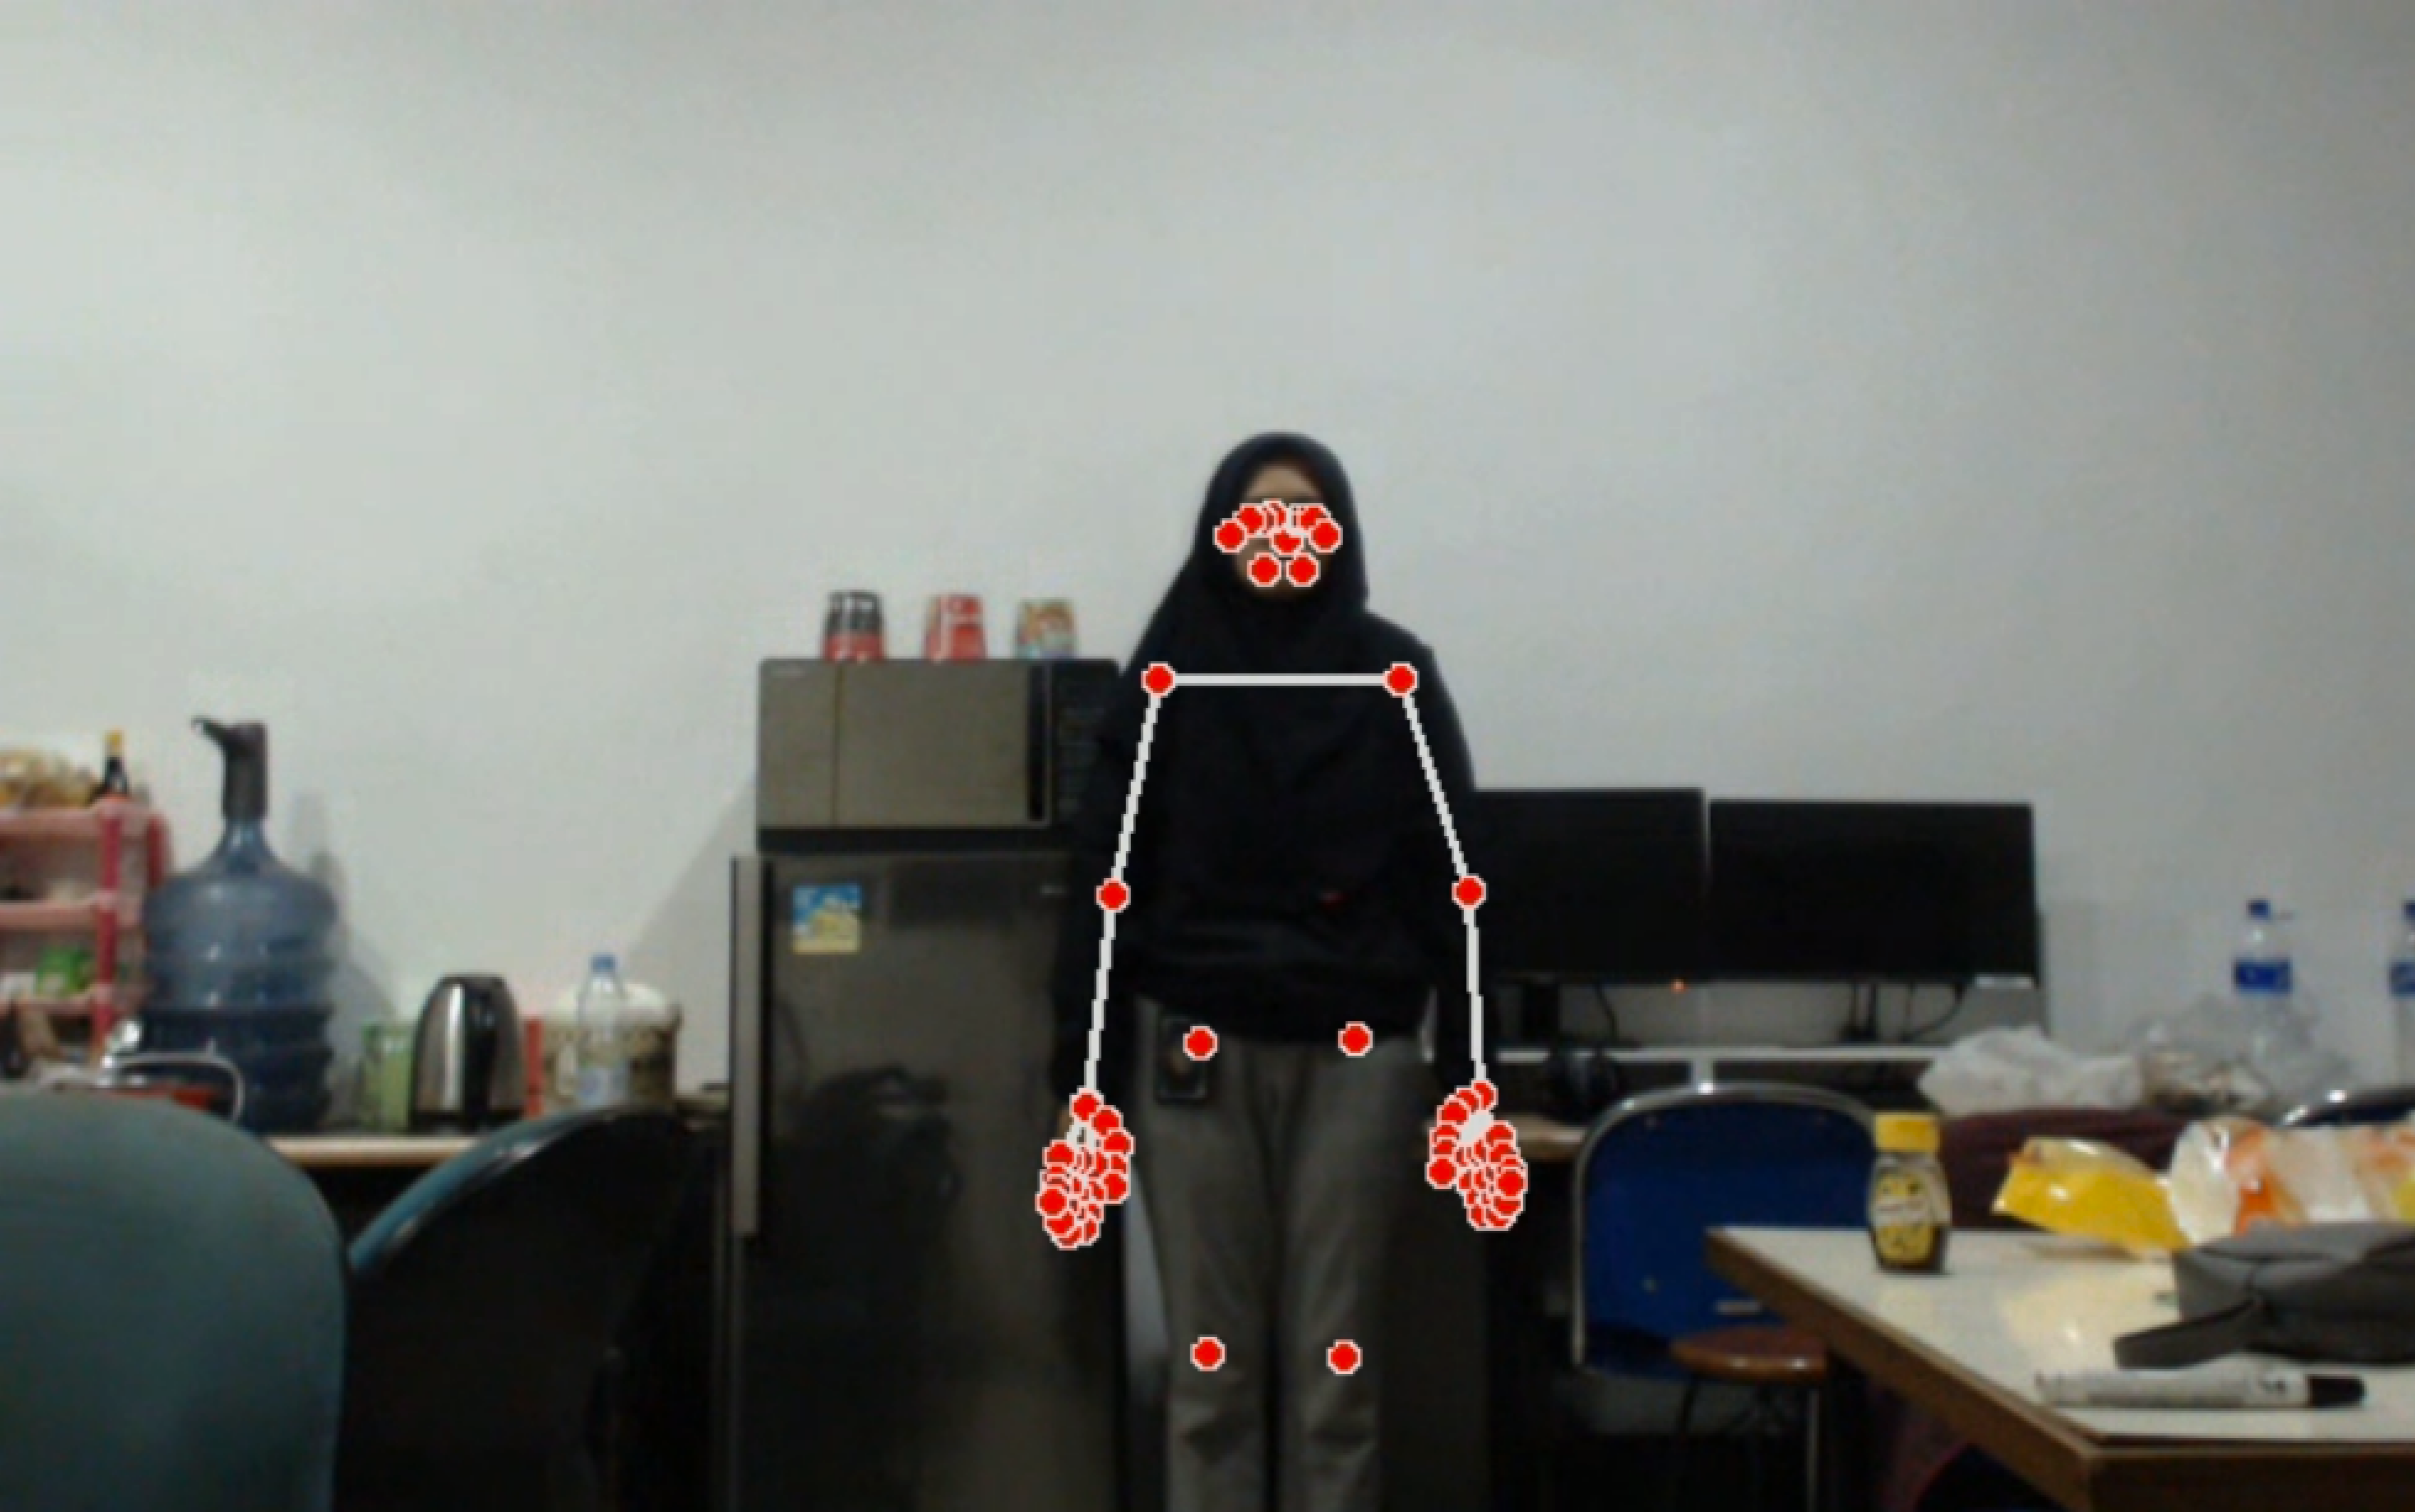
\includegraphics[scale=0.3]{gambar/bab4-remang.png}                 \\
  \hline
  125 lux            & 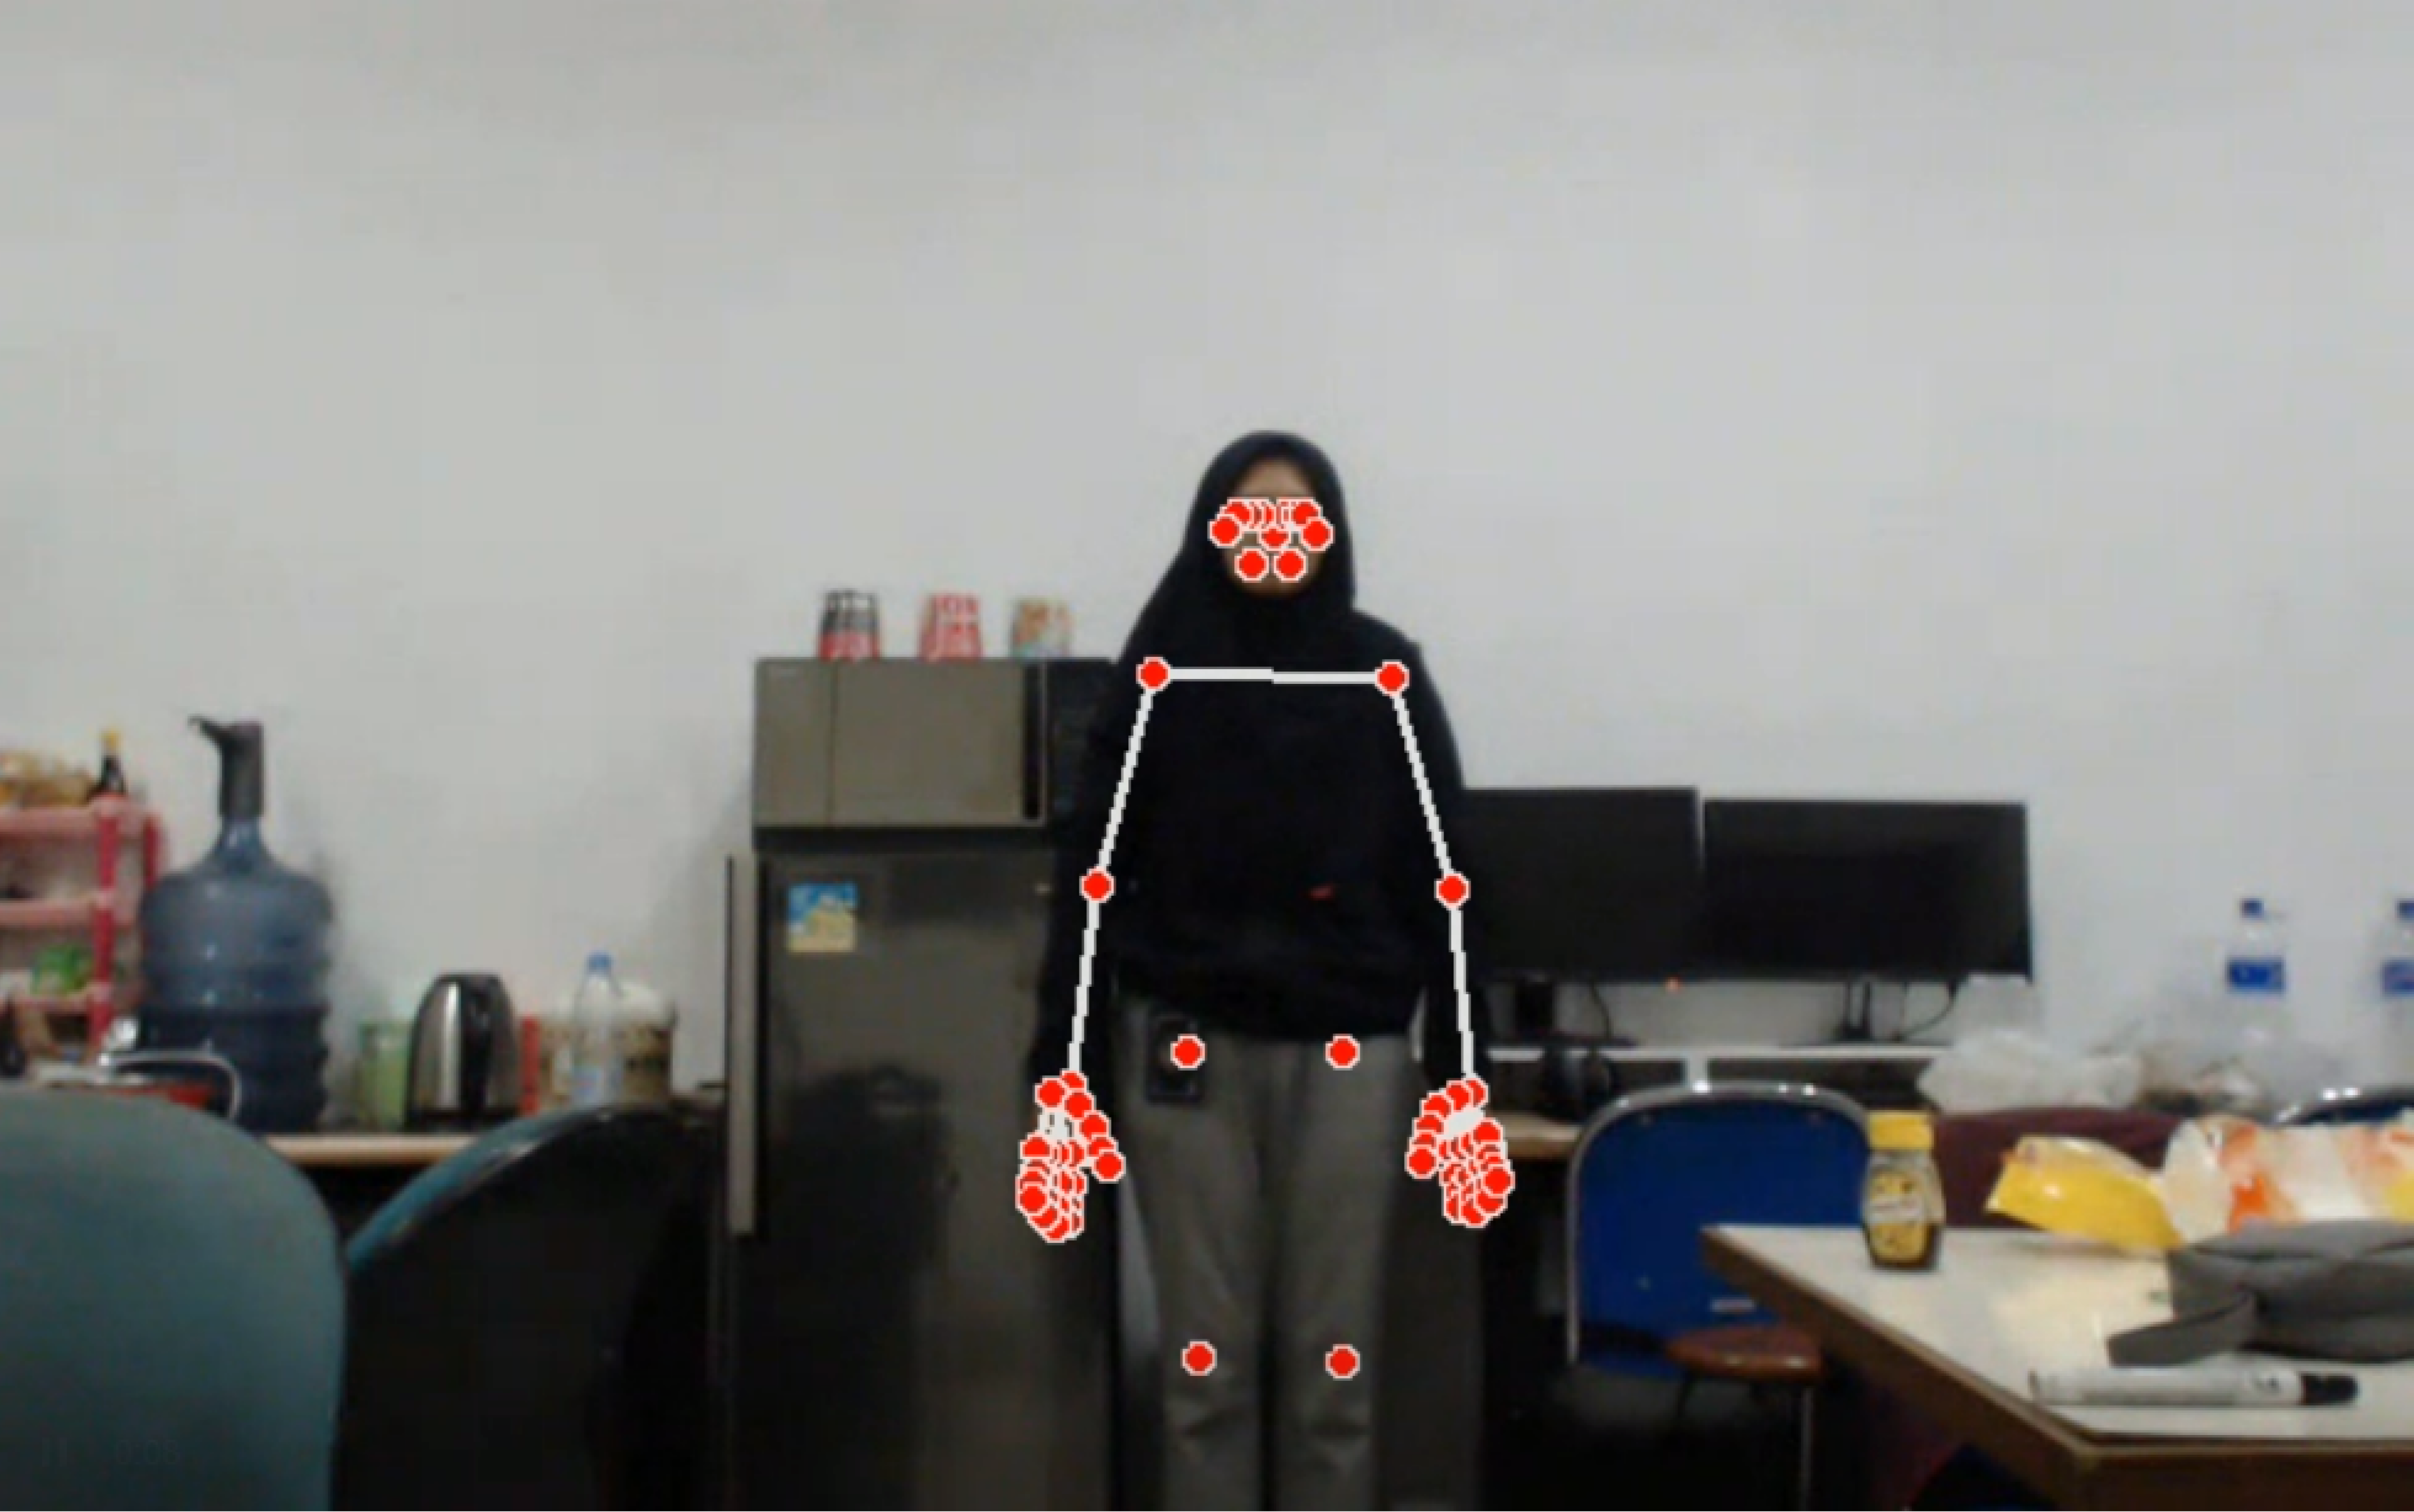
\includegraphics[scale=0.3]{gambar/bab4-terang.png}                 \\
  \hline
\end{longtable}

\newpage
\subsection{Pengujian Model di Kondisi Cahaya 35 lux}
\label{sec:analisiscahaya1}

\begin{longtable}{|c|c|c|c|}
  \caption{Pengujian Pertama Model di Kondisi Cahaya 35 lux}
  \label{tb:prediksigelap1}                                   \\
  \hline
  \rowcolor[HTML]{C0C0C0}
  \textbf{Kosakata} & \textbf{Klasifikasi Model} & \textbf{\emph{Processing Time}} & \textbf{\emph{Complete Time}}\\
  \hline
  Maaf              & Maaf                          & 0.09208822250366211 detik                           & 2.8735828399658203 detik                                  \\
  Tolong            & Tolong                        & 0.09197822450361212 detik                           & 2.9096102714538574 detik                                  \\
  Nama              & Nama                          & 0.08932256698608398 detik                           & 3.3274698257446294 detik                                  \\
  Saya              & Saya                          & 0.09866833686828613 detik                           & 2.8822731971740723 detik                                  \\
  Siapa             & Siapa                         & 0.08973073959350586 detik                           & 2.8529834747314453 detik                                  \\
  Rumah             & \textcolor{red}{Delete}       & 0.09612202644348145 detik                           & 2.8643417358398438 detik                                  \\
  Delete            & Delete                        & 0.09255480766296387 detik                           & 2.824845314025879 detik                                 \\
  Standby           & Standby                       & 0.09247112274169922 detik                           & 2.8762435913085938 detik                                  \\
  Translate         & Translate                     & 0.09525346755981445 detik                           & 2.9262471199035645 detik                                  \\
  \hline
\end{longtable}

\begin{longtable}{|c|c|c|c|}
  \caption{Pengujian Kedua Model di Kondisi Cahaya 35 lux}
  \label{tb:prediksigelap2}                                   \\
  \hline
  \rowcolor[HTML]{C0C0C0}
  \textbf{Kosakata} & \textbf{Klasifikasi Model} & \textbf{\emph{Processing Time}} & \textbf{\emph{Complete Time}} \\
  \hline
  Maaf              & Maaf                            & 0.10043215751647949 detik                           & 3.328549861907959 detik                                 \\
  Tolong            & Tolong                          & 0.0972287654876709 detik                            & 3.3190798759460445 detik                                  \\
  Nama              & \textcolor{red}{Standby}        & 0.08973073959350586 detik                           & 2.914302349090576 detik                                 \\
  Saya              & Saya                            & 0.1007227897644043 detik                            & 2.789583206176758 detik                                 \\
  Siapa              & Siapa                          & 0.08973073959350586 detik                           & 3.4017491340637203 detik                                  \\
  Rumah             & Rumah                           & 0.10046267509460449 detik                           & 2.94283390045166 detik                                \\
  Delete            & Delete                          & 0.09255480766296387 detik                           & 2.9163265228271484 detik                                  \\
  Standby           & Standby                         & 0.09181642532348633 detik                           & 2.8268051147460938 detik                                  \\
  Translate         & Translate                       & 0.08920478820800781 detik                           & 3.3912491798400874 detik                                  \\
  \hline
\end{longtable}

\begin{longtable}{|c|c|c|c|}
  \caption{Pengujian Ketiga Model di Kondisi Cahaya 35 lux}
  \label{tb:prediksigelap3}                                   \\
  \hline
  \rowcolor[HTML]{C0C0C0}
  \textbf{Kosakata} & \textbf{Klasifikasi Model} & \textbf{\emph{Processing Time}} & \textbf{\emph{Complete Time}}\\
  \hline
  Maaf              & Maaf                          & 0.09208822250366211 detik                           & 2.9158973693847656 detik                                  \\
  Tolong            & Tolong                        & 0.0972287654876709 detik                            & 3.0014920234680176 detik                                  \\
  Nama              & Nama                          & 0.09724950790405273 detik                           & 2.8235292434692383 detik                                  \\
  Saya              & Saya                          & 0.08916234970092773 detik                           & 2.9606938362121578 detik                                  \\
  Siapa             & Siapa                         & 0.08973073959350586 detik                           & 2.8408455848693848 detik                                  \\
  Rumah             & \textcolor{red}{Delete}       & 0.10066267509460449 detik                           & 3.36672306060791 detik                                \\
  Delete            & Delete                        & 0.09255480766296387 detik                           & 3.4308242797851562 detik                                  \\
  Standby           & Standby                       & 0.09866833686828613 detik                           & 3.3450722694396973 detik                                  \\
  Translate         & Translate                     & 0.08920478820800781 detik                           & 2.830524444580078 detik                                 \\
  \hline
\end{longtable}

Berdasarkan tiga pengujian yang telah dilakukan, didapatkan bahwa hampir keseluruhan klasifikasi model yang sesuai dengan \emph{class} kosakata. Namun, terdapat beberapa kesalahan model dalam melakukan klasifikasi. Dapat dilihat pada tabel \ref{tb:prediksigelap1} untuk kosakata "Rumah" diklasifikasikan sebagai "Delete". Kesalahan ini juga terjadi pada tabel \ref{tb:prediksigelap3}. Kemiripan antara gerakan untuk isyarat kosakata "Rumah" dan "Delete", serta kamera yang kesulitan menangkap sepenuhnya pose yang baik menjadi penyebab adanya kesalahan klasifikasi ini. Pada tabel \ref{tb:prediksigelap2}, untuk isyarat kosakata "Nama" diklasifikasikan sebagai "Standby". Kesalahan klasifikasi ini juga disebabkan oleh Mediapipe yang tidak sepenuhnya menangkap pose yang sesuai dengan kosakata "Nama". Pada pengujian ini,  model dapat melakukan klasifikasi yang baik meskipun pengguna berada di dalam kondisi ruangan yang terbilang gelap. Berdasakan data pada tabel \ref{tb:prediksigelap1}, tabel \ref{tb:prediksigelap2}, tabel \ref{tb:prediksigelap3} menunjukkan bahwa secara keseluruhan model memiliki akurasi klasifikasi sebesar 89.9\%. 

Apabila dilihat berdasarkan waktu pemrosesan, rata - rata waktu yang dibutuhkan model untuk menghasilkan klasifikasi bahasa isyarat (\emph{processing time}) adalah 0.093 detik dan rata - rata waktu yang dibutuhkan dalam menghasilkan klasifikasi bahasa isyarat (\emph{complete time}) adalah 3.025 detik. Pada proses pengujian yang dilakukan secara \emph{real time} ini, model memerlukan waktu yang terbilang cepat dalam memproses serangkaian data koordinat yang diberikan. Program penerjemah juga telah mampu menyelesaikan proses klasifikasi dengan cepat. Hal ini menunjukkan bahwa pada kondisi ruangan dengan intensitas cahaya yang cukup gelap, tidak berpengaruh secara signifikan terhadap \emph{processing time} dan \emph{complete time}.

Pada pengujian di intensitas cahaya 35 lux, didapat bahwa pengguna tidak dapat melakukan gerakan bahasa isyarat secara cepat. Hal ini disebabkan oleh kondisi ruangan yang gelap ini mempengaruhi kinerja kemmapuan kamera dalam menangkap tiap \emph{frame}. Namun, kemampuan \emph{framework} Mediapipe untuk mendeteksi pose pengguna dan melakukan ekstraksi koordinat berdasarkan \emph{landmark} yang ada masih dapat berjalan dengan baik pada kondisi ruangan dengan intensitas cahaya yang kurang baik. Hal ini membantu proses klasifikasi model karena data koordinat yang diproses untuk menghasilkan klasifikasi bahasa isyarat tetap dapat dieksraksi dengan tepat dan tidak memiliki banyak error atau data koordinat kosong (bernilai 0). 

\subsection{Pengujian Model di Kondisi Cahaya 80 lux}
\label{sec:analisiscahaya2}

\begin{longtable}{|c|c|c|c|}
  \caption{Pengujian Pertama Model di Kondisi Cahaya 80 lux}
  \label{tb:prediksiremang1}                                   \\
  \hline
  \rowcolor[HTML]{C0C0C0}
  \textbf{Kosakata} & \textbf{Klasifikasi Model} & \textbf{\emph{Processing Time}} & \textbf{\emph{Complete Time}}\\
  \hline
  Maaf              & Maaf                         & 0.09171247482299805 detik                           & 2.749907970428467 detik                                  \\
  Tolong            & Tolong                       & 0.09063005447387695 detik                           & 3.3760499954223637 detik                                   \\
  Nama              & Nama                         & 0.09208822250366211 detik                           & 2.930173873901367 detik                                  \\
  Saya              & Saya                         & 0.09037542343139648 detik                           & 2.723050117492676 detik                                  \\
  Siapa             & Siapa                        & 0.09206461906433105 detik                           & 2.848784923553467 detik                                  \\
  Rumah             & Rumah                        & 0.09352707862854004 detik                           & 2.8643417358398438 detik                                   \\
  Delete            & Delete                       & 0.0890190601348877 detik                            & 2.871215343475342 detik                                  \\
  Standby           & Standby                      & 0.08996152877807617 detik                           & 3.3450722694396973 detik                                   \\
  Translate         & Translate                    & 0.08868694305419922 detik                           & 3.3266687393188477 detik                                   \\
  \hline
\end{longtable}

\newpage
\begin{longtable}{|c|c|c|c|}
  \caption{Pengujian Kedua Model di Kondisi Cahaya 80 lux}
  \label{tb:prediksiremang2}                                   \\
  \hline
  \rowcolor[HTML]{C0C0C0}
  \textbf{Kosakata} & \textbf{Klasifikasi Model} & \textbf{\emph{Processing Time}} & \textbf{\emph{Complete Time}}\\
  \hline
  Maaf              & Maaf                        & 0.09696221351623535 detik                           & 3.2127857208251953 detik                                 \\
  Tolong            & Tolong                      & 0.09327077865600586 detik                           & 2.8273916244506836 detik                                 \\
  Nama              & Nama                        & 0.09208822250366211 detik                           & 2.7649283409118652 detik                                 \\
  Saya              & Saya                        & 0.08996152877807617 detik                           & 3.50247859954834 detik                               \\
  Siapa             & Siapa                       & 0.08884954452514648 detik                           & 2.910640239715576 detik                                \\
  Rumah             & Rumah                       & 0.09037542343139648 detik                           & 2.895984649658203 detik                                \\
  Delete            & Delete                      & 0.0916590690612793 detik                            & 2.876894474029541 detik                                \\
  Standby           & Standby                     & 0.08996152877807617 detik                           & 2.8268051147460938 detik                                 \\
  Translate         & Translate                   & 0.09454655647277832 detik                           & 2.887272834777832 detik                                \\
  \hline
\end{longtable}

\begin{longtable}{|c|c|c|c|}
  \caption{Pengujian Ketiga Model di Kondisi Cahaya 80 lux}
  \label{tb:prediksiremang3}                                   \\
  \hline
  \rowcolor[HTML]{C0C0C0}
  \textbf{Kosakata} & \textbf{Klasifikasi Model} & \textbf{\emph{Processing Time}} & \textbf{\emph{Complete Time}}\\
  \hline
  Maaf              & Maaf                          & 0.08908700942993164 detik                          & 2.8675103187561035 detik                                  \\
  Tolong            & Tolong                        & 0.09565138816833496 detik                          & 2.890141010284424 detik                                 \\
  Nama              & Nama                          & 0.09208822250366211 detik                          & 3.3304882049560547 detik                                  \\
  Saya              & Saya                          & 0.08996152877807617 detik                          & 2.884190082550049 detik                                 \\
  Siapa             & Siapa                         & 0.08884954452514648 detik                          & 2.8408455848693848 detik                                  \\
  Rumah             & \textcolor{red}{Delete}       & 0.08767223358154297 detik                          & 3.3569884300231934 detik                                  \\
  Delete            & Delete                        & 0.0912930965423584 detik                           & 2.8562521934509277 detik                                  \\
  Standby           & Standby                       & 0.08996152877807617 detik                          & 2.8762435913085938 detik                                  \\
  Translate         & Translate                     & 0.09907031059265137 detik                          & 2.8639984130859375 detik                                  \\
  \hline
\end{longtable}

Berdasarkan tiga pengujian yang telah dilakukan, didapatkan bahwa hampir keseluruhan klasifikasi model telah sesuai dengan \emph{class} kosakatanya. Hal ini menunjukkan bahwa peningkatan intensitas cahaya berpengaruh dalam proses klasifikasi yang dilakukan oleh model. Adanya peningkatan intensitas cahaya atau semakin terang kondisi ruangan menghasilkan klasifikasi model yang lebih baik dan tepat sesuai dengan kosakata yang selaras dengan gerakannya. Namun, masih terdapat kesalahan model dalam melakukan klasifikasi. Dapat dilihat pada tabel \ref{tb:prediksiremang3}, untuk isyarat kosakata "Rumah" diklasifikasikan sebagai "Delete". Hal ini disebabkan karena adanya kemiripan antara gerakan untuk kosakata "Rumah" dan "Delete" sehingga apabila pengguna melakukan gerakan isyarat dengan tidak mengutamakan keunikan atau \emph{feature}, dapat menghasilkan klasifikasi yang salah. Berdasarkan tabel \ref{tb:prediksiremang1}, tabel \ref{tb:prediksiremang2}, dan tabel tabel \ref{tb:prediksiremang3} menunjukkan bahwa secara keseluruhan model memiliki akurasi klasifikasi sebesar 96.2\%.

Apabila dilihat berdasarkan waktu pemrosesan, rata - rata waktu yang dibutuhkan model untuk menghasilkan klasifikasi bahasa isyarat (\emph{processing time}) adalah 0.091 detik dan rata - rata waktu yang dibutuhkan dalam menghasilkan klasifikasi bahasa isyarat (\emph{complete time}) adalah 2.982  detik. Dapat dilihat bahwa terdapat peningkatan \emph{processing time} dan \emph{complete time} seiring dengan peningkatan intensitas cahaya ruangan, dimana kemampuan kamera dalam menangkap gerakan bahasa isyarat lebih mudah dan jelas lagi. Hal ini juga berkaitan dengan kemampuan program dalam mengekstrak koordinat yang dibutuhkan untuk menghasilkan klasifikasi, serta lama waktu yang dibutuhkan kamera dalam menangkap tiap \emph{frame} yang nantinya digunakan untuk mendapatkan data koordinat menjadi lebih cepat.

\newpage
\subsection{Pengujian Model di Kondisi Cahaya 125 lux}
\label{sec:analisiscahaya3}

\begin{longtable}{|c|c|c|c|}
  \caption{Pengujian Pertama Model di Kondisi Cahaya 125 lux}
  \label{tb:prediksiterang1}                                   \\
  \hline
  \rowcolor[HTML]{C0C0C0}
  \textbf{Kosakata} & \textbf{Klasifikasi Model} & \textbf{\emph{Processing Time}} & \textbf{\emph{Complete Time}}\\
  \hline
  Maaf              & Maaf                        & 0.09604573249816895 detik                           & 2.820918560028076 detik                                 \\
  Tolong            & Tolong                      & 0.0939791202545166 detik                            & 1.4211559295654297 detik                                  \\
  Nama              & Nama                        & 0.0941765308380127 detik                            & 2.7805566787719727 detik                                  \\
  Saya              & Saya                        & 0.09122896194458008 detik                           & 2.7644705772399902 detik                                  \\
  Siapa             & Siapa                       & 0.09381675720214844 detik                           & 2.788267135620117 detik                                 \\
  Rumah             & Rumah                       & 0.09244728088378906 detik                           & 3.0803489685058594 detik                                  \\
  Delete            & Delete                      & 0.08883857727050781 detik                           & 2.8483128547668457 detik                                  \\
  Standby           & Standby                     & 0.09215426445007324 detik                           & 1.4267277717590332 detik                                  \\
  Translate         & Translate                   & 0.09544491767883301 detik                           & 2.930331230163574 detik                                 \\
  \hline
\end{longtable}

\begin{longtable}{|c|c|c|c|}
  \caption{Pengujian Kedua Model di Kondisi Cahaya 125 lux}
  \label{tb:prediksiterang2}                                   \\
  \hline
  \rowcolor[HTML]{C0C0C0}
  \textbf{Kosakata} & \textbf{Klasifikasi Model} & \textbf{\emph{Processing Time}} & \textbf{\emph{Complete Time}}\\
  \hline
  Maaf              & Maaf                          & 0.09327888488769531 detik                           & 2.730073928833008 detik                                 \\
  Tolong            & Tolong                        & 0.0879817008972168 detik                            & 1.4511394500732422 detik                                  \\
  Nama              & Nama                          & 0.09166264533996582 detik                           & 2.7438855171203613 detik                                  \\
  Saya              & Saya                          & 0.09122896194458008 detik                           & 2.8403663635253906 detik                                  \\
  Siapa             & Siapa                         & 0.09119915962219238 detik                           & 2.913722991943359 detik                                 \\
  Rumah             & Rumah                         & 0.09163784980773926 detik                           & 2.8235578536987305 detik                                  \\
  Delete            & Delete                        & 0.09363150596618652 detik                           & 2.670907974243164 detik                                 \\
  Standby           & Standby                       & 0.09107518196105957 detik                           & 1.3966870307922363 detik                                  \\
  Translate         & Translate                     & 0.10021495819091797 detik                           & 3.096485137939453 detik                                 \\
  \hline
\end{longtable}

\begin{longtable}{|c|c|c|c|}
  \caption{Pengujian Ketiga Model di Kondisi Cahaya 125 lux}
  \label{tb:prediksiterang3}                                   \\
  \hline
  \rowcolor[HTML]{C0C0C0}
  \textbf{Kosakata} & \textbf{Klasifikasi Model} & \textbf{\emph{Processing Time}} & \textbf{\emph{Complete Time}}\\
  \hline detik
  Maaf              & Maaf                        & 0.09278368949890137 detik                           & 2.820918560028076 detik                                  \\
  Tolong            & Tolong                      & 0.09278368949890137 detik                           & 1.460716724395752 detik                                  \\
  Nama              & Nama                        & 0.0939791202545166 detik                            & 2.825596332550049 detik                                  \\
  Saya              & Saya                        & 0.09705543518066406 detik                           & 2.8554511070251465 detik                                  \\
  Siapa             & Siapa                       & 0.08928465843200684 detik                           & 2.6734185218811035 detik                                  \\
  Rumah             & Rumah                       & 0.09006929397583008 detik                           & 2.763504981994629 detik                                 \\
  Delete            & Delete                      & 0.09212327003479004 detik                           & 2.730696201324463 detik                                 \\
  Standby           & Standby                     & 0.09167933464050293 detik                           & 1.4569830894470215 detik                                  \\
  Translate         & Translate                   & 0.092132568359375 detik                             & 2.909302711486816 detik                                 \\
  \hline
\end{longtable}

Berdasarkan tiga pengujian yang telah dilakukan, didapat bahwa keseluruhan klasifikasi model telah sesuai dengan \emph{class} kosakatanya. Hal ini menunjukkan bahwa semakin terang atau peningkatan intensitas cahaya berpengaruh dalam proses klasifikasi yang dilakukan oleh model. Pada tingkat intensitas cahaya tertinggi pada pengujian ini, dihasilkan klasifikasi yang baik dan tepat untuk seluruh kosakatanya. Berdasarkan data pada tabel \ref{tb:prediksiterang1}, tabel \ref{tb:prediksiterang2}, tabel \ref{tb:prediksiterang3} menunjukkan bahwa model memiliki akurasi klasifikasi sebesar 100\%.

Apabila dilihat berdasarkan waktu pemrosesan, rata - rata waktu yang dibutuhkan model untuk menghasilkan klasifikasi bahasa isyarat (\emph{processing time}) adalah 0.093 detik dan rata - rata waktu yang dibutuhkan dalam menghasilkan klasifikasi bahasa isyarat (\emph{complete time}) adalah 2.519 detik. Dapat dilihat bahwa terdapat peningkatan \emph{complete time} seiring dengan meningkatnya intensitas cahaya ruangan. Hal ini menunjukkan bahwa kemampuan kamera dalam menangkap gerakan bahasa isyarat lebih mudah dan jelas lagi sehingga dalam memproses tiap \emph{frame} yang nantinya digunakan untuk mendapatkan data koordinat menjadi lebih cepat. Namun, kenaikan intensitas cahaya tidak menyebabkan kenaikan terhadap \emph{processing time}. Apabila dibandingkan dengan pengujian pada intensitas cahaya 80 lux, terdapat penurunan sebesar 0.002 detik. Penurunan ini terbilang sangat kecil dan tidak mempengaruhi pengalaman pengguna dalam menggunakan program penerjemah bahasa isyarat Indonesia (BISINDO) secara keseluruhan. Adanya penurunan \emph{processing time} dapat disebabkan oleh ekstraksi koordinat pada tiap \emph{frame} yang lebih baik lagi, dimana untuk 108 koordinat yang digunakan memiliki suatu nilai dan tidak bernilai 0 (pada \emph{framework} Mediapipe apabila suatu koordinat tidak terdeteksi, maka akan otomatis bernilai 0). Hal ini berdampak pada model yang harus memproses lebih banyak lagi untuk menghasilkan klasifikasi bahasa isyarat.

\subsection{Rangkuman Pengujian Kondisi Cahaya}
\label{sec:analisisrangkumancahaya}

\begin{longtable}{|c|c|c|c|}
  \caption{Rangkuman Pengujian Kondisi Cahaya}
  \label{tb:evaluasiCahaya}                                   \\
  \hline
  \rowcolor[HTML]{C0C0C0}
  \textbf{Cahaya} & \textbf{Akurasi} & \emph{\textbf{Avg. Processing Time}} & \emph{\textbf{Avg. Complete Time}} \\
  \hline
  35 lux & 0.89 & 0.0938 detik & 3.0335 detik \\
  80 lux & 0.96 & 0.0918 detik & 2.9928 detik \\
  125 lux & 1.00 & 0.0923 detik & 2.4777 detik \\
  \hline
\end{longtable}

Secara keseluruhan, dapat dilihat bahwa model dapat beradaptasi dengan baik terhadap perubahan intensitas cahaya. Pada tabel \ref{tb:evaluasiCahaya} dapat dilihat dengan nilai akurasi yang masih berada diatas 0.85 atau 85\%. Nilai akurasi cenderung meningkat seiring dengan semakin meningkatnya intensitas cahaya pada suatu ruangan. Akurasi tertinggi, yaitu pada nilai intensitas cahaya 125 lux oleh kenaikan intensitas cahaya yang memudahkan kamera dalam menangkap gerakan isyarat pengguna dengan lebih jelas dan detail lagi sehingga nantinya \emph{framework} MediaPipe dapat mendapatkan data koordinat dengan lebih akurat lagi. Adapun pada nilai \emph{average complete time} terdapat penurunan yang cukup signifikan seiring dengan peningkatan intensitas cahaya. Penurunan juga terjadi pada nilai \emph{average processing time}. Hal ini dapat disebabkan oleh beban kerja kamera untuk bekerja pada intensitas cahaya yang rendah lebih tinggi.

\newpage
\section{Pengujian Kondisi Jarak}
\label{sec:analisisjarak}

\begin{longtable}{|c|c|}
  \caption{Variasi Kondisi Jarak}
  \label{tb:kondisijarak}                                   \\
  \hline
  \rowcolor[HTML]{C0C0C0}
  \textbf{Jarak} & \textbf{Gambar Kondisi}  \\
  \hline
  180 cm            &  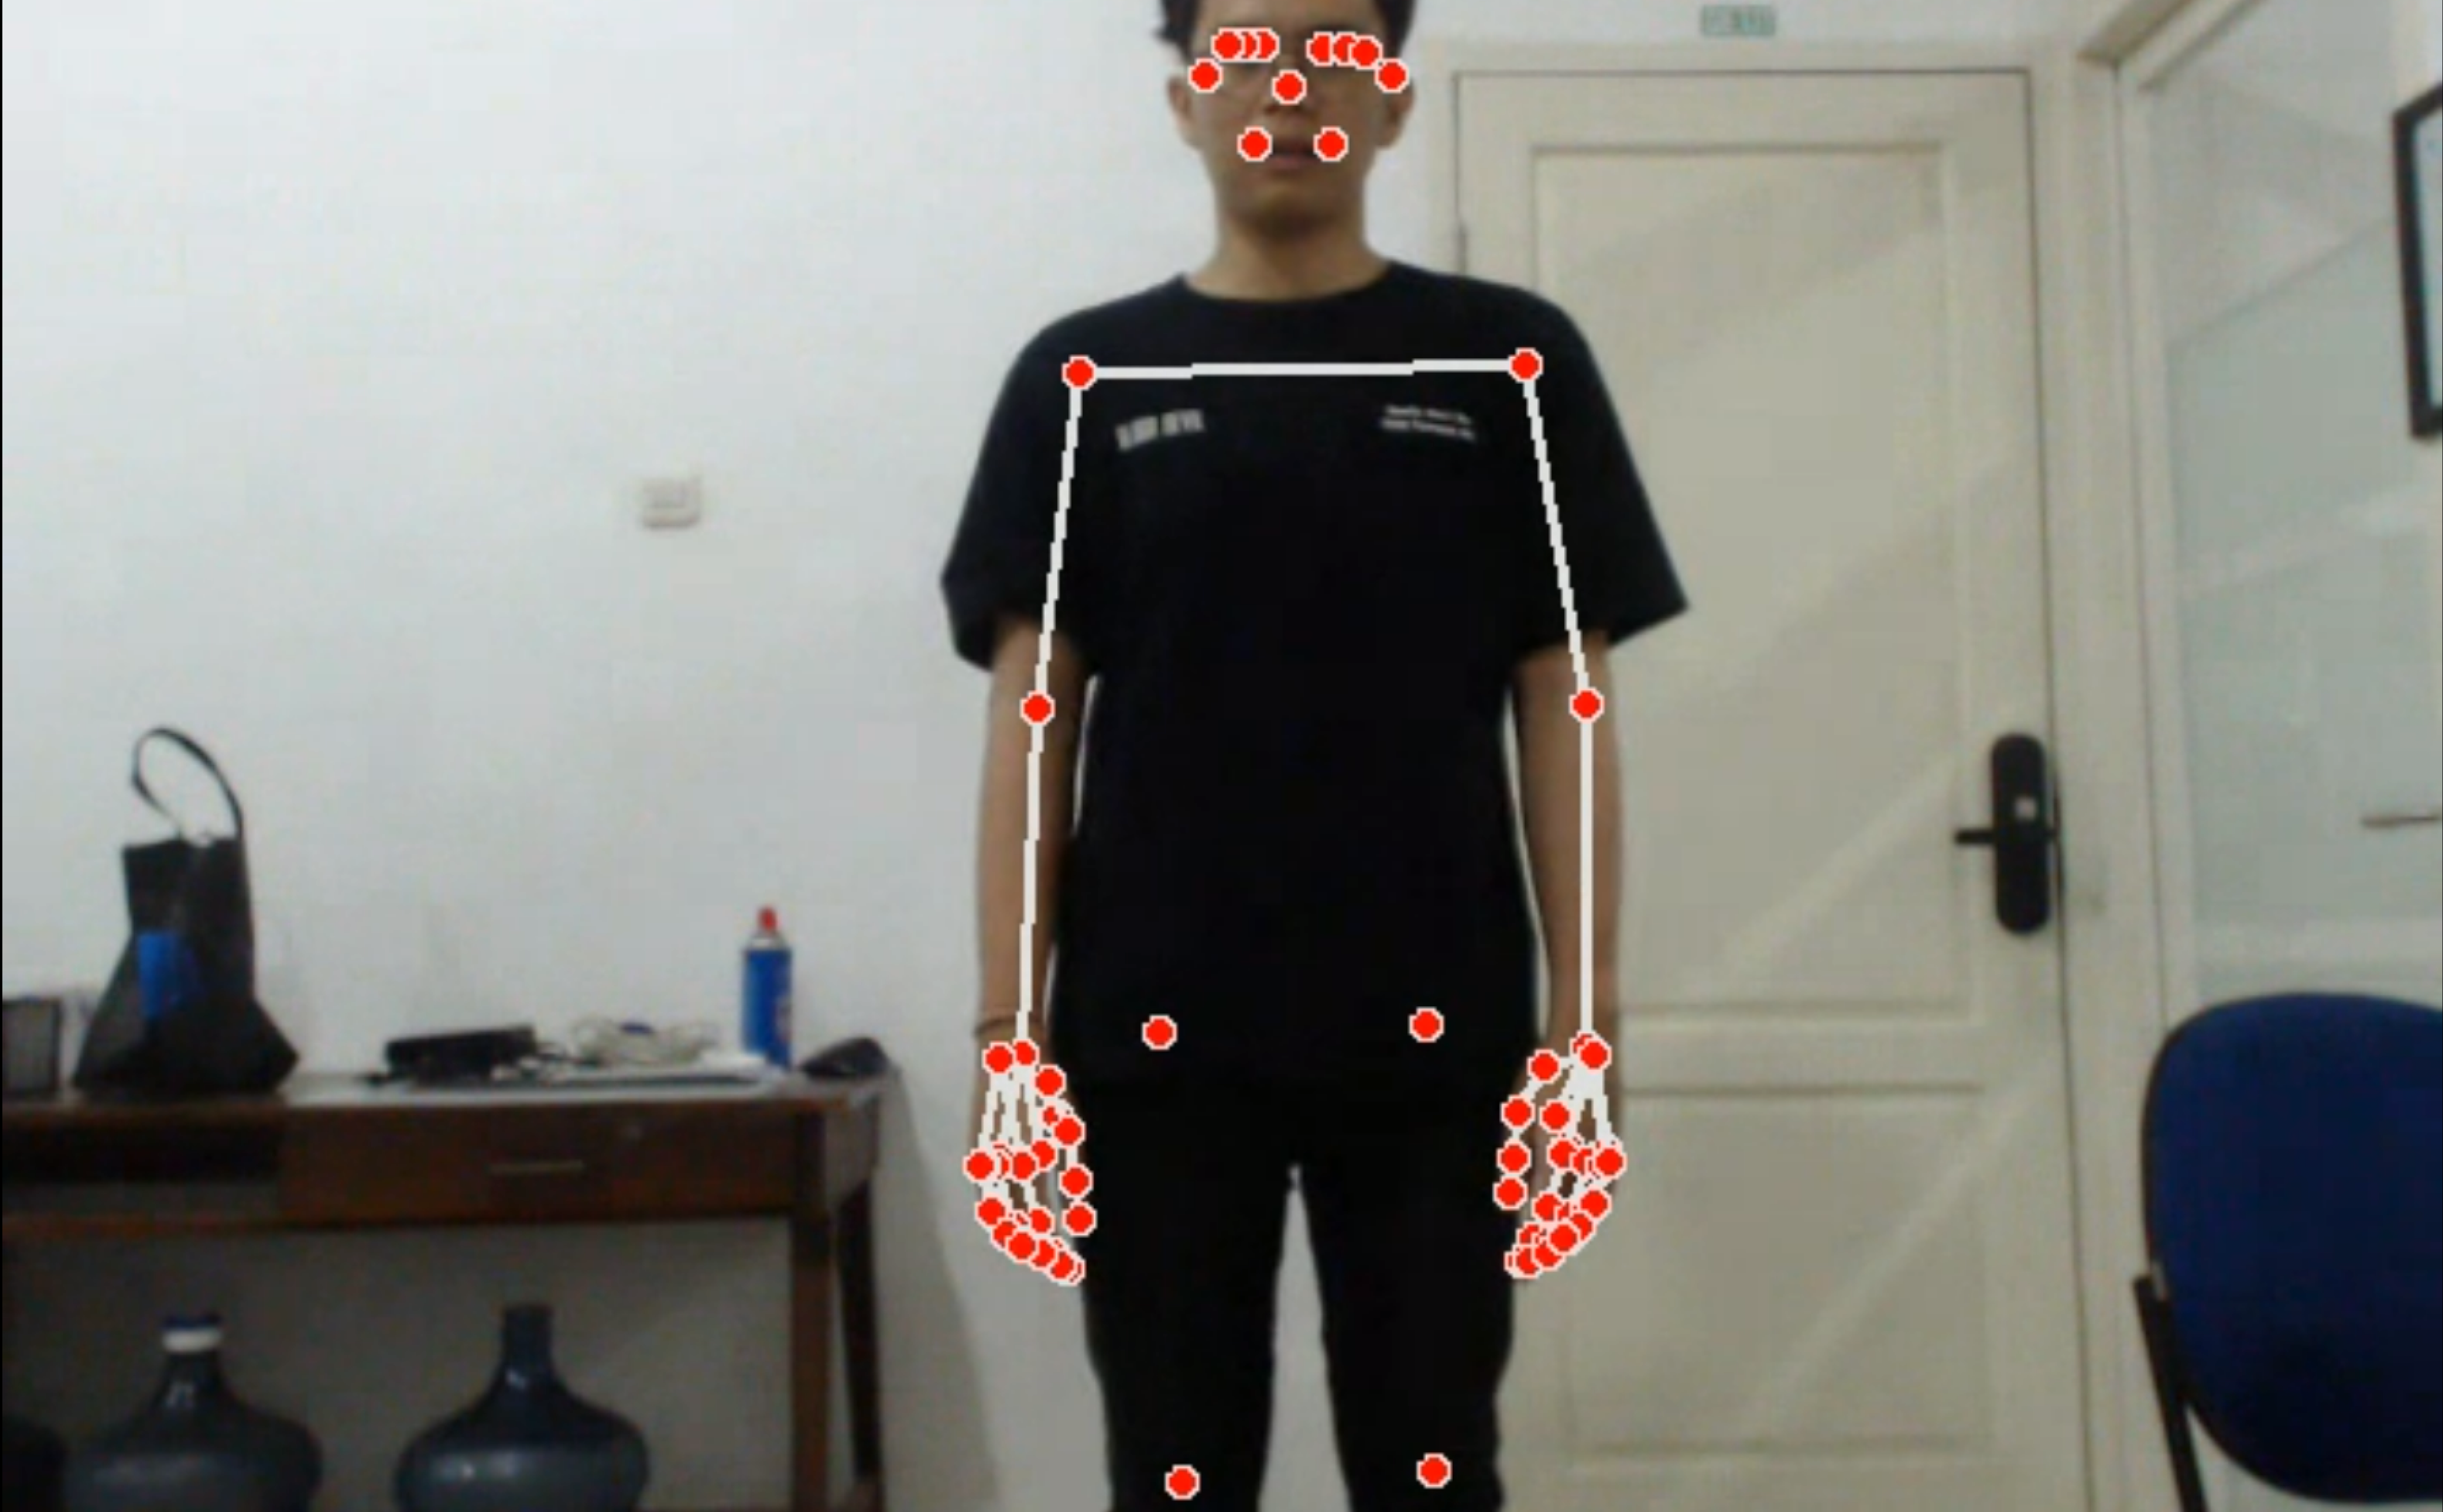
\includegraphics[scale=0.15]{gambar/bab4-jarak300.png}                \\
  \hline
  240 cm            & 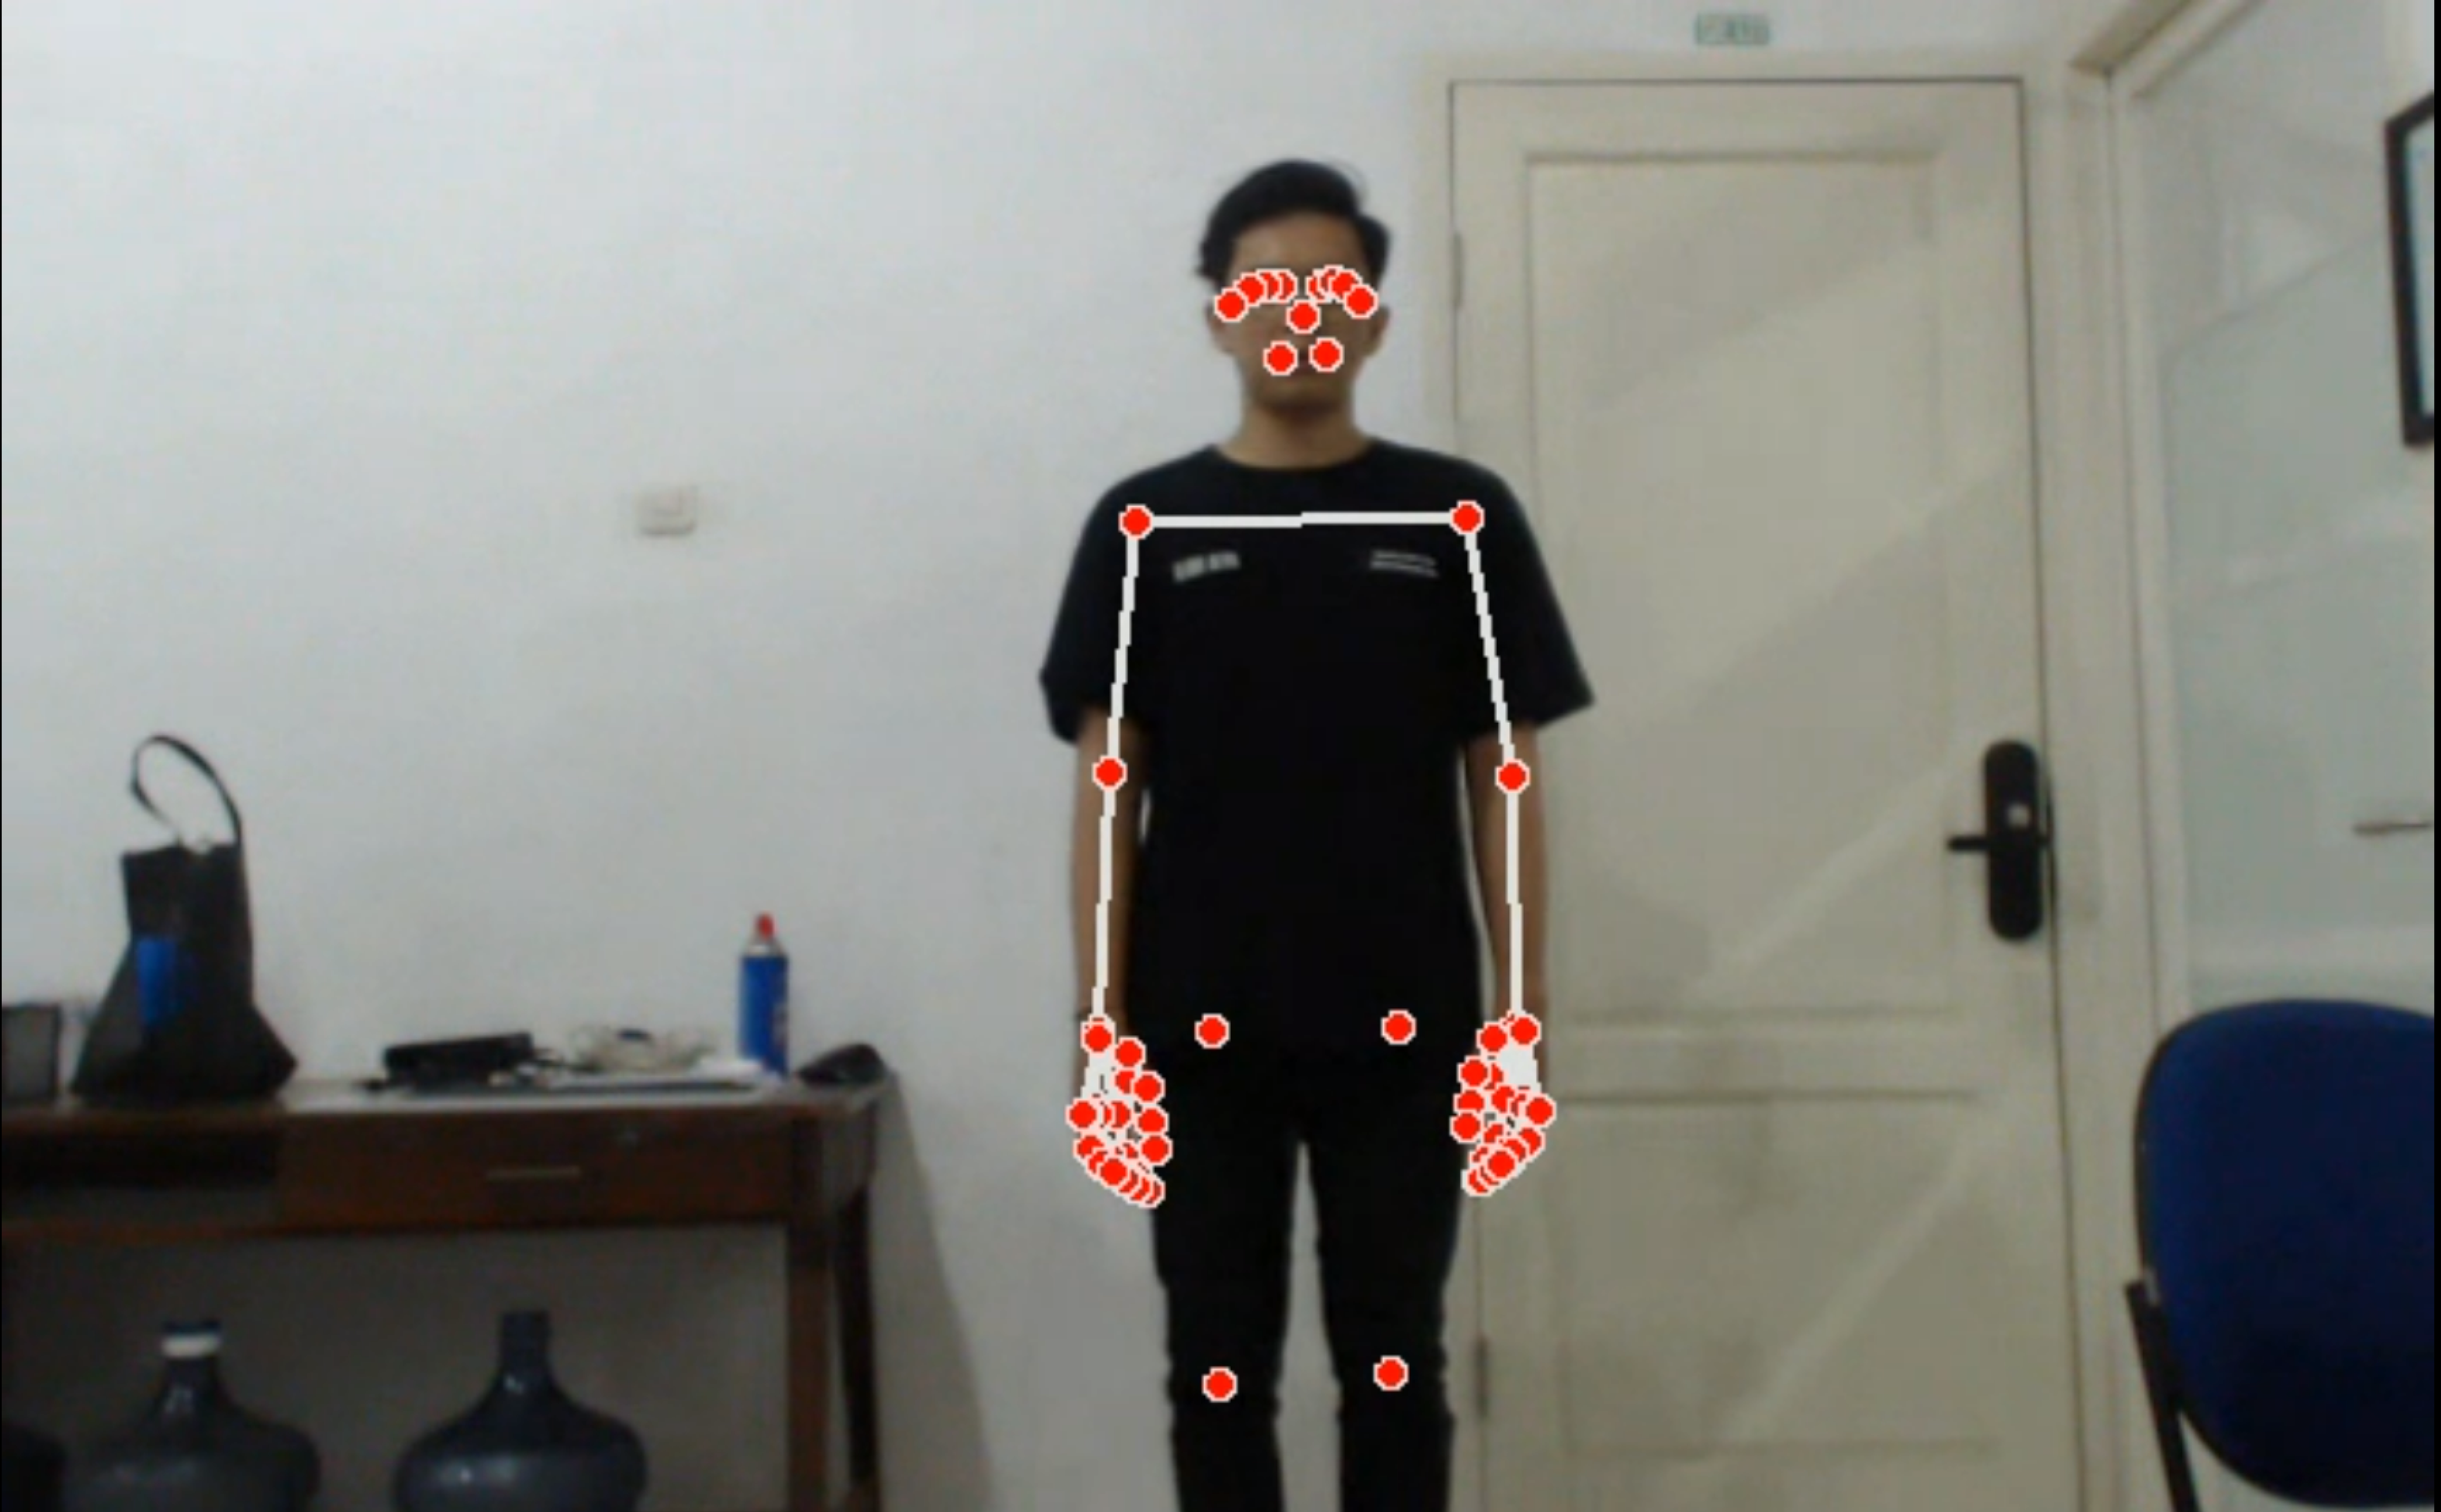
\includegraphics[scale=0.15]{gambar/bab4-jarak240.png}                 \\
  \hline
  300 cm            & 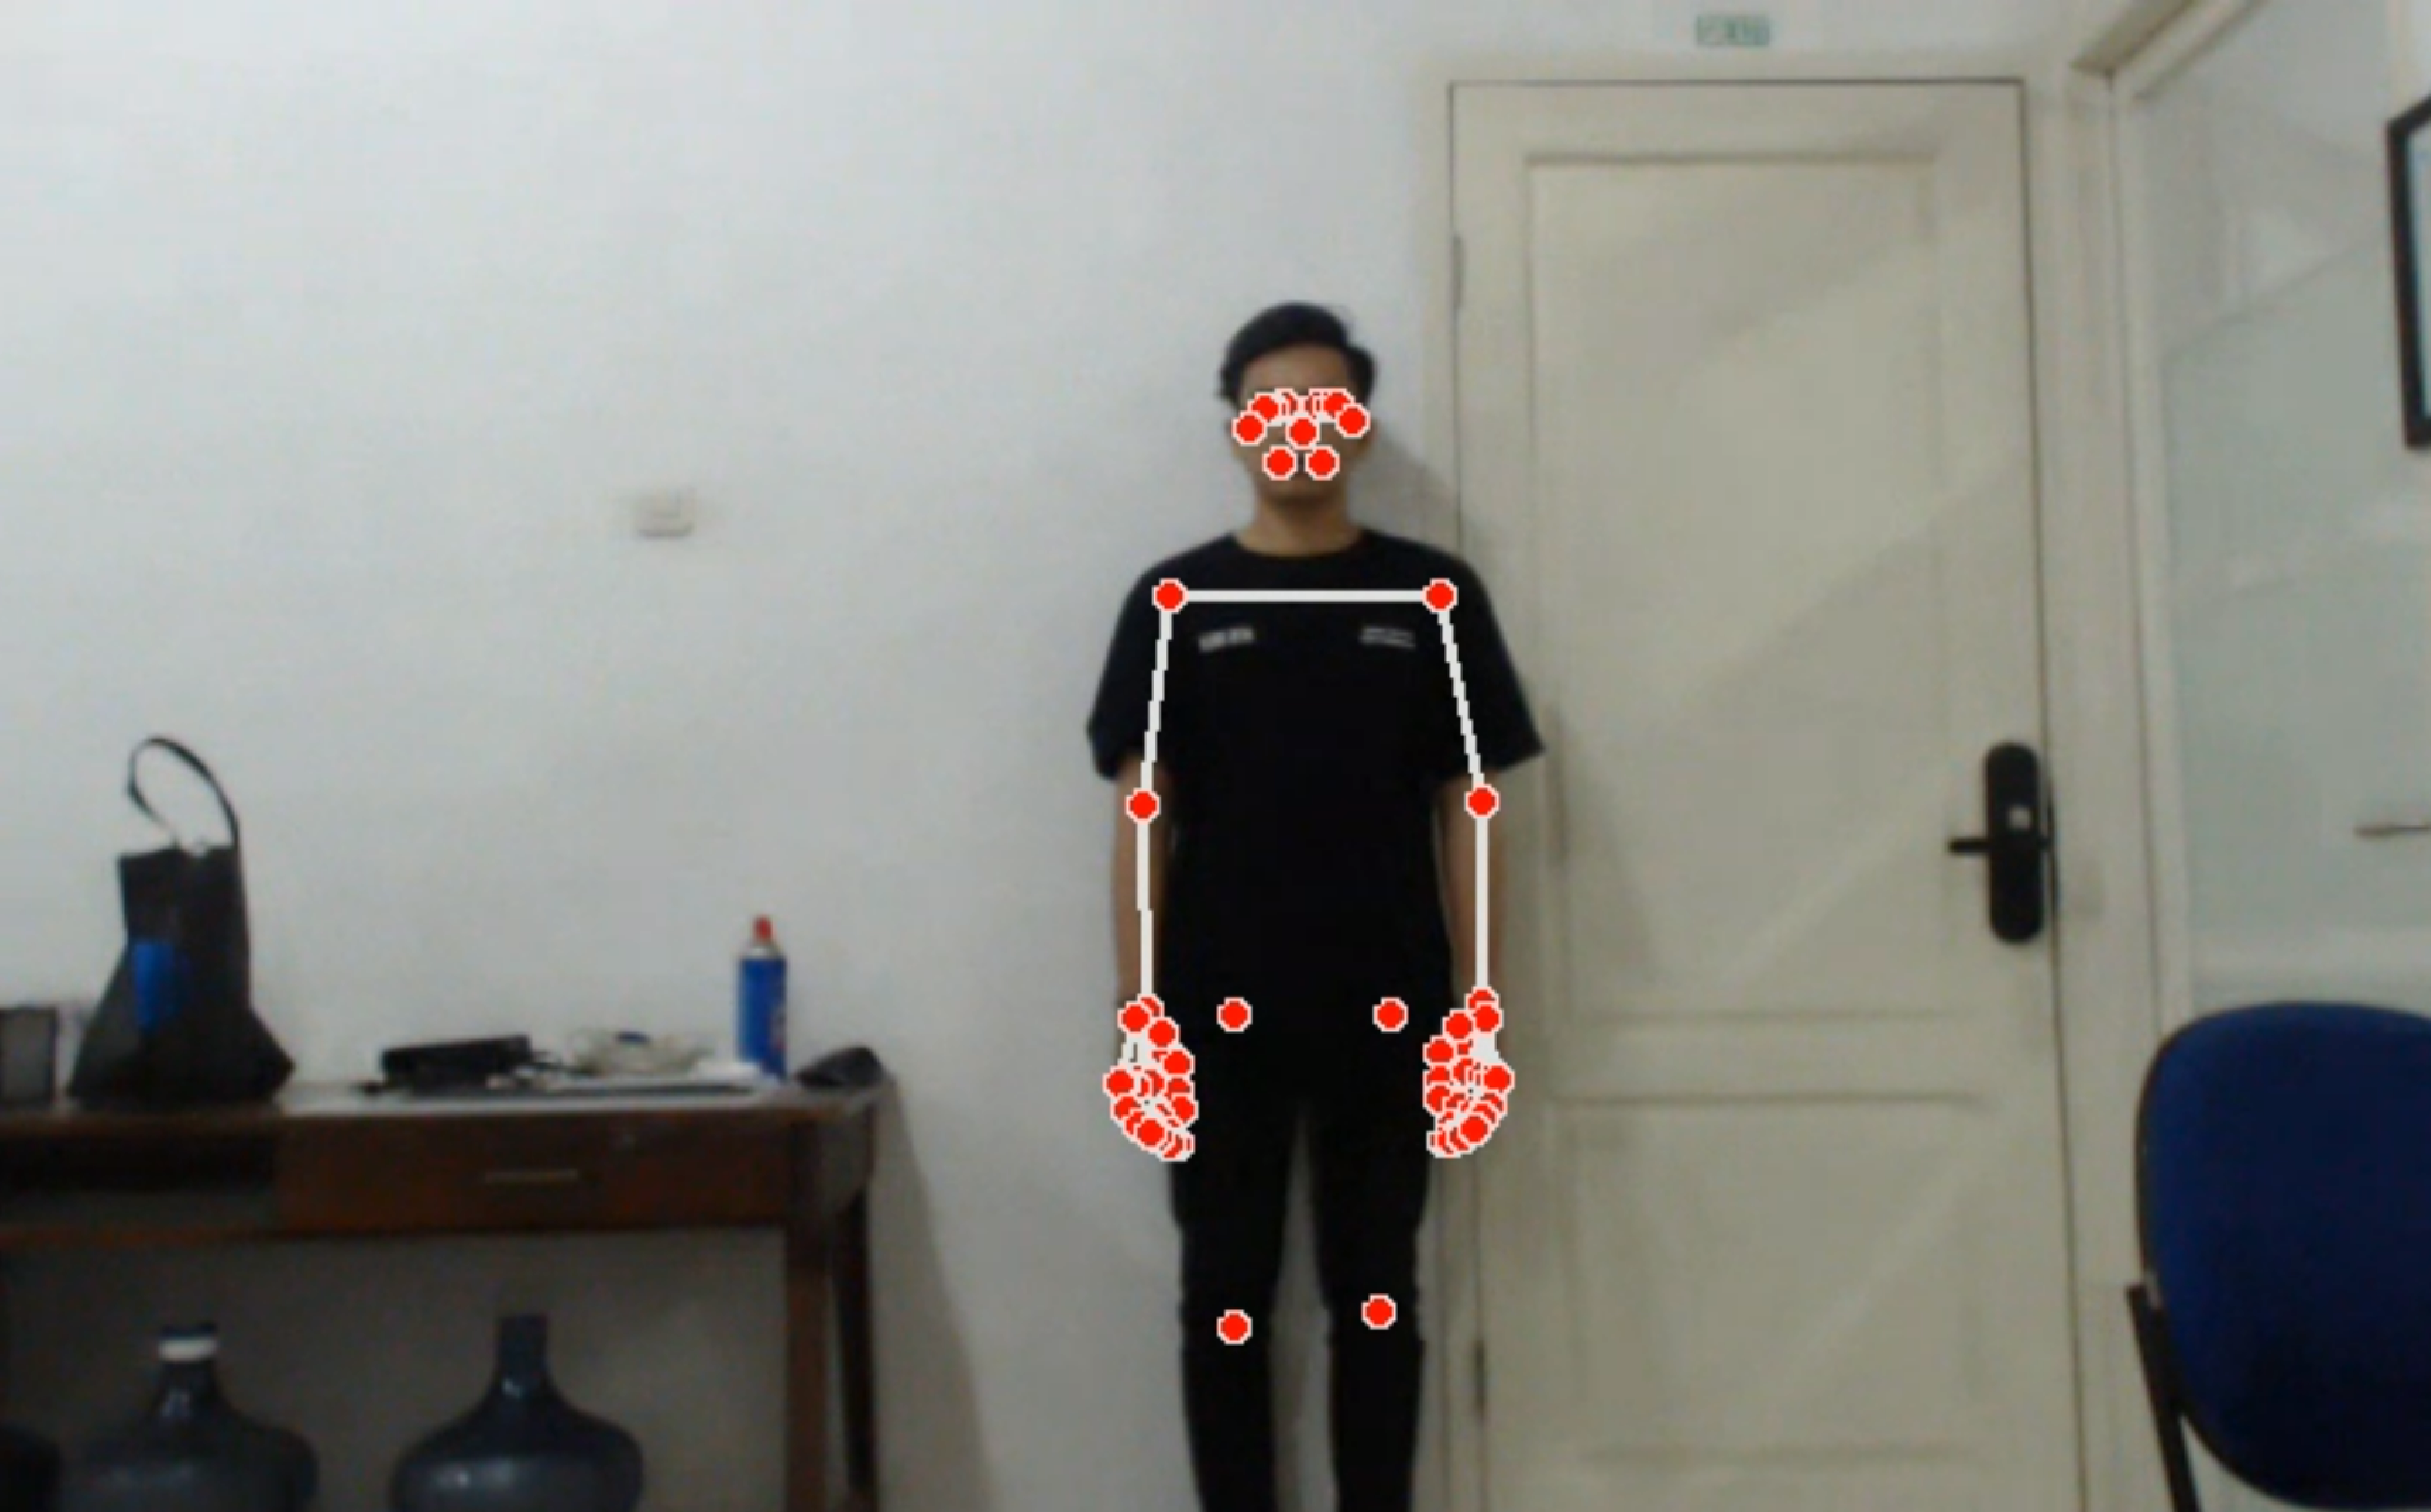
\includegraphics[scale=0.15]{gambar/bab4-jarak180.png}                 \\
  \hline
\end{longtable}

Pada pengujian kondisi jarak ini dilakukan untuk memahami bagaimana performa model pada jarak kamera dengan pengguna yang berbeda - beda. Adapun jarak yang akan digunakan pada pengujian ini adalah 180 cm, 240 cm, dan 300 cm. Variasi jarak ini dipilih dengan mempertimbangkan bahwa bagian kepala hingga tangan pengguna dapat terlihat secara jelas pada kamera sehingga setiap gerakan bahasa isyarat yang akan dilakukan. Untuk menghasilkan klasifikasi model diperlukan 30 \emph{frame} dan untuk setiap \emph{frame} diekstraksi koordinatnya dengan menggunakan \emph{framework} Mediapipe, apabila bagian tubuh pengguna (terkhususnya tangan dan kepala yang dominan digunakan untuk merepresentasikan suatu bahasa isyarat) tidak terlihat pada kamera akan mempengaruhi data koordinat yang didapatkan dan menyulitkan model untuk melakukan klasifikasi dengan tepat. Adapun posisi pengguna dengan jarak masing - masing dapat dlihat pada tabel \ref{tb:kondisijarak}. 

Model penerjemah bahasa Indonesia (BISINDO) yang akan digunakan pada pengujian ini adalah model pada bagian \ref{sec:analisismodel3} karena merupakan model yang menghasilkan klasifikasi yang terbaik jika dibandingkan dengan model lainnya. Untuk setiap variasi jarak akan dilakukan pengujian sebanyak tiga kali dengan kondisi ruangan yang memiliki intensitas cahaya yang terang (berkisar pada 125 lux). Pada setiap pengujian akan dicari hasil klasifikasi model, waktu yang dibutuhkan model untuk menghasilkan klasifikasi bahasa isyarat berdasarkan data koordinat yang diberikan(\emph{processing time}), dan waktu total yang dibutuhkan dalam menghasilkan klasifikasi bahasa isyarat (\emph{complete time}).  

\subsection{Pengujian Jarak 180 cm}
\label{sec:analisisjarak1}

\begin{longtable}{|c|c|c|c|}
  \caption{Pengujian Pertama Model di Kondisi Jarak 180 cm}
  \label{tb:prediksipendek1}                                   \\
  \hline
  \rowcolor[HTML]{C0C0C0}
  \textbf{Kosakata} & \textbf{Klasifikasi Model} & \textbf{\emph{Processing Time}} & \textbf{\emph{Complete Time}}\\
  \hline
  Maaf              & Maaf                          & 0.09432005882263184 detik                          & 2.6262545585632324 detik                                 \\
  Tolong            & Tolong                        & 0.09578323364257812 detik                          & 2.7582406997680664 detik                                 \\
  Nama              & Nama                          & 0.0936741828918457 detik                           & 2.7642273902893066 detik                                 \\
  Saya              & Saya                          & 0.09214234352111816 detik                          & 1.4595723152160645 detik                                 \\
  Siapa              & Siapa                        & 0.09187936782836914 detik                          & 2.6860642433166504 detik                                 \\
  Rumah             & \textcolor{red}{Delete}       & 0.09518122673034668 detik                          & 2.7240443229675293 detik                                 \\
  Delete            & Delete                        & 0.09378981590270996 detik                          & 1.4715027809143066 detik                                 \\
  Standby           & Standby                       & 0.09064006805419922 detik                          & 1.4081025123596191 detik                                 \\
  Translate         & Translate                     & 0.09035801887512207 detik                          & 2.901949882507324 detik                                \\
  \hline
\end{longtable}

\begin{longtable}{|c|c|c|c|}
  \caption{Pengujian Kedua Model di Kondisi Jarak 180 cm}
  \label{tb:prediksipendek2}                                   \\
  \hline
  \rowcolor[HTML]{C0C0C0}
  \textbf{Kosakata} & \textbf{Klasifikasi Model} & \textbf{\emph{Processing Time}} & \textbf{\emph{Complete Time}}\\
  \hline
  Maaf              & \textcolor{red}{Tolong}       & 0.1025094985961914  detik                           & 2.683281898498535  detik                                 \\
  Tolong            & Tolong                        & 0.10531425476074219 detik                           & 2.6761865615844727 detik                                  \\
  Nama              & Nama                          & 0.10347270965576172 detik                           & 2.837998867034912  detik                                 \\
  Saya              & Saya                          & 0.10077977180480957 detik                           & 1.6065859794616701 detik                                  \\
  Siapa              & Siapa                        & 0.09792852401733398 detik                           & 2.89107084274292   detik                                \\
  Rumah             & Rumah                         & 0.09961485862731934 detik                           & 2.9763364791870117 detik                                  \\
  Delete            & Delete                        & 0.10204243659973145 detik                           & 1.4318633079528809 detik                                  \\
  Standby           & Standby                       & 0.10916757583618164 detik                           & 1.4253973960876465 detik                                  \\
  Translate         & Translate                     & 0.1098337173461914  detik                           & 3.0064201354980464 detik                                  \\
  \hline
\end{longtable}

\newpage
\begin{longtable}{|c|c|c|c|}
  \caption{Pengujian Ketiga Model di Kondisi Jarak 180 cm}
  \label{tb:prediksipendek3}                                   \\
  \hline
  \rowcolor[HTML]{C0C0C0}
  \textbf{Kosakata} & \textbf{Klasifikasi Model} & \textbf{\emph{Processing Time}} & \textbf{\emph{Complete Time}}\\
  \hline
  Maaf              & Maaf                          & 0.09703993797302246 detik                          & 2.6079654693603516 detik                                  \\
  Tolong            & Tolong                        & 0.11110496520996094 detik                          & 2.688016891479492 detik                                \\
  Nama              & Nama                          & 0.11299991607666016 detik                          & 2.854478359222412 detik                                \\
  Saya              & Saya                          & 0.1057591438293457 detik                           & 1.4061927795410156 detik                                 \\
  Siapa             & Siapa                         & 0.10792779922485352 detik                          & 2.819080352783203 detik                                \\
  Rumah             & Rumah                         & 0.10235428810119629 detik                          & 2.8994321823120117 detik                                 \\
  Delete            & Delete                        & 0.10874819755554199 detik                          & 1.3875889778137207 detik                                 \\
  Standby           & Standby                       & 0.11034560203552246 detik                          & 1.3965654373168945 detik                                 \\
  Translate         & Translate                     & 0.10168957710266113 detik                          & 3.110654354095459 detik                                \\
  \hline
\end{longtable}

Berdasarkan tiga pengujian yang dilakukan, didapatkan bahwa hampir keseluruhan klasifikasi model yang sesuai dengan \emph{class} kosakata. Namun, terdapat beberapa kesalahan model dalam melakukan klasifikasi. Dapat dilihat pada tabel \ref{tb:prediksipendek1} untuk isyarat kosakata "Rumah" diklasifikasikan sebagai "Delete" dan pada tabel \ref{tb:prediksipendek2} untuk isyarat kosakata "Maaf" diklasifikasikan sebagai "Tolong". Adanya kemiripan antara kosakata menjadi penyebab utama terjadinya kesalahan ini. Kosakata "Rumah" dan "Delete" memiliki kemiripan pada gerakan isyaratnya, dimana kedua kosakata ini sama - sama menggunakan dua tangan dengan gerakan yang mayoritas terjadi pada bagian badan pengguna. Sedangkan untuk kosakata "Maaf" dan "Tolong" memiliki kemiripan pada gerakan isyaratnya dengan kedua kosakata sama - sama menggunakan tangan kanan dengan gerakan akhir yang mayoritas terjadi pada bagian samping wajah pengguna. Namun kemiripan ini tidak sepenuhnya membuat hasil klasifikasi menjadi lebih condong ke suatu kosakata, melainkan dengan pengguna yang memperagakan bahasa isyarat dengan mengutamakan "ciri khas" dari masing - masing bahasa isyarat dapat menghasilkan hasil klasifikasi model yang baik. Hal ini dapat dilihat pada tabel \ref{tb:prediksipendek2} menghasilkan keseluruhan klasifikasi yang benar untuk seluruh \emph{class} kosakata. Pada pengujian dengan kondisi jarak 180 cm, berdasarkan data pda tabel \ref{tb:prediksipendek1}, tabel tabel \ref{tb:prediksipendek2}, dan tabel tabel \ref{tb:prediksipendek3} menunjukkan bahwa model memiliki akurasi klasifikasi sebesar 92.5\%.

Apabila dilihat berdasarkan waktu pemrosesan, rata - rata waktu yang dibutuhkan model untuk menghasilkan klasifikasi bahasa isyarat (\emph{processing time}) adalah 0.101 detik dan rata - rata waktu yang dibutuhkan dalam menghasilkan klasifikasi bahasa isyarat (\emph{complete time}) adalah 2.352 detik. Berdasakan data ini, dapat diamati bahwa model memerlukan waktu yang terbilang singkat dalam memproses serangkaian data koordinat yang diberikan dengan program penerjemah yang mampu menyelesaikan proses klasifikasi dengan cepat untuk sistem yang berjalan secara \emph{real time}. Meskipun dengan kondisi pengguna yang memiliki jarak yang cukup dekat dengan kamera, tidak mempengaruhi secara signifikan terhadap proses klasifikasi bahasa isyarat yang dilakukan oleh model.

Pada pengujian di kondisi jarak 180 cm ini, perlu diperhatikan bahwa pengguna harus melakukan gerakan bahasa isyarat dengan memastikan bahwa bagian tubuh kepala hingga tangan dengan jelas terlihat. Hal ini sangat krusial karena model memerlukan informasi koordinat yang lengkap untuk setiapp gerakan isyarat sehingga dapat menghasilkan klasifikasi yang tepat. Terkhususnya untuk kosakata "Translate", "Maaf", "Tolong", dan "Delete" yang memiliki gerakan isyarat yang cukup dinamis dan mayoritas gerakannya terjadi di samping kepala pengguna.  

\newpage
\subsection{Pengujian Jarak 240 cm}
\label{sec:analisisjarak2}

\begin{longtable}{|c|c|c|c|}
  \caption{Pengujian Pertama Model di Kondisi Jarak 240 cm}
  \label{tb:prediksitengah1}                                   \\
  \hline
  \rowcolor[HTML]{C0C0C0}
  \textbf{Kosakata} & \textbf{Klasifikasi Model} & \textbf{\emph{Processing Time}} & \textbf{\emph{Complete Time}}\\
  \hline
  Maaf              & Maaf                        & 0.09363484382629395 detik                           & 2.8636908531188965 detik                                  \\
  Tolong            & Tolong                      & 0.09594297409057617 detik                           & 2.699732780456543 detik                                \\
  Nama              & Nama                        & 0.0991525650024414 detik                            & 2.716062068939209 detik                                \\
  Saya              & Saya                        & 0.09490489959716797 detik                           & 1.3848638534545898 detik                                 \\
  Siapa             & Siapa                       & 0.09771037101745605 detik                           & 2.778289318084717 detik                                \\
  Rumah             & Rumah                       & 0.09178900718688965 detik                           & 2.8422188758850098 detik                                 \\
  Delete            & Delete                      & 0.09782981872558594 detik                           & 2.746889591217041 detik                                \\
  Standby           & Standby                     & 0.09716463088989258 detik                           & 1.4444875717163086 detik                                 \\
  Translate         & Translate                   & 0.0946202278137207 detik                            & 2.8994321823120117 detik                                 \\
  \hline
\end{longtable}

\begin{longtable}{|c|c|c|c|}
  \caption{Pengujian Kedua Model di Kondisi Jarak 240 cm}
  \label{tb:prediksitengah2}                                   \\
  \hline
  \rowcolor[HTML]{C0C0C0}
  \textbf{Kosakata} & \textbf{Klasifikasi Model} & \textbf{\emph{Processing Time}} & \textbf{\emph{Complete Time}}\\
  \hline
  Maaf              & Maaf                        & 0.10062599182128906 detik                          & 2.837040424346924 detik                                 \\
  Tolong            & Tolong                      & 0.10464692115783691 detik                          & 2.745509147644043 detik                                 \\
  Nama              & Nama                        & 0.0791633129119873 detik                           & 2.7147960662841797 detik                                  \\
  Saya              & Saya                        & 0.11030316352844238 detik                          & 1.4569830894470215 detik                                  \\
  Siapa             & Siapa                       & 0.09940838813781738 detik                          & 2.7176427841186523 detik                                  \\
  Rumah             & Rumah                       & 0.10739994049072266 detik                          & 2.7834320068359375 detik                                  \\
  Delete            & Delete                      & 0.10262727737426758 detik                          & 2.848219871520996 detik                                 \\
  Standby           & Standby                     & 0.10418152809143066 detik                          & 1.4255762100219727 detik                                  \\
  Translate         & Translate                   & 0.10814952850341797 detik                          & 2.913722991943359  detik                                 \\
  \hline
\end{longtable}

\begin{longtable}{|c|c|c|c|}
  \caption{Pengujian Ketiga Model di Kondisi Jarak 240 cm}
  \label{tb:prediksitengah3}                                   \\
  \hline
  \rowcolor[HTML]{C0C0C0}
  \textbf{Kosakata} & \textbf{Klasifikasi Model} & \textbf{\emph{Processing Time}} & \textbf{\emph{Complete Time}}\\
  \hline
  Maaf              & Maaf                          & 0.08161234855651855 detik                           & 2.9344153404235835 detik                                  \\
  Tolong            & Tolong                        & 0.10856509208679199 detik                           & 2.842411994934082 detik                                 \\
  Nama              & Nama                          & 0.08474326133728027 detik                           & 2.8757071495056152 detik                                  \\
  Saya              & Saya                          & 0.10568404197692871 detik                           & 1.7722105979919436 detik                                  \\
  Siapa              & Siapa                        & 0.10201120376586914 detik                           & 2.6211905479431152 detik                                  \\
  Rumah             & \textcolor{red}{Delete}       & 0.10468339920043945 detik                           & 2.7255606651306152 detik                                  \\
  Delete            & Delete                        & 0.1030888557434082 detik                            & 2.8281641006469727 detik                                  \\
  Standby           & Standby                       & 0.10799098014831543 detik                           & 1.4275431632995605 detik                                  \\
  Translate         & Translate                     & 0.10626840591430664 detik                           & 2.813551425933838 detik                                 \\
  \hline
\end{longtable}

Berdasarkan tiga pengujian yang telah dilakukan, didapatkan bahwa hampir keseluruhan klasifikasi model telah sesuai dengan \emph{class} kosakata yang bersesuaian. Hal ini menunjukkan bahwa adanya pengaruh antara jarak pengguna dengan kamera terhadap proses klasifikasi model. Peningkatan jarak pengguna terhadap menghasilkan klasifikasi yang lebih baik. Namun, masih terdapat kesalahan yang dapat dilihat pada tabel \ref{tb:prediksitengah3}, yaitu isyarat kosakata "Rumah" diklasifikasikan sebagai "Delete". Sama seperti yang sudah dijelaskan pada pengujian di kondisi jarak 180 cm bahwa terdapat kemiripan antara kosakata "Rumah" dengan "Delete". Pada pengujian dengan kondisi jarak 240 cm ini, berdasarkan data pada tabel \ref{tb:prediksitengah1}, tabel \ref{tb:prediksitengah2}, dan tabel \ref{tb:prediksitengah3} menunjukkan bahwa model memiliki akurasi klasifikasi sebesar 96.3\%.

Apabila dilihat berdasarkan waktu pemrosesan, rata - rata waktu yang dibutuhkan model untuk menghasilkan klasifikasi bahasa isyarat (\emph{processing time}) adalah 0.099 detik dan rata - rata waktu yang dibutuhkan dalam menghasilkan klasifikasi bahasa isyarat (\emph{complete time}) adalah 2.506 detik. Apabila dibandingkan dengan pengujian sebelumnya (kondisi jarak 180 cm). Terdapat peningkatan pada nilai \emph{processing time} seiring dengan peningkatan jarak kamera dengan pengguna yaitu sebesar 0.002 detik. Sedangkan untuk nilai \emph{complete time} mengalami penurunan seiring dengan peningkatan jarak kamera dengan pengguna, yaitu sebesar 0.154 detik. Hal ini dapat disebabkan oleh adanya pengaruh antara jarak pengguna dengan kamera terhadap bagaimana beban kerja kamera dalam menangkap tiap \emph{frame}.

\subsection{Pengujian Jarak 300 cm}
\label{sec:analisisjarak3}

\begin{longtable}{|c|c|c|c|}
  \caption{Pengujian Pertama Model di Kondisi Jarak 300 cm}
  \label{tb:prediksijauh1}                                   \\
  \hline
  \rowcolor[HTML]{C0C0C0}
  \textbf{Kosakata} & \textbf{Klasifikasi Model} & \textbf{\emph{Processing Time}} & \textbf{\emph{Complete Time}}\\
  \hline
  Maaf              & Maaf                          & 0.09520149230957031 detik                           & 2.738614082336426 detik                                  \\
  Tolong            & Tolong                        & 0.0926811695098877 detik                            & 2.878732681274414 detik                                  \\
  Nama              & Nama                          & 0.0982358455657959 detik                            & 2.915797233581543 detik                                  \\
  Saya              & Saya                          & 0.0943760871887207 detik                            & 2.8119421005249023 detik                                  \\
  Siapa              & Siapa                        & 0.1026923656463623 detik                            & 2.7649641036987305 detik                                  \\
  Rumah             & Rumah                         & 0.09520149230957031 detik                           & 2.740323543548584 detik                                  \\
  Delete            & Delete                        & 0.09269595146179199 detik                           & 2.981078624725342 detik                                  \\
  Standby           & Standby                       & 0.09149551391601562 detik                           & 2.813115119934082 detik                                  \\
  Translate         & Translate                     & 0.09415459632873535 detik                           & 2.848083972930908 detik                                  \\
  \hline
\end{longtable}

\begin{longtable}{|c|c|c|c|}
  \caption{Pengujian Kedua Model di Kondisi Jarak 300 cm}
  \label{tb:prediksijauh2}                                   \\
  \hline
  \rowcolor[HTML]{C0C0C0}
  \textbf{Kosakata} & \textbf{Klasifikasi Model} & \textbf{\emph{Processing Time}} & \textbf{\emph{Complete Time}}\\
  \hline
  Maaf              & Maaf                          & 0.11374950408935547 detik                           & 2.8633904457092285 detik                                  \\
  Tolong            & Tolong                        & 0.10336184501647949 detik                           & 2.7457737922668457 detik                                  \\
  Nama              & Nama                          & 0.1011803150177002 detik                            & 2.690098285675049 detik                                 \\
  Saya              & Saya                          & 0.11127400398254395 detik                           & 2.720317840576172 detik                                 \\
  Siapa              & Siapa                        & 0.10362887382507324 detik                           & 2.84954309463501 detik                                \\
  Rumah             & Rumah                         & 0.10374069213867188 detik                           & 2.8711438179016113 detik                                  \\
  Delete            & Delete                        & 0.10743093490600586 detik                           & 2.7329492568969727 detik                                  \\
  Standby           & Standby                       & 0.10061454772949219 detik                           & 2.903716564178467 detik                                 \\
  Translate         & Translate                     & 0.10336613655090332 detik                           & 2.752346992492676 detik                                 \\
  \hline
\end{longtable}

\newpage
\begin{longtable}{|c|c|c|c|}
  \caption{Pengujian Ketiga Model di Kondisi Jarak 300 cm}
  \label{tb:prediksijauh3}                                   \\
  \hline
  \rowcolor[HTML]{C0C0C0}
  \textbf{Kosakata} & \textbf{Klasifikasi Model} & \textbf{\emph{Processing Time}} & \textbf{\emph{Complete Time}}\\
  \hline
  Maaf              & Maaf                        & 0.09520149230957031 detik                          & 2.7579760551452637 detik                                 \\
  Tolong            & Tolong                      & 0.0926811695098877 detik                          & 2.6619672775268555 detik                                 \\
  Nama              & Nama                        & 0.0982358455657959 detik                          & 2.8861284255981445 detik                                 \\
  Saya              & Saya                        & 0.0943760871887207 detik                          & 2.800147533416748 detik                                 \\
  Siapa             & Siapa                       & 0.1026923656463623 detik                          & 2.763504981994629 detik                                 \\
  Rumah             & Rumah                       & 0.09520149230957031 detik                          & 2.811462879180908 detik                                  \\
  Delete            & Delete                      & 0.09269595146179199 detik                          & 2.6989388465881348 detik                                 \\
  Standby           & Standby                     & 0.09675002098083496 detik                          & 2.7558088302612305 detik                                  \\
  Translate         & Translate                   & 0.10323047637939453 detik                          & 2.67941951751709 detik                                  \\
  \hline
\end{longtable}

Berdasarkan tiga pengujian yang telah dilakukan, didapatkan bahwa keseluruhan klasifikasi model yang sesuai dengan \emph{class} kosakata. Hal ini menunjukkan bahwa peningkatan jarak berpengaruh pada proses klasifikasi yang dilakukan oleh model. Peningkatan jarak antara pengguna dengan kamera, terkhususnya pada jarak terjauh pada pengujian ini, menghasilkan klasifikasi yang lebih baik dan tepat sesuai dengan kosakata yang bersesuaian dengan gerakannya. Hal ini dapat disebabkan oleh semakin jauh jarak antara kamera dengan pengguna memudahkan dalam memproses pose pengguna sehingga menghasilkan data koordinat yang lebih baik lagi. Berdasarkan data pada tabel \ref{tb:prediksijauh1}, tabel \ref{tb:prediksijauh2}, tabel \ref{tb:prediksijauh3} menunjukkan bahwa model memiliki akurasi klasifikasi sebesar 100\%.

Apabila dilihat berdasarkan waktu pemrosesan, rata - rata waktu yang dibutuhkan model untuk menghasilkan klasifikasi bahasa isyarat (\emph{processing time}) adalah 0.099 detik dan rata - rata waktu yang dibutuhkan dalam menghasilkan klasifikasi bahasa isyarat (\emph{complete time}) adalah 2.794 detik. Dapat dilihat bahwa tidak terdapat peningkatan pada \emph{processing time} jika dibandingkan dengan variasi jarak pada pengujian sebelumnya. Namun, pada nilai \emph{complete time} terdapat penurunan jika dibandingkan dengan pengujian sebelumnya, yaitu sebesar 0.288 detik. Hal ini menunjukkan bahwa terdapat penurunan dari nilai \emph{complete time} seiring dengan peningkatan jarak kamera dengan pengguna. Hal ini dapat kembali lagi menguatkan bahwa adanya pengaruh antara jarak pengguna dengan kamera terhadap bagaimana beban kerja kamera dalam menangkap tiap \emph{frame}.

\subsection{Rangkuman Pengujian Kondisi Jarak}
\label{sec:analisisrangkumanjarak}

\begin{longtable}{|c|c|c|c|}
  \caption{Rangkuman Pengujian Kondisi Jarak}
  \label{tb:evaluasiJarak}                                   \\
  \hline
  \rowcolor[HTML]{C0C0C0}
  \textbf{Jarak} & \textbf{Akurasi} & \emph{\textbf{Avg. Processing Time}} & \emph{\textbf{Avg. Complete Time}} \\
  \hline
  180 cm & 0.89 & 0.1017 detik & 2.3660 detik \\
  240 cm & 0.96 & 0.0994 detik & 2.5098 detik \\
  300 cm & 1.00 & 0.0997 detik & 2.7918 detik \\
  \hline
\end{longtable}

Secara keseluruhan, dapat dilihat pada tabel \ref{tb:evaluasiJarak} bahwa variasi jarak yang berbeda tidak berpengaruh secara signifikan terhadap hasil klasifikasi model. Hal ini menunjukkan bahwa metode normalisasi data yang digunakan telah berhasil menghasilkan model yang invarian terhadap jarak. Dengan catatan bahwa posisi pengguna (terkhususnya bagian kepala dan tangan) dapat dengan jelas terlihat ketika melakukan gerakan isyarat. Dapat dilihat bahwa ada relasi antara jarak dengan \emph{average complete time}. Peningkatan \emph{average}. Namun, pada nilai \emph{average processing time} cenderung menurun dengan adanya peningkatan jarak. Kemampuan kamera dalam menangkap \emph{frame} menjadi pengaruh utama dalam peningkatan nilai \emph{complete time} dan \emph{processing time} karena gerakan isyarat yang dinamis memerlukan posisi kamera yang dapat menangkap setiap gerakan dengan jelas dan tepat. Semakin jelas gerakan isyarat yang ditangkap akan memudahkan \emph{framework} Mediapipe dalam mendapatkan data koordinat berdasarkan \emph{landmark} yang ada. Hal ini tentunya akan meningkatkan akurasi klasifikasi model, dimana ditunjukkan dengan adanya peningkatan akurasi seiring dengan peningkatan jarak.

\section{Pengujian Subjek Berbeda}
\label{sec:analisissubjek}

\begin{longtable}{|c|c|}
  \caption{Variasi Subjek Berbeda}
  \label{tb:kondisisubjek}                                   \\
  \hline
  \rowcolor[HTML]{C0C0C0}
  \textbf{Jenis Kelamin} & \textbf{Gambar Subjek}  \\
  \hline
  Perempuan            &  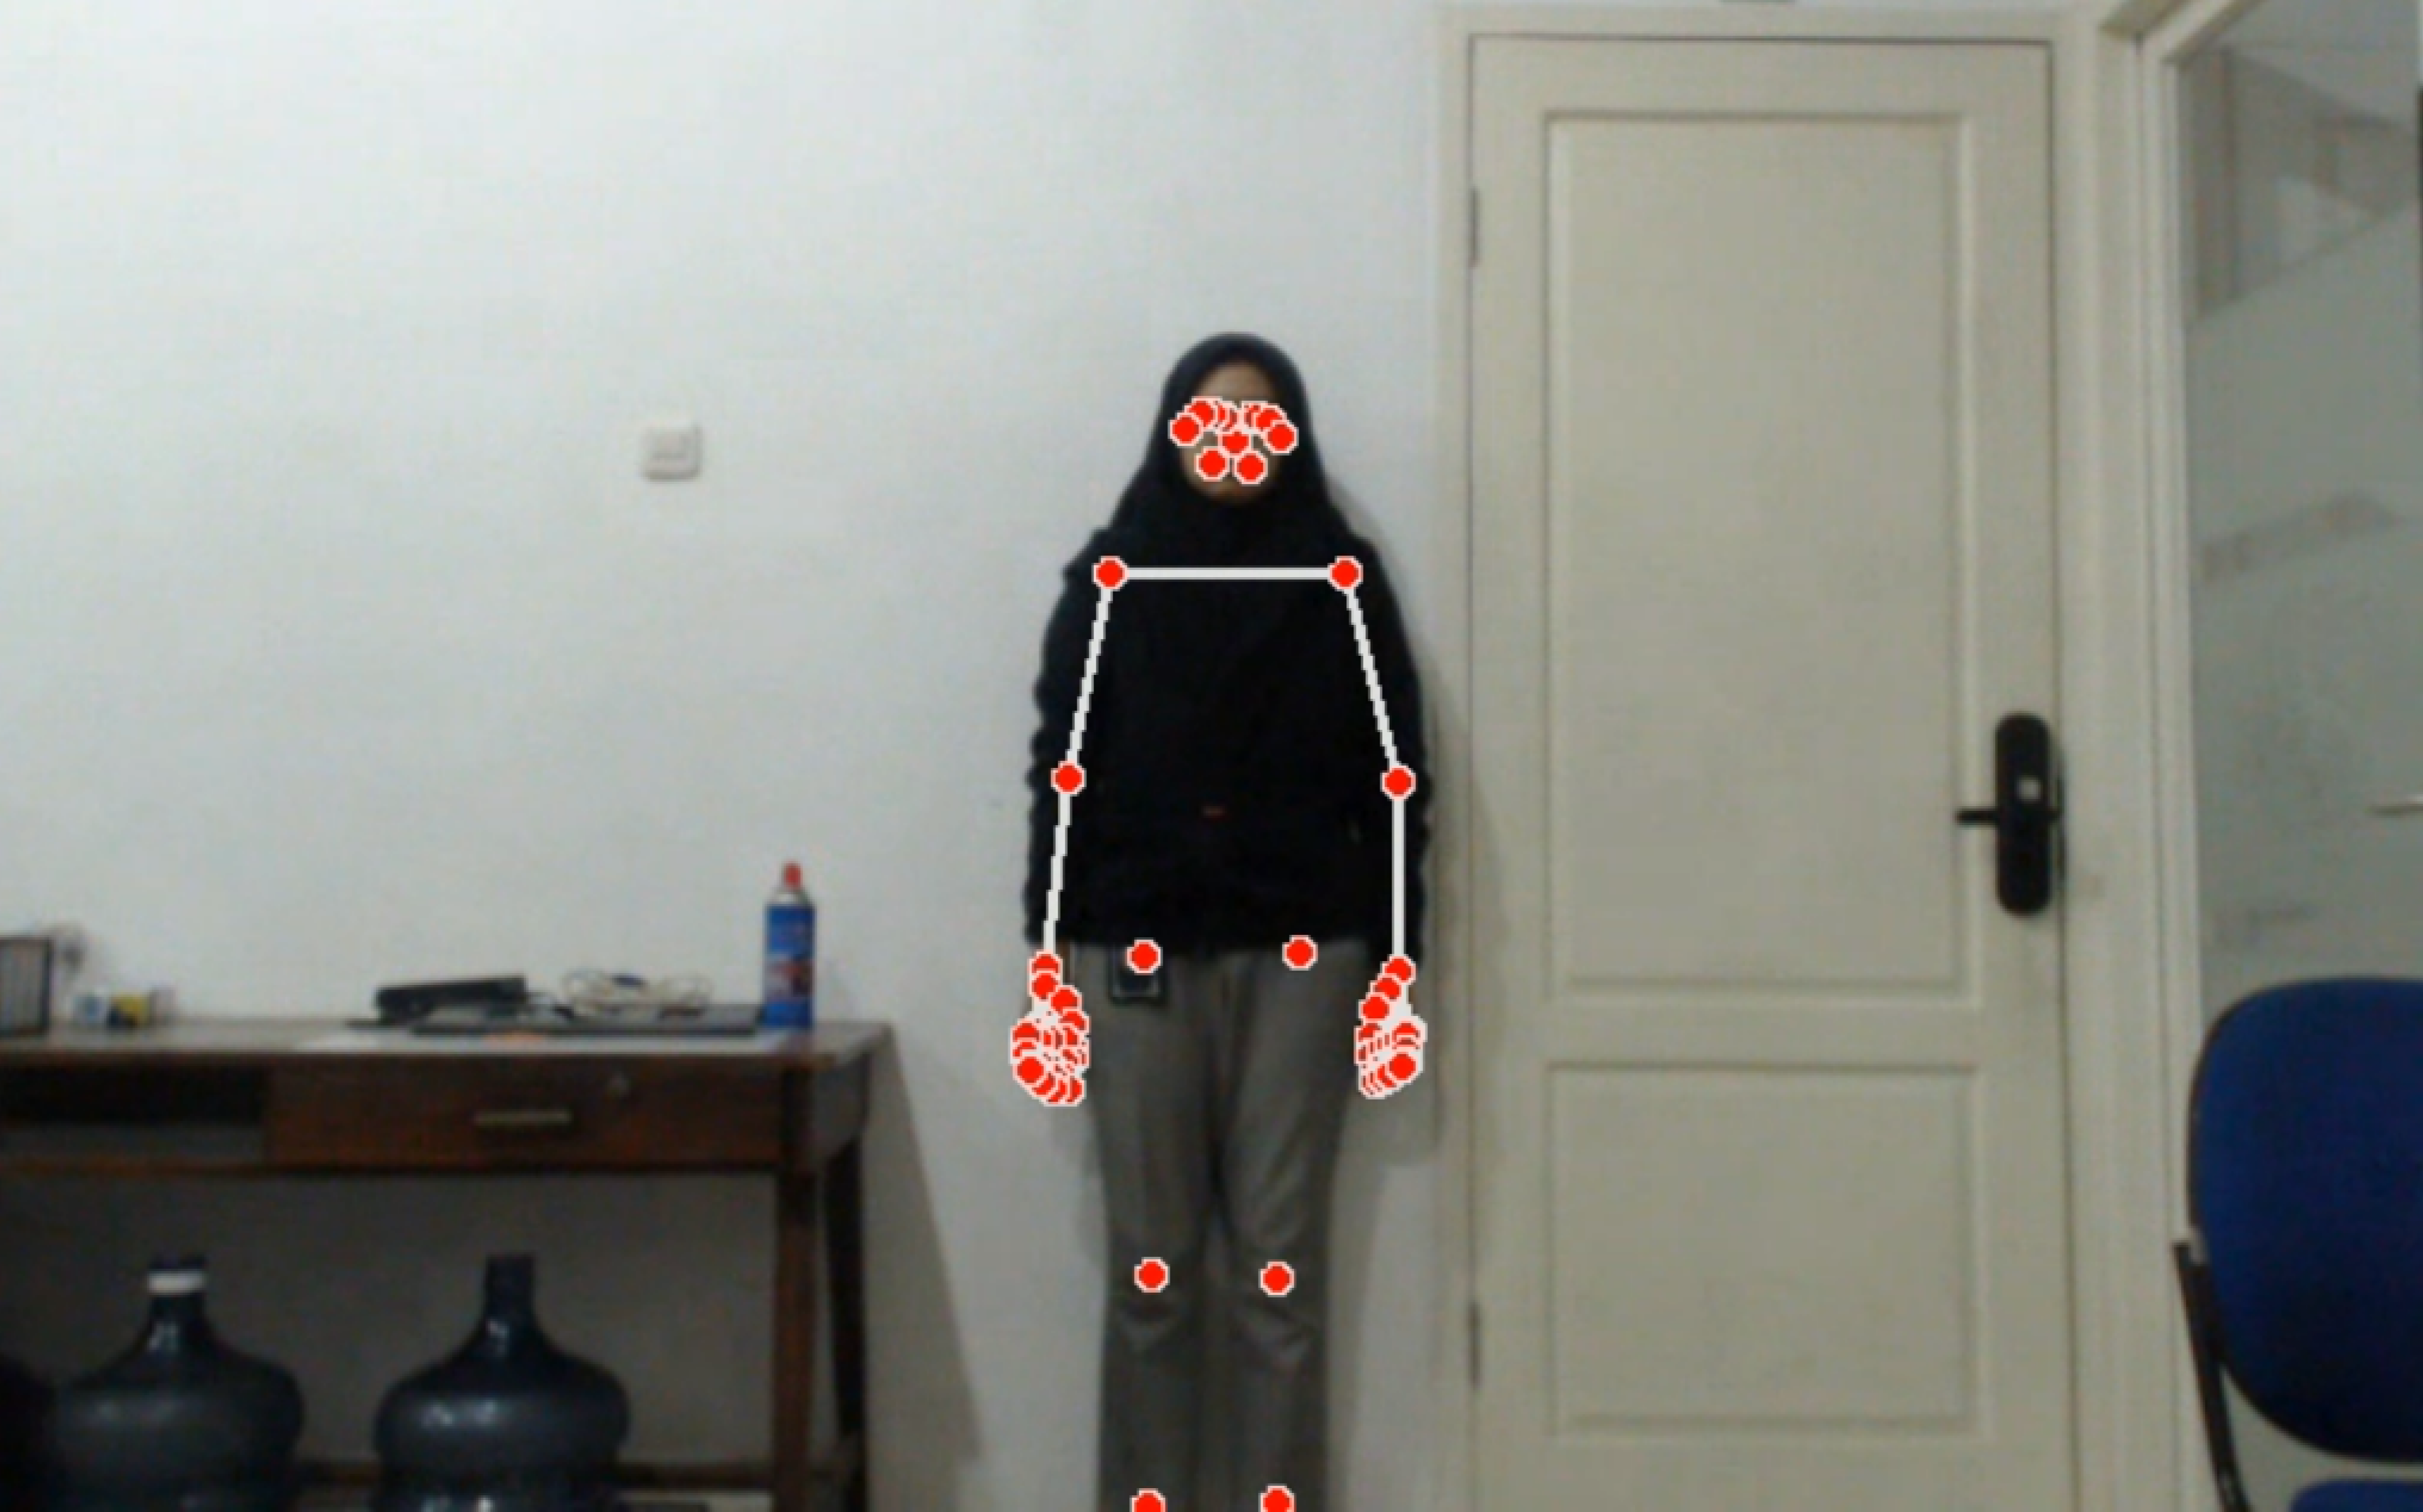
\includegraphics[scale=0.3]{gambar/bab4-rani.png}                \\
  \hline
  Laki - Laki            & 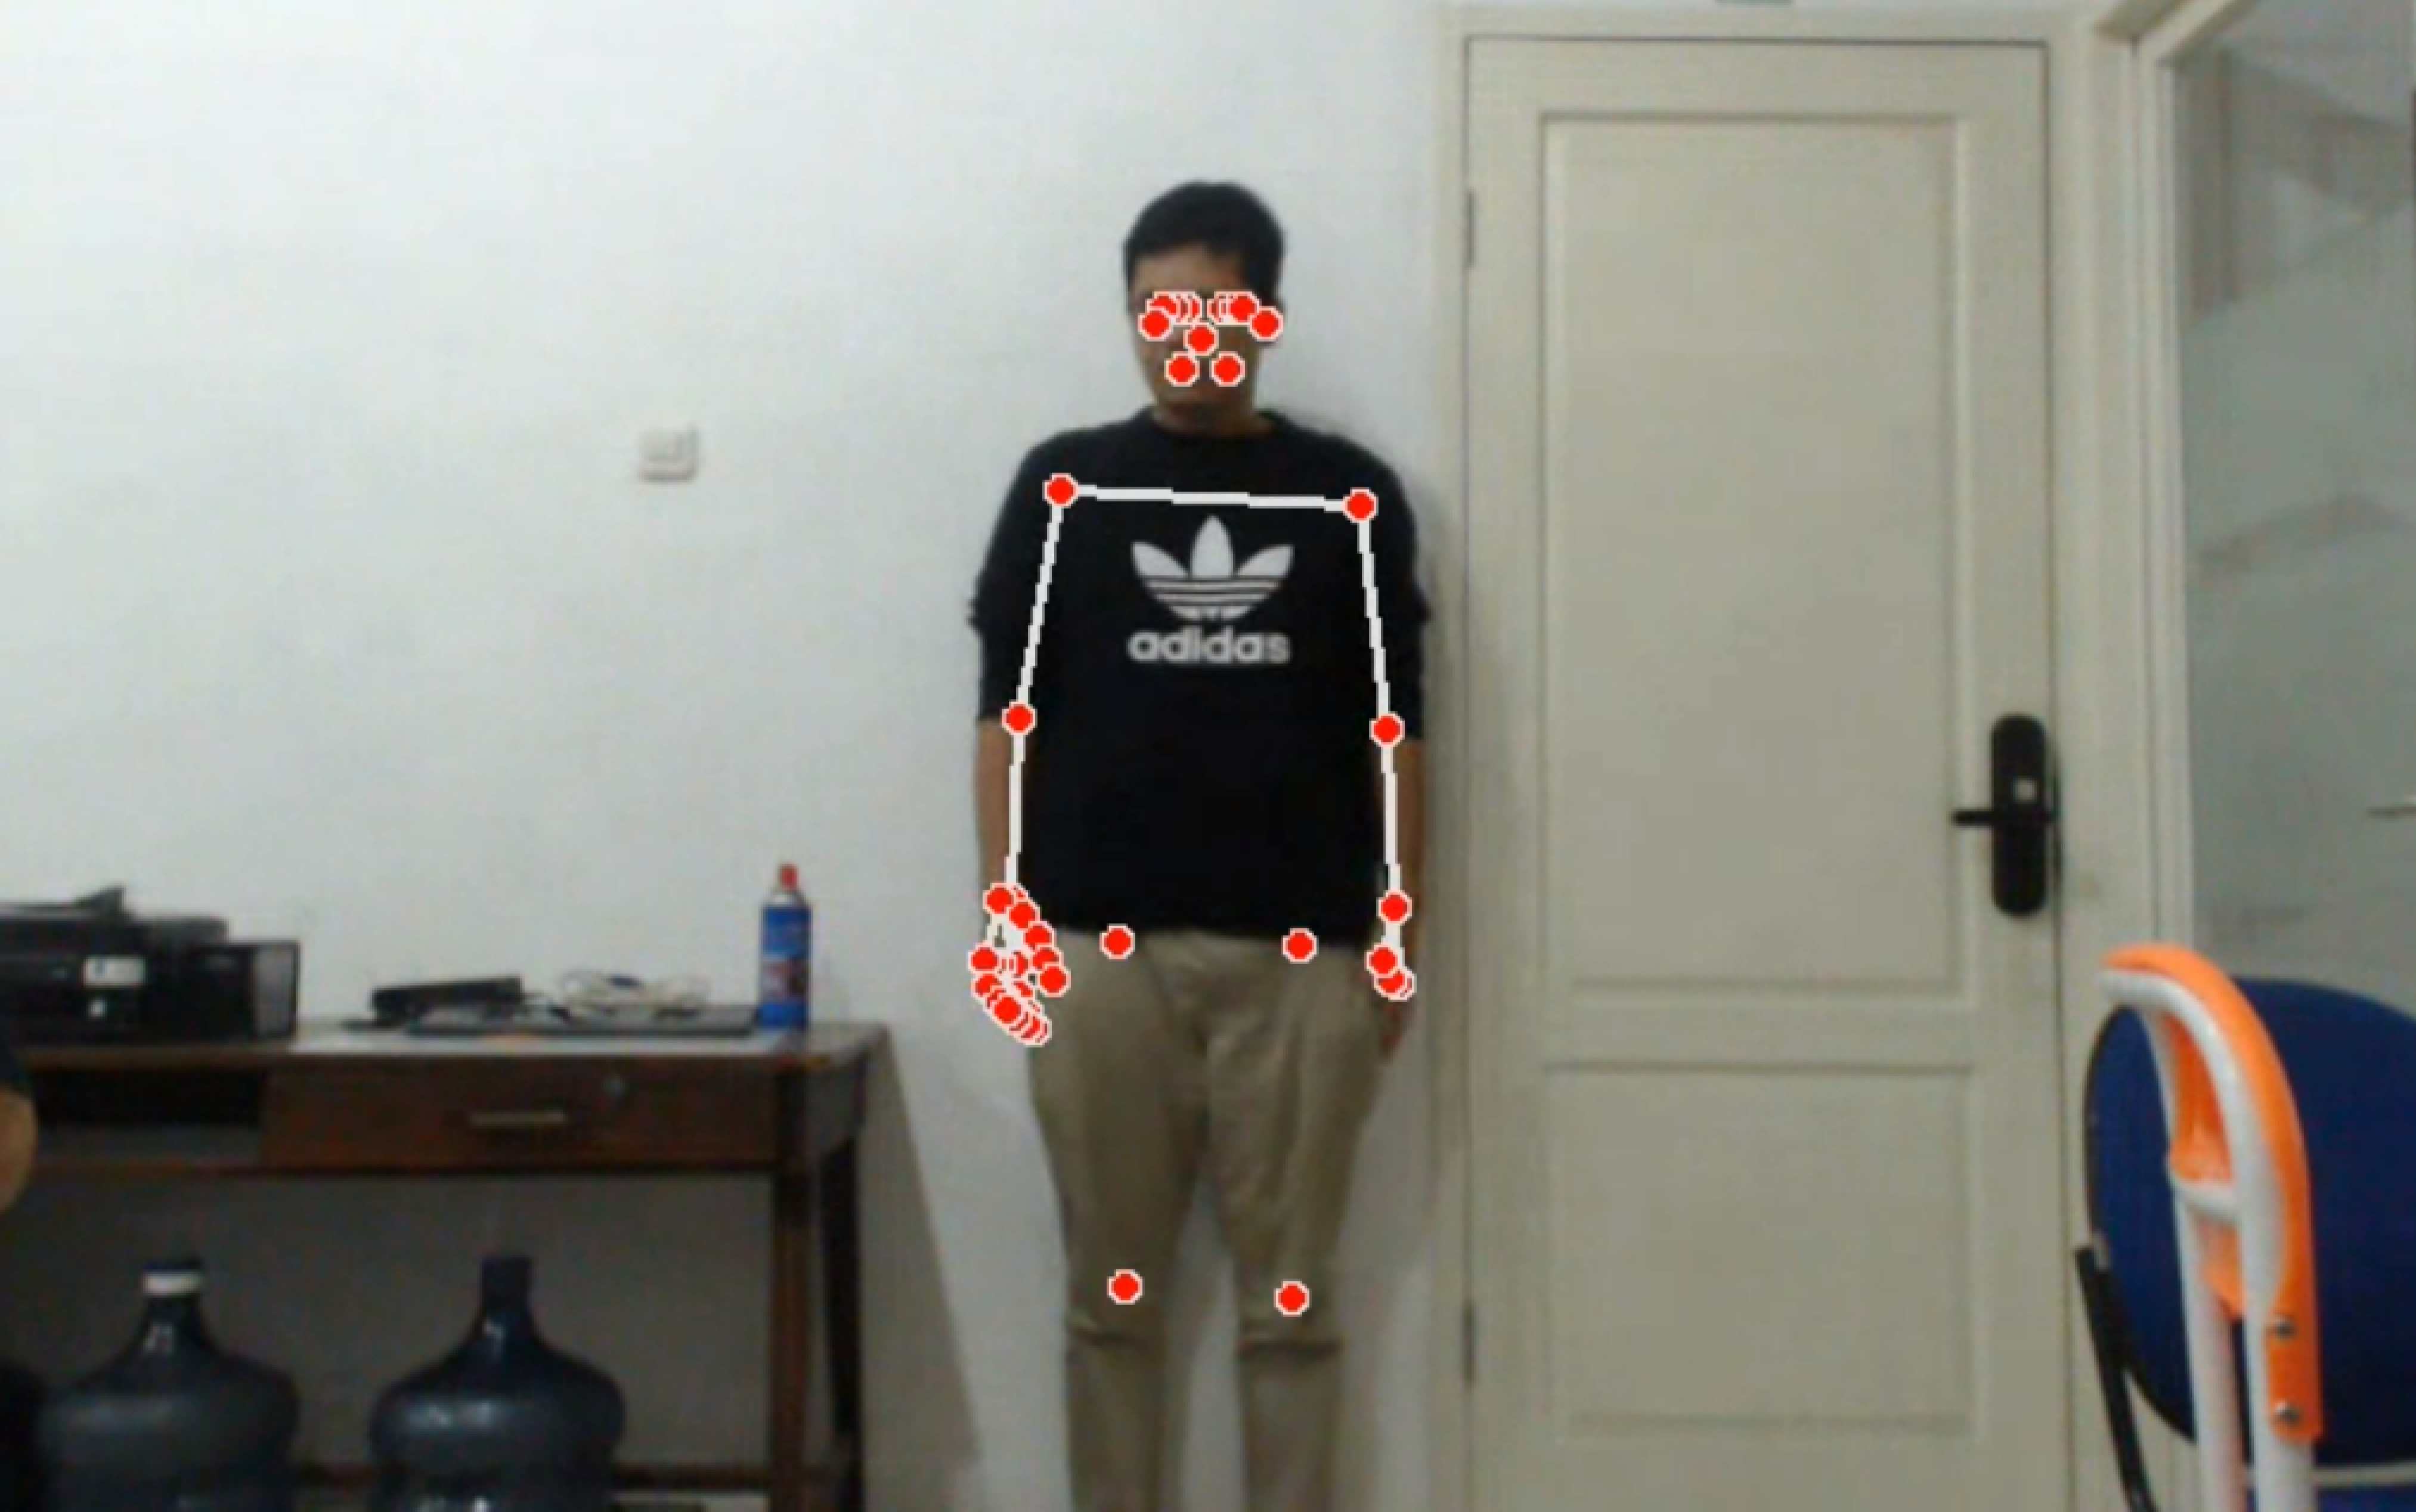
\includegraphics[scale=0.3]{gambar/bab4-evan.png}                 \\
  \hline
\end{longtable}

Pada pengujian dengan menggunakan subjek yang berbeda ini dilakukan untuk memahami bagaimana performa model pada pengguna selain darii penulis. Hal ini dilakukan demi melihat apakah model berhasil beradaptasi terhadap data yang bukan merupakan dataset yang digunakan dalam \emph{training} sehingga kedepannya dapat digunakan oleh kalangan luas. Adapun subjek yang akan diujikan berjumlah 2, yaitu 1 perempuan dan 1 laki - laki. Adapun gambaran subjek yang akan diujikan dapat dilihat pada tabel \ref{tb:kondisisubjek}. 

Model penerjemah bahasa Indonesia (BISINDO) yang akan digunakan pada pengujian ini adalah model pada bagian \ref{sec:analisismodel3} karena merupakan model yang menghasilkan klasifikasi yang terbaik jika dibandingkan dengan model lainnya. Untuk setiap intensitas cahaya akan dilakukan pengujian sebanyak tiga kali dengan jarak terhadap kamera sebesar 300 cm dan intensitas cahaya yang berkisar pada nilai 125 lux atau kondisi ruangan terang. Pada setiap pengujian akan dicari hasil klasifikasi model, waktu yang dibutuhkan model untuk menghasilkan klasifikasi bahasa isyarat berdasarkan data koordinat yang diberikan(\emph{processing time}), dan waktu total yang dibutuhkan dalam menghasilkan klasifikasi bahasa isyarat (\emph{complete time}).  

\subsection{Pengujian Subjek Perempuan}
\label{sec:analisisperempuan}

\begin{longtable}{|c|c|c|c|}
  \caption{Pengujian Pertama Model di Subjek Berbeda Perempuan}
  \label{tb:prediksiperempuan1}                                   \\
  \hline
  \rowcolor[HTML]{C0C0C0}
  \textbf{Kosakata} & \textbf{Klasifikasi Model} & \textbf{\emph{Processing Time}} & \textbf{\emph{Complete Time}}\\
  \hline
  Maaf              & \textcolor{red}{Tolong}       & 0.09316182136535645 detik                           & 3.208651542663574 detik                                \\
  Tolong            & Tolong                        & 0.0934598445892334 detik                            & 2.874863147735596 detik                                \\
  Nama              & Nama                          & 0.09218382835388184 detik                           & 3.2549500465393066 detik                                 \\
  Saya              & Saya                          & 0.09529590606689453 detik                           & 3.128707408905029 detik                                \\
  Siapa              & Siapa                        & 0.09517526626586914 detik                           & 2.9302382469177246 detik                                 \\
  Rumah             & \textcolor{red}{Delete}       & 0.1019589900970459 detik                            & 3.019108772277832 detik                                \\
  Delete            & Delete                        & 0.10392284393310547 detik                           & 3.0571460723876953 detik                                 \\
  Standby           & Standby                       & 0.09529590606689453 detik                           & 1.4797425270080564 detik                                 \\
  Translate         & Translate                     & 0.0931706428527832 detik                            & 2.943220138549805 detik                                \\
  \hline
\end{longtable}

\begin{longtable}{|c|c|c|c|}
  \caption{Pengujian Kedua Model di Subjek Berbeda Perempuan}
  \label{tb:prediksiperempuan2}                                   \\
  \hline
  \rowcolor[HTML]{C0C0C0}
  \textbf{Kosakata} & \textbf{Klasifikasi Model} & \textbf{\emph{Processing Time}} & \textbf{\emph{Complete Time}}\\
  \hline
  Maaf              & Maaf                         & 0.09658217430114746 detik                           & 3.1087589263916016 detik                                  \\
  Tolong            & Tolong                       & 0.0983424186706543 detik                            & 2.8928446769714355 detik                                  \\
  Nama              & Nama                         & 0.09464740753173828 detik                           & 2.980277538299561 detik                                 \\
  Saya              & Saya                         & 0.09416389465332031 detik                           & 2.925252914428711 detik                                 \\
  Siapa             & Siapa                        & 0.0978078842163086 detik                            & 2.927734851837158 detik                                 \\
  Rumah             & Rumah                        & 0.09566903114318848 detik                           & 3.064112663269043 detik                                 \\
  Delete            & Delete                       & 0.10792422294616699 detik                           & 3.3718514442443848 detik                                  \\
  Standby           & Standby                      & 0.09643745422363281 detik                           & 1.5385866165161133 detik                                  \\
  Translate         & Translate                    & 0.10363197326660156 detik                           & 2.9689049720764165 detik                                  \\
  \hline
\end{longtable}

\newpage
\begin{longtable}{|c|c|c|c|}
  \caption{Pengujian Ketiga Model di Subjek Berbeda Perempuan}
  \label{tb:prediksiperempuan3}                                   \\
  \hline
  \rowcolor[HTML]{C0C0C0}
  \textbf{Kosakata} & \textbf{Klasifikasi Model} & \textbf{\emph{Processing Time}} & \textbf{\emph{Complete Time}}\\
  \hline
  Maaf              & Maaf                        & 0.09667658805847168 detik                           & 3.103616237640381 detik                                 \\
  Tolong            & Tolong                      & 0.09738278388977051 detik                           & 3.0499148368835454 detik                                  \\
  Nama              & Nama                        & 0.09640955924987793 detik                           & 2.927877902984619 detik                                 \\
  Saya              & Saya                        & 0.0947885513305664 detik                            & 1.4657378196716309 detik                                  \\
  Siapa             & Siapa                       & 0.09821367263793945 detik                           & 3.0816650390625 detik                               \\
  Rumah             & Rumah                       & 0.09819889068603516 detik                           & 2.870771884918213 detik                                 \\
  Delete            & Delete                      & 0.11416792869567871 detik                           & 3.0212616920471187 detik                                  \\
  Standby           & Standby                     & 0.09473133087158203 detik                           & 1.5490007400512695 detik                                  \\
  Translate         & Translate                   & 0.09832525253295898 detik                           & 3.1276202201843266 detik                                  \\
  \hline
\end{longtable}

Berdasarkan tiga pengujian yang telah dilakukan, didapatkan bahwa hampir keseluruhan klasifikasi model yang sesuai dengan \emph{class} kosakata. Namun, terdapat beberapa kesalahan model dalam melakukan klasifikasi. Dapat dilihat pada tabel \ref{tb:prediksiperempuan1} untuk isyarat kosakata "Maaf" diklasifikasikan sebagai "Tolong". Hal ini dapat disebabkan oleh kesalahan pola gerakan isyarat yang digunakan, dimana kurang ditekankannya keunikan atau \emph{feature} dari masing - masing gerakan bahasa isyarat.  Secara garis besar, hasil pengujian ini menunjukkan bahwa model dengan mudah dapat mengklasifikasikan bahasa isyarat yang diperagakan oleh pengguna dengan jenis kelamin perempuan dengan akurasi sebesar 92.5\%. 

Apabila dilihat berdasarkan waktu pemrosesan, rata - rata waktu yang dibutuhkan model untuk menghasilkan klasifikasi bahasa isyarat (\emph{processing time}) adalah 0.098 detik dan rata - rata waktu yang dibutuhkan dalam menghasilkan klasifikasi bahasa isyarat (\emph{complete time}) adalah 2.810 detik. Hal ini menunjukkan bahwa pada subjek perempuan yang berbeda dengan penulis tidak mempengaruhi nilai \emph{processing time} dan \emph{complete time}. Juga data ini semakin menguatkan bahwa model telah dapat beradaptasi dengan subjek yang berbeda dengan penulis.  

\subsection{Pengujian Subjek Laki - Laki}
\label{sec:analisislaki}

\begin{longtable}{|c|c|c|c|}
  \caption{Pengujian Pertama Model di Subjek Berbeda Laki - Laki}
  \label{tb:prediksilaki1}                                   \\
  \hline
  \rowcolor[HTML]{C0C0C0}
  \textbf{Kosakata} & \textbf{Klasifikasi Model} & \textbf{\emph{Processing Time}} & \textbf{\emph{Complete Time}}\\
  \hline
  Maaf              & \textcolor{red}{Tolong}        & 0.10172176361083984 detik                           & 3.0670595169067383 detik                                  \\
  Tolong            & Tolong                         & 0.09742546081542969 detik                           & 3.017871379852295 detik                                 \\
  Nama              & Nama                           & 0.09616494178771973 detik                           & 3.0398440361022954 detik                                  \\
  Saya              & Saya                           & 0.10310554504394531 detik                           & 1.4680695533752441 detik                                  \\
  Siapa             & Siapa                          & 0.10661101341247559 detik                           & 2.922499179840088 detik                                 \\
  Rumah             & \textcolor{red}{Delete}        & 0.08926630020141602 detik                           & 2.829294204711914 detik                                 \\
  Delete            & Delete                         & 0.09601879119873047 detik                           & 3.159763813018799 detik                                 \\
  Standby           & Standby                        & 0.09913754463195801 detik                           & 1.5385866165161133 detik                                  \\
  Translate         & Translate                      & 0.10099458694458008 detik                           & 2.9112768173217773 detik                                  \\
  \hline
\end{longtable}

\newpage
\begin{longtable}{|c|c|c|c|}
  \caption{Pengujian Kedua Model di Subjek Berbeda Laki - Laki}
  \label{tb:prediksilaki2}                                   \\
  \hline
  \rowcolor[HTML]{C0C0C0}
  \textbf{Kosakata} & \textbf{Klasifikasi Model} & \textbf{\emph{Processing Time}} & \textbf{\emph{Complete Time}}\\
  \hline
  Maaf              & Maaf                         & 0.10624909400939941 detik                           & 2.9753994941711426 detik                                  \\
  Tolong            & Tolong                       & 0.09604954719543457 detik                           & 2.9878664016723637 detik                                  \\
  Nama              & Nama                         & 0.09938287734985352 detik                           & 2.855043411254883 detik                                 \\
  Saya              & Saya                         & 0.09951472282409668 detik                           & 1.5473628044128418 detik                                  \\
  Siapa             & Siapa                        & 0.08862924575805664 detik                           & 2.881293296813965 detik                                 \\
  Rumah             & Rumah                        & 0.08926630020141602 detik                           & 2.879476547241211 detik                                 \\
  Delete            & Delete                       & 0.09708309173583984 detik                           & 3.097364902496338 detik                                 \\
  Standby           & Standby                      & 0.10267424583435059 detik                           & 1.5490007400512695 detik                                  \\
  Translate         & Translate                    & 0.10302090644836426 detik                           & 3.1186795234680176 detik                                  \\
  \hline
\end{longtable}

\begin{longtable}{|c|c|c|c|}
  \caption{Pengujian Ketiga Model di Subjek Berbeda Laki - Laki}
  \label{tb:prediksilaki3}                                   \\
  \hline
  \rowcolor[HTML]{C0C0C0}
  \textbf{Kosakata} & \textbf{Klasifikasi Model} & \textbf{\emph{Processing Time}} & \textbf{\emph{Complete Time}}\\
  \hline
  Maaf              & Maaf                          & 0.09524083137512207 detik                           & 3.0119776725769043 detik                                  \\
  Tolong            & Tolong                        & 0.10116004943847656 detik                           & 3.0259251594543457 detik                                 \\
  Nama              & Nama                          & 0.10364699363708496 detik                           & 2.9966139793395996 detik                                 \\
  Saya              & Saya                          & 0.0972299575805664 detik                            & 1.4724183082580566 detik                                 \\
  Siapa             & Siapa                         & 0.09995222091674805 detik                           & 2.967231273651123 detik                                \\
  Rumah             & Rumah                         & 0.08926630020143602 detik                           & 2.9637622833251953 detik                                 \\
  Delete            & Delete                        & 0.09006118774414062 detik                           & 2.9045462608337402 detik                                 \\
  Standby           & Standby                       & 0.10000467300415039 detik                           & 2.028508186340332 detik                                \\
  Translate         & Translate                     & 0.10082817077636719 detik                           & 3.1959056854248047 detik                                 \\
  \hline
\end{longtable}

Berdasarkan tiga pengujian yang telah dilakukan, didapatkan bahwa hampir keseluruhan klasifikasi model yang sesuai dengan \emph{class} kosakata. Namun, terdapat beberapa kesalahan model dalam melakukan klasifikasi. Dapat dilihat pada tabel \ref{tb:prediksilaki1} untuk kosakata isyarat "Maaf" diklasifikasikan sebagai "Tolong". Hal ini dapat disebabkan oleh kesalahan pola gerakan isyarat yang digunakan, dimana kurang ditekankannya keunikan atau \emph{feature} dari masing - masing gerakan bahasa isyarat.  Secara garis besar, hasil pengujian ini menunjukkan bahwa model dengan mudah dapat mengklasifikasikan bahasa isyarat yang diperagakan oleh pengguna dengan jenis kelamin perempuan dengan akurasi sebesar 92.5\%. 

Apabila dilihat berdasarkan waktu pemrosesan, rata - rata waktu yang dibutuhkan model untuk menghasilkan klasifikasi bahasa isyarat (\emph{processing time}) adalah 0.098 detik dan rata - rata waktu yang dibutuhkan dalam menghasilkan klasifikasi bahasa isyarat (\emph{complete time}) adalah 2.682 detik. Hal ini menunjukkan bahwa pada subjek yang berbeda dengan penulis tidak mempengaruhi \emph{processing time} dan \emph{complete time}. Data ini juga menunjukkan bahwa proses normalisasi yang dilakukan telah berhasil dan memudahkan model untuk mengklasifikasikan gerakan bahasa isyarat secara \emph{general} atau menyeluruh.  

\newpage
\subsection{Rangkuman Pengujian Subjek Berbeda}
\label{sec:analisissubjekberbeda}

\begin{longtable}{|c|c|c|c|}
  \caption{Rangkuman Pengujian Subjek Berbeda}
  \label{tb:evaluasiSubjek}                                   \\
  \hline
  \rowcolor[HTML]{C0C0C0}
  \textbf{Subjek} & \textbf{Akurasi} & \emph{\textbf{Avg. Processing Time}} & \emph{\textbf{Avg. Complete Time}} \\
  \hline
  Perempuan & 0.93   & 0.0988 detik & 2.6636 detik \\
  Laki - Laki & 0.93 & 0.0973 detik & 2.8191 detik \\
  \hline
\end{longtable}

Secara keseluruhan, dapat dilihat bahwa model dapat bekerja untuk melakukan klasifikasi berdasarkan gerakan isyarat dari subjek yang berbeda dengan penulis. Normalisasi data yang dilakukan telah berhasil menggeneralisasi data sehingga model dapat menghasilkan klasifikasi yang baik meskipun berasal dari subjek yang berbeda dari penulis. Hal ini dibuktikan dengan akurasi pada subjek laki - laki dan perempuan bernilai 0.93 atau 93\%. Adapun nilai dari \emph{average processing time} dan \emph{average complete time} berkisar pada 0.09 detik dan 2.6 detik. Data ini tidak jauh berbeda dengan bebrapa pengujian sebelumnya yang telah dilakukan oleh penulis.

\section{Pengujian Pembentukan Kalimat dan Konversi Suara}
\label{sec:analisiskalimat}

Pada pengujian pembentukan kalimat dan konversi suara ini dilakukan untuk memahami bagaimana sistem penerjemah bahasa isyarat Indonesia (BISINDO) jika digunakan untuk membentuk kalimat dan melakukan konversi suara berdasarkan kalimat yang dibentuk. Adapun sistematika dalam pembentukan kalimat dan konversi ini mengacu dengan \emph{flowchart} yang telah dijelaskan pada sub bab \ref{sec:metodologisistemkontrol}. Kombinasi kata untuk membentuk kalimat pada sistem ini dapat dilihat pada tabel \ref{tb:kalimatpengujian}. Perlu diperhatikan bahwa untuk mendeteksi kosakata dan mengontrol sistem (\emph{translate} dan \emph{delete}) memerlukan pengguna untuk berada di keadaan \emph{standby} terlebih dahulu. Pembentukan kalimat dan konveri suara pada pengujian ini dilakukan secara sekuensial dengan memastikan bahwa setiap kosakata benar terklasifikasi. Kemudian, kalimat akan diterjemahkan dengan melakukan gerakan isyarat kontrol "\emph{translate}" dan diakhiri dengan melakukan gerakan isyarat kontrol "\emph{delete}" untuk memastikan bahwa kosakata terakhir berhasil dihapus. Pengulangan bahasa isyarat dilakukan maksimal sebanyak tiga kali.

\begin{longtable}{|c|c|}
  \caption{Kalimat Pengujian}
  \label{tb:kalimatpengujian}                                   \\
  \hline
  \rowcolor[HTML]{C0C0C0}
  \textbf{Kombinasi Kosakata} & \textbf{Kalimat Akhir}  \\
  \hline
  "Maaf" + "Siapa" + "Nama"            &  "Maaf siapa nama kamu?"               \\

  "Maaf" + "Tolong "+ "Saya"            & "Maaf tolong bantu saya"                 \\
  
  "Maaf" + "Rumah" + "Siapa"            & "Maaf ini rumah siapa?"                 \\

  "Rumah" + "Saya"            & "Ini rumah saya"                 \\

  "Rumah" + "Siapa"            & "Ini rumah siapa"                 \\

  "Siapa" + "Nama"            & "Siapa nama kamu?"                 \\

  "Tolong" + "Saya"            & "Tolong bantu saya"                 \\
  \hline
\end{longtable}

Model penerjemah bahasa Indonesia (BISINDO) yang akan digunakan pada pengujian ini adalah model pada bagian \ref{sec:analisismodel3} karena merupakan model yang menghasilkan klasifikasi yang terbaik jika dibandingkan dengan model lainnya. Untuk setiap kombinasi kalimat akan dilakukan pengujian sebanyak satu kali dengan kondisi ruangan yang memiliki intensitas cahaya yang terang (berkisar pada 125 lux) dan jarak kamera dengan pengguna bernilai 300 cm. Pada setiap kombinasi kalimat akan dicari hasil klasifikasi model, waktu yang dibutuhkan model untuk menghasilkan klasifikasi bahasa isyarat berdasarkan data koordinat yang diberikan(\emph{processing time}), dan waktu total yang dibutuhkan dalam menghasilkan klasifikasi bahasa isyarat (\emph{complete time}).  

\begin{longtable}{|c|c|c|c|}
  \caption{Pengujian Pembentukan Kalimat Pertama}
  \label{tb:prediksikombinasi1}                                   \\
  \hline
  \rowcolor[HTML]{C0C0C0}
  \textbf{Kosakata} & \textbf{Klasifikasi Model} & \textbf{\emph{Processing Time}} & \textbf{\emph{Complete Time}}\\
  \hline
  Maaf                & Maaf                          & 0.09733414649963379 detik                           & 3.103902339935303 detik                                 \\
  Siapa               & Siapa                         & 0.0981595516204834 detik                            & 2.81724214553833 detik                                \\
  Nama                & Nama                          & 0.09517359733581543 detik                           & 3.097071647644043 detik                                 \\
  Delete              & Delete                        & 0.09404182434082031 detik                           & 3.1426548957824707 detik                                  \\
  Translate           & Translate                     & 0.09448504447937012 detik                           & 2.94607400894165 detik                                \\
  \hline
\end{longtable}

\begin{longtable}{|c|c|c|c|}
  \caption{Pengujian Pembentukan Kalimat Kedua}
  \label{tb:prediksikombinasi2}                                   \\
  \hline
  \rowcolor[HTML]{C0C0C0}
  \textbf{Kosakata} & \textbf{Klasifikasi Model} & \textbf{\emph{Processing Time}} & \textbf{\emph{Complete Time}}\\
  \hline
  Maaf              & Maaf                          & 0.10064482688903809 detik                           & 2.822299003601074 detik                                 \\
  Tolong            & Tolong                        & 0.09766435623168945 detik                           & 2.844550609588623 detik                                 \\
  Saya              & Nama                          & 0.09680485725402832 detik                           & 2.9134011268615723 detik                                  \\
  Delete              & Delete                      & 0.09553837776184082 detik                           & 3.1421828269958496 detik                                  \\
  Translate              & Translate                & 0.09472537040710449 detik                           & 2.8847408294677734 detik                                  \\
  \hline
\end{longtable}

\begin{longtable}{|c|c|c|c|}
  \caption{Pengujian Pembentukan Kalimat Ketiga}
  \label{tb:prediksikombinasi3}                                   \\
  \hline
  \rowcolor[HTML]{C0C0C0}
  \textbf{Kosakata} & \textbf{Klasifikasi Model} & \textbf{\emph{Processing Time}} & \textbf{\emph{Complete Time}}\\
  \hline
  Maaf              & Maaf                          & 0.10550785064697266 detik                           & 2.969491481781006 detik                                 \\
  Rumah            & Tolong                         & 0.0971059799194336  detik                           & 2.9895544052124023 detik                                  \\
  Siapa              & Nama                         & 0.10715579986572266 detik                           & 2.9179072380065922 detik                                  \\
  Delete              & Delete                      & 0.0979464054107666  detik                           & 2.9804134368896484 detik                                  \\
  Translate              & Translate                & 0.10163474082946777 detik                           & 2.958190441131592 detik                                 \\
  \hline
\end{longtable}

\begin{longtable}{|c|c|c|c|}
  \caption{Pengujian Pembentukan Kalimat Keempat}
  \label{tb:prediksikombinasi4}                                   \\
  \hline
  \rowcolor[HTML]{C0C0C0}
  \textbf{Kosakata} & \textbf{Klasifikasi Model} & \textbf{\emph{Processing Time}} & \textbf{\emph{Complete Time}}\\
  \hline
  Rumah               & \textcolor{red}{Delete}       & 0.09740185737609863 detik                           & 3.042304515838623 detik                                 \\
  Saya                & Saya                          & 0.0987851619720459 detik                            & 1.4961934089660645 detik                                  \\
  Delete              & Delete                        & 0.09497356414794922 detik                           & 2.9061841964721684 detik                                  \\
  Translate           & Translate                     & 0.10316205024719238 detik                           & 2.943763732910156 detik                                 \\
  \hline
\end{longtable}

\newpage
\begin{longtable}{|c|c|c|c|}
  \caption{Pengujian Pembentukan Kalimat Kelima}
  \label{tb:prediksikombinasi5}                                   \\
  \hline
  \rowcolor[HTML]{C0C0C0}
  \textbf{Kosakata} & \textbf{Klasifikasi Model} & \textbf{\emph{Processing Time}} & \textbf{\emph{Processing Time}}\\
  \hline
  Rumah               & Rumah                         & 0.09344840049743652 detik                           & 1.5613818168640137 detik                                  \\
  Siapa               & Siapa                         & 0.09488558769226074 detik                           & 1.4586281776428223 detik                                  \\
  Delete              & Delete                        & 0.09873461723327637 detik                           & 3.033885955810547  detik                                 \\
  Translate           & Translate                     & 0.1056978702545166 detik                            & 2.9063844680786133 detik                                  \\
  \hline
\end{longtable}

\begin{longtable}{|c|c|c|c|}
  \caption{Pengujian Pembentukan Kalimat Keenam}
  \label{tb:prediksikombinasi6}                                   \\
  \hline
  \rowcolor[HTML]{C0C0C0}
  \textbf{Kosakata} & \textbf{Klasifikasi Model} & \textbf{\emph{Processing Time}} & \textbf{\emph{Complete Time}}\\
  \hline
  Siapa               & Siapa                         & 0.10315442085266113 detik                           & 3.042304515838623 detik                                 \\
  Nama                & Nama                          & 0.0998544692993164  detik                           & 1.4961934089660645 detik                                  \\
  Delete              & Delete                        & 0.09890484809875488 detik                           & 2.9061841964721684 detik                                  \\
  Translate           & Translate                     & 0.10316205024719238 detik                           & 2.943763732910156 detik                                 \\
  \hline
\end{longtable}

\begin{longtable}{|c|c|c|c|}
  \caption{Pengujian Pembentukan Kalimat Ketujuh}
  \label{tb:prediksikombinasi7}                                   \\
  \hline
  \rowcolor[HTML]{C0C0C0}
  \textbf{Kosakata} & \textbf{Klasifikasi Model} & \textbf{\emph{Processing Time}} & \textbf{\emph{Complete Time}}\\
  \hline
  Tolong              & Tolong                        & 0.10103940963745117 detik                          & 3.0083799362182617 detik                                  \\
  Saya                & Saya                          & 0.10042452812194824 detik                          & 2.944457530975342 detik                                 \\
  Delete              & Delete                        & 0.0952444076538086 detik                           & 3.03605318069458  detik                                \\
  Translate           & Translate                     & 0.10302400588989258 detik                          & 3.0155038833618164 detik                                  \\
  \hline
\end{longtable}

% \begin{longtable}{|c|c|}
%   \caption{Waktu \emph{Translate} Kombinasi Kalimat}
%   \label{tb:waktutranslate}                                   \\
%   \hline
%   \rowcolor[HTML]{C0C0C0}
%   \textbf{Kalimat} & \textbf{Waktu Penyuaraan Kalimat}\\
%   \hline
%   Maaf siapa nama kamu?              & 1.9165489673614502                               \\
%   Maaf tolong bantu saya            & 1.824713945388794                            \\
%   Maaf ini rumah siapa?              & 1.9595482349395752                         \\
%   Ini rumah saya              & 1.5204029083251953                             \\
%   Ini rumah siapa?              & 1.605020523071289                             \\
%   Siapa nama kamu?              & 1.606485366821289                             \\
%   Tolong bantu saya              & 1.5231249332427979                             \\
%   \hline
% \end{longtable}

Untuk kalimat yang terdiri dari kombinasi tiga kosakata, yaitu kalimat pertama, kalimat kedua, dan kalimat ketiga telah berhasil dibentuk. Hal ini dapat dilihat dari untuk kombinasi kosakata pembentuk kalimat tersebut telah berhasil diklasifikasikan dengan akurasi sebesar 100\% (dapat dilihat pada tabel \ref{tb:prediksikombinasi1}, tabel \ref{tb:prediksikombinasi2}, dan tabel \ref{tb:prediksikombinasi3}). Pada kalimat pertama, rata - rata \emph{processing time} bernilai 0.096 detik dan \emph{complete time} bernilai 3.021 detik. Pada kalimat kedua, rata - rata \emph{processing time} bernilai 0.097 detik dan \emph{complete time} bernilai 2.921 detik. Pada kalimat ketiga, rata - rata \emph{processing time} bernilai 0.102 detik dan \emph{complete time} bernilai 2.963 detik. Dapat dilihat bahwa meskipun gerakan bahasa isyarat dilakukan secara sekuensial, tetap dapat menghasilkan klasifikasi akurasi yang baik.

Untuk kalimat yang terdiri dari kombinasi dua kosakata, yaitu kalimat kelima, keenam, dan ketujuh telah berhasil dibentuk. Hal ini dapat dilihat dari kombinasi kosakata pembentuk kalimat tersebut telah berhasil diklasifikasikan dengan akurasi sebesar 93.75\% (dapat dilihat pada tabel \ref{tb:prediksikombinasi5}, \ref{tb:prediksikombinasi6}, \ref{tb:prediksikombinasi7}). Pada kalimat kelima, rata - rata \emph{processing time} bernilai 0.098 detik dan \emph{complete time} bernilai 2.240 detik. Pada kalimat keenam, rata - rata \emph{processing time} bernilai 0.100 detik dan \emph{complete time} bernilai 2.199 detik.Pada kalimat ketujuh, rata - rata \emph{processing time} bernilai 0.100 detik dan \emph{complete time} bernilai 3.001 detik. Dapat dilihat bahwa untuk \emph{complete time} relatif lebih cepat pada kalimat dengan kombinasi tiga kosakata jika dibandingkan dengan kalimat dengan kombinasi dua kosakata.

Namun, pada kalimat keempat ("Ini rumah saya") terdapat kosakata yang salah sehingga menyebabkan gagalnya terbentuk kalimat tersebut dalam pengujian yang dilakukan secara sekue\\nsial. Isyarat kosakata "Rumah" diklasifikasikan sebagai "Delete". Hal ini dapat disebabkan oleh adanya kemiripan gerakan antara kedua kosakata tersebut. rata - rata \emph{processing time} bernilai 0.099 detik dan \emph{complete time} bernilai 2.597 detik.

\subsection{Rangkuman Pengujian Pembentukan Kalimat dan Konveri Suara}
\label{sec:analisikalimatsuara}

\begin{longtable}{|c|c|c|c|}
  \caption{Rangkuman Pengujian Pembentukan Kalimat dan Konveri Suara}
  \label{tb:evaluasiKalimatdanSuara}                                   \\
  \hline
  \rowcolor[HTML]{C0C0C0}
  \textbf{Kosakata} & \textbf{Akurasi} & \emph{\textbf{Avg. Processing Time}} & \emph{\textbf{Avg. Complete Time}} \\
  \hline
  2 kosakata & 1.00 & 0.0993 detik & 2.8303 detik \\
  3 kosakata & 0.93 & 0.0981 detik & 2.0513 detik \\
  \hline
\end{longtable}

Secara keseluruhan, dapat dilihat bahwa sistem penerjemah dapat melakukan klasifikasi dengan baik dalam menerjemahkan gerakan isyarat yang dilakukan secara sekuensial. Hal ini tidak berdampak secara signifikan terhadap \emph{average processing time} dan \emph{average complete time}. Akurasi klasifikasi masih sangat baik, dimana pada kalimat dengan 2 kosakata bernilai 1.00 atau 100\% dan 3 kosakata bernilai 0.93 atau 93\%. Pada kalimat dengan 3 kosakata, hanya 1 kalimat yang tidak berhasil untuk dibentuk, yaitu kalimat "Ini rumah saya" sehingga tingkat keberhasilan sistem penerjemah dalam membentuk kalimat adalah sebesar 85.7\%.

% Untuk kalimat yang terdiri dari kombinasi tiga kosakata, pada kombinasi kalimat pertama didapat bahwa keseluruhan kosakata bahasa isyarat untuk kalimat "Maaf siapa nama kamu?" telah berhasil dibentuk. Hal ini dapat dilihat untuk seluruh kombinasi kosakata yang telah berhasil diklasifikasikan dengan akurasi sebesar 100\%. Untuk rata - rata \emph{processing time} dan \emph{complete time} adalah 0.096 detik  dan 3.021 detik. Pada kombinasi kalimat kedua, keseluruhan kosakata bahasa isyarat untuk kalimat "Maaf tolong bantu saya?" telah berhasil dibentuk. Hal ini dapat dilihat untuk seluruh kombinasi kosakata yang telah berhasil diklasifikasikan dengan akurasi sebesar 100\%. Untuk rata - rata \emph{processing time} dan \emph{complete time} adalah 0.097 detik  dan 2.921 detik. Pada kombinasi kalimat ketiga, keseluruhan kosakata bahasa isyarat untuk kalimat "Maaf ini rumah siapa?" telah berhasil dibentuk. Hal ini dapat dilihat untuk seluruh kombinasi kosakata yang telah berhasil diklasifikasikan dengan akurasi sebesar 100\%. Untuk rata - rata \emph{processing time} dan \emph{complete time} adalah 0.102 detik  dan 2.963 detik.

% Untuk kalimat yang terdiri dari kombinasi dua kosakata, pada kombinasi kalimat keempat didapat bahwa keseluruhan kosakata bahasa isyarat untuk kalimat "Ini rumah saya" tidak berhasil dibentuk. Hal ini disebabkan oleh kosakata "Rumah" diklasifikasikan sebagai "Delete". Untuk rata - rata \emph{processing time} dan \emph{complete time} adalah 0.096 detik dan 3.021 detik. Pada kombinasi kalimat keenam, keseluruhan bahasa isyarat untuk kalimat "Maaf tolong bantu saya"  telah berhasil dibentuk. Hal ini dapat dilihat untuk seluruh kombinasi kosakata telah berhasil diklasifikasikan dengan akurasi sebesar 100\%.  Untuk rata - rata \emph{processing time} dan \emph{complete time} adalah 0.098 detik  dan 2.240 detik.

% \section{Pengujian Performa NUC}
% \label{sec:analisisnuc}
% \section{Evaluasi Pengujian}
% \label{sec:analisispengujian}

% Dari pengujian yang \lipsum[1]

% % Contoh pembuatan tabel


% \lipsum[2-4]

\cleardoublepage

% Bab 5 penutup
\chapter{PENUTUP}
\label{chap:penutup}

% Ubah bagian-bagian berikut dengan isi dari penutup
Pada bab ini akan dipaparkan kesimpulan dari hasil pengujian yang telah dilakukan. Kesimpulan ini akan menjawab permasalahan yang diangkat dengan merujuk pada tujuan dari pelaksanaan tugas akhir ini. Pada bab ini juga dipaparkan saran mengenai hal yang dapat dilakukan untuk mengembangkan penelitian dengan topik yang sama.

\section{Kesimpulan}
\label{sec:kesimpulan}

Berdasarkan hasil pengujian yang telah dilakukan dalam tugas akhir ini, dapat diambil kesimpulan sebagai berikut:

\begin{enumerate}[nolistsep]

  \item Model LSTM memiliki performa paling baik dengan penggunaan \emph{layer TimeDistributed} yang diikuti dengan 2 \emph{layer} LSTM pada akurasi 99\%.
  \item Sistem penerjemah bahasa isyarat telah berhasil diimplementasikan pada Intel \emph{Next Unit Computing} (NUC) dan dapat berjalan secara \emph{real time}. 
  \item Intensitas cahaya 125 lux atau kondisi ruangan terang menghasilkan klasifikasi terbaik dengan akurasi sebesar 100\%.
  \item Jarak kamera terhadap pengguna sebesar 300 cm menghasilkan klasifikasi terbaik dengan akurasi sebesar sebesar 100\%.
  \item Model berhasil beradaptasi dengan subjek selain penulis dengan akurasi sebesar 92.5\% untuk subjek perempeuan dan laki - laki.
  \item Sistem penerjemah dapat membentuk kalimat dan mengkonversi menjadi suara dengan tingkat keberhasilan sebesar 85.7\%.


\end{enumerate}

\section{Saran}
\label{chap:saran}

Berdasarkan hasil yang diperoleh dari tugas akhir ini, saran yang dapat dipertimbangkan untuk pengembangan lebih lanjut adalah sebagai berikut:

\begin{enumerate}[nolistsep]

  \item Menambahkan variasi jarak, intensitas cahaya, dan subjek berbeda untuk menguji bagaim\\ana kemampuan model dalam beradaptasi dengan serangkaian perubahan yang terjadi.
  \item Mempertimbangkan menggunakan metode lain, seperti CNN-LSTM untuk dapat melakukan ekstraksi \emph{feature} dalam bentuk citra sehingga dapat melakukan klasifikasi gerakan bahasa isyarat dengan lebih baik dan akurat lagi.

\end{enumerate}

\cleardoublepage

\chapter*{DAFTAR PUSTAKA}
\addcontentsline{toc}{chapter}{DAFTAR PUSTAKA}
\renewcommand\refname{}
\vspace{2ex}
\renewcommand{\bibname}{}
\begingroup
\def\chapter*#1{}
\printbibliography
\endgroup
\cleardoublepage

% Biografi penulis
\begin{center}
  \Large
  \textbf{BIOGRAFI PENULIS}
\end{center}

\addcontentsline{toc}{chapter}{BIOGRAFI PENULIS}

\vspace{2ex}

\begin{wrapfigure}{L}{0.3\textwidth}
  \centering
  \vspace{-3ex}
  % Ubah file gambar berikut dengan file foto dari mahasiswa
  
\includegraphics[width=0.3\textwidth]{gambar/elon.jpg}
  \vspace{-4ex}
\end{wrapfigure}

% Ubah kalimat berikut dengan biografi dari mahasiswa
\name{}, lahir pada \lipsum[1]

\lipsum[2]

\cleardoublepage

\end{document}
